\documentclass[12pt,draftcls]{ucdavisthesisakp}

% PLEASE READ THE MANUAL - ucdavisthesis.pdf (in the package installation directory)

%%%%%%%%%%%%%%%%%%%%%%%%%%%%%%%%%%%%%%%%%%%%%%%%%%%%%%%%%%%%%%%%%%%%%%%%
%                                                                      %
%               LATEX COMMANDS FOR DOCUMENT SETUP                      %
%                                                                      %
%%%%%%%%%%%%%%%%%%%%%%%%%%%%%%%%%%%%%%%%%%%%%%%%%%%%%%%%%%%%%%%%%%%%%%%%

%\usepackage{bookmark}
\usepackage[us,nodayofweek,12hr]{datetime}
\usepackage{graphicx}
\usepackage{subcaption}
\usepackage{tabu}
\usepackage{booktabs}

%\usepackage[square,comma,numbers,sort&compress]{natbib}
%\usepackage{hypernat}
% Other useful packages to try
%\usepackage{amsmath}
%\usepackage{amssymb}
%
% Different fonts to try (uncomment only fontenc and one font at a time)
% (you may need to install these first)
%\usepackage[T1]{fontenc} %enable fontenc package if using one of the fonts below
%\usepackage[adobe-utopia]{mathdesign}
%\usepackage{tgschola}
%\usepackage{tgbonum}
%\usepackage{tgpagella}
%\usepackage{tgtermes}
%\usepackage{fourier}
%\usepackage{fouriernc}
%\usepackage{kmath,kerkis}
%\usepackage{kpfonts}
%\usepackage[urw-garamond]{mathdesign}
%\usepackage[bitstream-charter]{mathdesign}
%\usepackage[sc]{mathpazo}
%\usepackage{mathptmx}
%\usepackage[varg]{txfonts}

\hyphenation{dis-ser-ta-tion blue-print man-u-script pre-par-ing} %add hyphenation rules for words TeX doesn't know


%\renewcommand{\rightmark}{\scriptsize A University of California Davis\ldots \hfill Rev.~\#1.0 \quad Compiled: \currenttime, \today}
% a fancier running header that can be used with draftcls options

%%%%%%%%%%%%%%%%%%%%%%%%%%%%%%%%%%%%%%%%%%%%%%%%%%%%%%%%%%%%%%%%%%%%%%%%
%                                                                      %
%        DOCUMENT SETUP AND INFORMATION FOR PRELIMINARY PAGES          %
%                                                                      %
%%%%%%%%%%%%%%%%%%%%%%%%%%%%%%%%%%%%%%%%%%%%%%%%%%%%%%%%%%%%%%%%%%%%%%%%

\title          {Visualization Techniques to Inform Science-Based Decision-Making
}
%Exact title of your thesis. Indicate italics where necessary by underlining or using italics. Please capitalize the first letter of each word that would normally be capitalized in a title.

\author         {Annie Kathleen Preston}
%Your full name as it appears on University records. Do not use initials.

\dissertationproposal{Doctor of Philosophy}

\authordegrees  {B.S. (Haverford College) 2012}
%Indicate your previous degrees conferred.

\officialmajor  {Computer Science}
%This is your official major as it appears on your University records.

\graduateprogram{Computer Science}
%This is your official graduate program name. Used for UMI abstract.

\degreeyear     {2019}
% Indicate the year in which your degree will be officially conferred.

\degreemonth    {June}
% Indicate the month in which your degree will be officially conferred. Used for UMI abstract.

\committee{Dr. Bernd Hamann}{Dr. Nina Amenta}{Dr. Gunther Weber}{Dr. Zhou Yu}{Dr. Kwan-Liu Ma}
% These are your committee members. The command accepts up to five committee members so be sure to have five sets of braces, even if there are empties.

%%%%%%%%%%%%%%%%%%%%%%%%%%%%%%%%%%%%%%%%%%%%%%%%%%%%%%%%%%%%%%%%%%%%%%%%

%\copyrightyear{2020}
%\nocopyright

%%%%%%%%%%%%%%%%%%%%%%%%%%%%%%%%%%%%%%%%%%%%%%%%%%%%%%%%%%%%%%%%%%%%%%%%

\dedication{\textsl{To someone very important \ldots \\
            a nice dedication.}}

%%%%%%%%%%%%%%%%%%%%%%%%%%%%%%%%%%%%%%%%%%%%%%%%%%%%%%%%%%%%%%%%%%%%%%%%

\abstract{Here, add a condensed version of my proposal outline, in a long-abstract format.}

%%%%%%%%%%%%%%%%%%%%%%%%%%%%%%%%%%%%%%%%%%%%%%%%%%%%%%%%%%%%%%%%%%%%%%%%

\acknowledgments{Acknowledgements to those who helped you get to this point. They should be listed by chapter when appropriate.}

%%%%%%%%%%%%%%%%%%%%%%%%%%%%%%%%%%%%%%%%%%%%%%%%%%%%%%%%%%%%%%%%%%%%%%%%

% Each chapter can be in its own file for easier editing and brought in with the \include command.
% Then use the \includeonly command to speed compilation when working on a particular chapter.
%%% \includeonly{ucdavisthesis_example_Chap1}

\begin{document}

\newcommand{\bibfont}{\singlespacing}
% need this command to keep single spacing in the bibliography when using natbib

\bibliographystyle{IEEEtran}
%many other bibliography styles are available (IEEEtran, mla, etc.). Use one appropriate for your field.

\makeintropages %Processes/produces the preliminary pages

\chapter{Introduction}

\section{Motivation}
\subsection{Machine Learning in Scientific Analysis}
\subsection{Uncertainty, Confidence, and Transparency}

\section{Outline of Contributions}
\chapter{A Visualization Framework for Dark Matter Simulation Data}

\section{Introduction}

Dark matter, the unidentified substance that comprises the vast majority of matter in the universe, generates a wealth of unanswered questions for scientists. Dark matter is invisible, interacting only via gravitational force; for now, it must be modeled with large-scale simulations. These simulations play a major role in furthering our understanding of the universe's history and provide insight into various astrophysical phenomena. As a result, vast effort goes toward developing large-scale N-body simulation frameworks to study universe formation. One such framework, HACC (Hardware/Hybrid Accelerated Cosmology Code)~\cite{Habib:2014}, has been used to push the scale of simulations ever-larger. Various cosmological simulations such as ``Q Continuum''~\cite{Heitmann:2014} (which utilizes HACC), ``DarkSky''~\cite{Skillman:2014}, and ``Millenium''~\cite{Angulo:2013} have contributed vast amounts of data for interpretation by the scientific community. Their eventual goal is to map raw data onto observable features of the universe with measurable physical properties, which can then be compared with observations and used to develop theories or further refine simulation code. Simulations are crucial in preparing data analysis techniques for upcoming sky surveys such as LSST (2022)~\cite{LSST}, which will produce up to 15 TB of data every night, totaling 100 PB of images over its planned ten-year duration.

The size of a simulation, dictated by its number of particles and mass resolution (the smallest mass unit represented), has strong implications for its ability to provide useful information. For example, in order to trace the behavior of bright galaxies, a simulation must contain at least one hundred dark matter particles per galaxy. Furthermore, in order to study structure formation via halo mergers, the simulation must have a mass resolution fine enough to capture low-mass halos that are just beginning to form. These two factors drive the massive scale of cosmological simulation data, leading to simulation sizes of hundreds of billions to trillions of particles at present~\cite{skysurvey}. Such large scales make analysis and visualization difficult in an interactive setting. This work presents a novel integrated visualization system for the interactive analysis of raw and derived cosmology simulation data. Through use of a parallelized remote renderer, as well as a carefully designed merger tree visualization and selection tool, we provide the means to simultaneously study multiple aspects of vast cosmological simulation datasets in real time.

In this study, we focus on enabling scientists to analyze extracted data from cosmological simulations since this area is highly relevant to upcoming observational data. We present our visualization system, demonstrate its effectiveness through a set of case studies using large-scale simulation data, and make the following contributions:

\vspace{-0.9\topsep}
\begin{itemize} \itemsep1pt \parskip1pt \parsep1pt
  \item We develop a coherent and interactive visualization system in close collaboration with domain scientists aimed at exploring heterogeneous cosmology data.
  \item We offer the ability to gain new, visually guided insights into the behavior of large scale simulations, which in turn illuminate data results from observational surveys.
  \item We provide the means for expert users to assess the quality of halo-finding and merger tree extraction algorithms.
\end{itemize}
\vspace{-0.9\topsep}

\section{Background and Related Work}
Cosmological simulations produce a multitude of heterogeneous data types that must be analyzed simultaneously in order to thoroughly investigate phenomena of interest. The primary output from these simulations is a time-varying particle-based representation of the dark matter distribution throughout the universe.

\subsection{Halos and Halo Finding}
Over time, mutual gravitation among dark matter particles causes them to collapse into larger structures. The individual groups of gravitationally bound particles that form in this process are called halos. Applying a halo-finding algorithm to the raw data yields a catalog of dark matter halos at each timestep (Figure \ref{fig:halo_explanation}).

Halo finding, an example of feature extraction, is essential for analyzing the output of cosmological simulations. One popular halo finding algorithm, Rockstar~\cite{Behroozi:2013}, uses a hierarchical technique to locate halos. Large halos are quickly identified and then adaptively refined into subgroups with progressively smaller linking lengths. This outputs a set of halos once a desired level of detail is reached. Widanagamaachchi et al.~\cite{Widanagamaachchi:2014} developed a highly parallel halo extraction algorithm which is also flexible enough to extract features without choosing a specific linking length. Though most halo-finding techniques utilize mass density, Popov et al.~\cite{Popov:2011} utilize a velocity-based technique to extract a wider range of features. A survey by Knebe at al.~\cite{Knebe:2011} explores other techniques.

	\begin{figure}[t]
		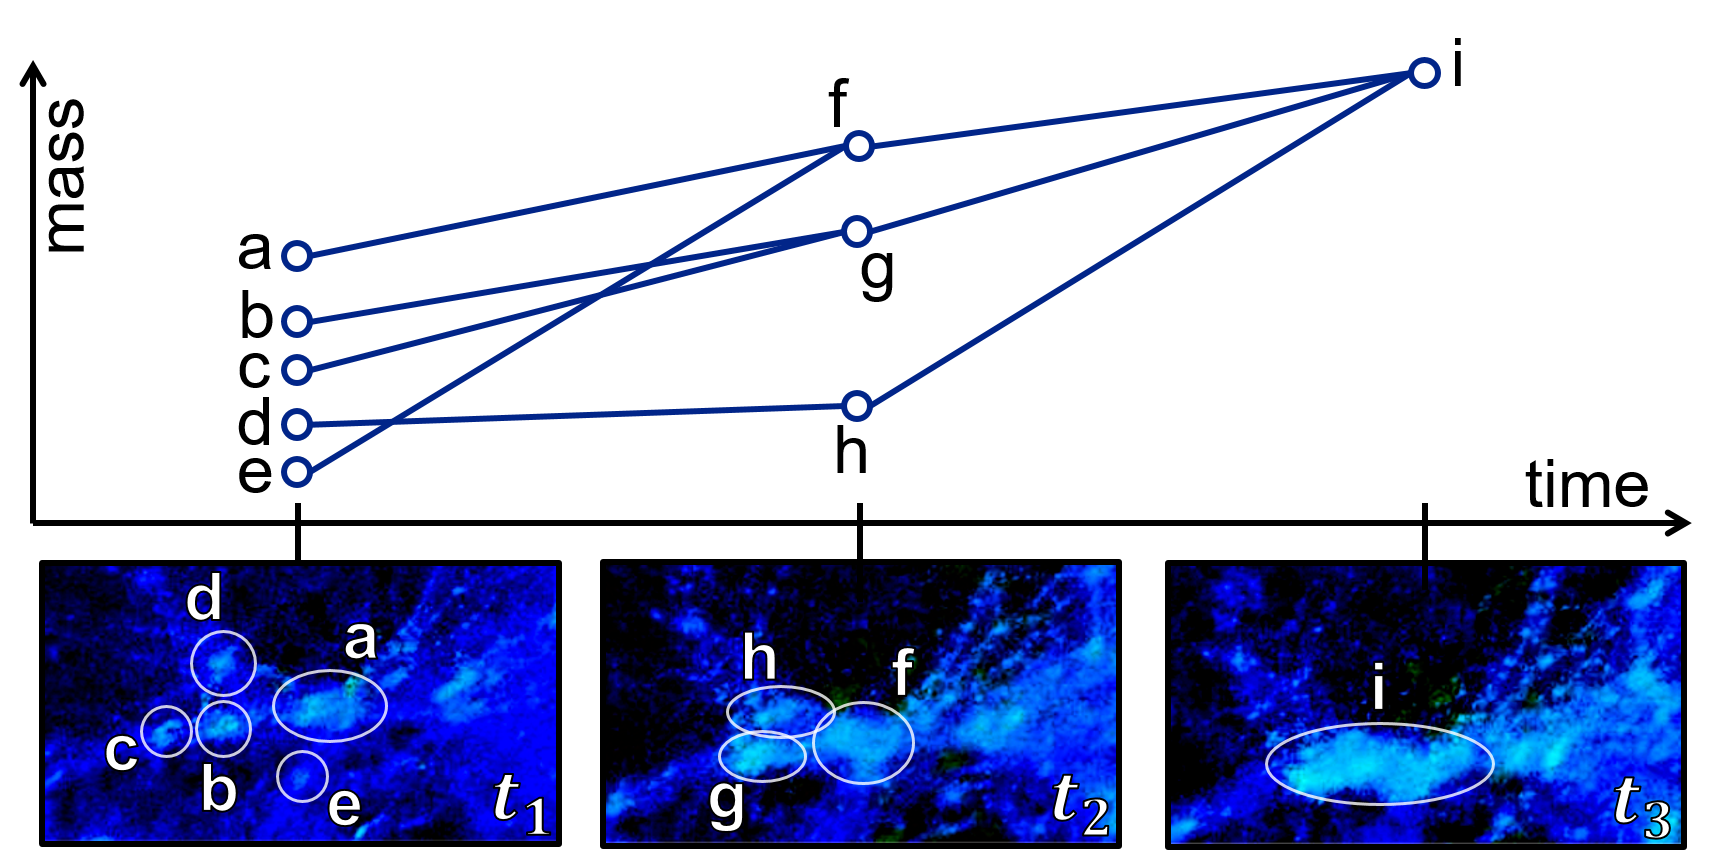
\includegraphics[width=\textwidth]{images/darkmatter/halo_explanation_4}
		\caption{The process of extracting merger trees from simulation output. Below, we see the same spatial domain at three timesteps. Over time, the particles coalesce into larger structures. A friends-of-friends algorithm identifies these groups of particles, called halos, at each timestep. The merger tree above shows halos (nodes) linked by edges which indicate the halos they merge into in subsequent timesteps.}
		\label{fig:halo_explanation}
	\end{figure}

\subsection{Merger Trees}
Once dark matter halos are extracted, they are associated across time steps to create halo merger trees~\cite{skysurvey}. These trees capture the way that halos form over time (Figure \ref{fig:halo_explanation}). The dark matter particles within encode information about the formation of structures, specifically galaxies, in the universe, a phenomenon that is currently poorly understood. Effectively visualizing the interplay between particle data, halo data, and their hierarchical evolution (as represented by a merger tree) can allow researchers to intuitively explore connections and draw conclusions.

In addition to a static visualization of halos and extracted features, researchers need to study their time-varying evolution. Shan et al.~\cite{Shan:2014} utilize a tree-like visualization view, which describes mergers linked with a 3D visualization of particle tracers to study halo evolution. In their scheme, users select halos in the 3D view, which results in the corresponding merger trees being shown in a graph layout. Our system allows selection of specific halos through the merger trees themselves, as well as using physical variables (such as velocity or mass) for laying out and organizing the merger trees. Takle et al.~\cite{Tackle:2012} developed a multilevel method of tracking the evolution and mergers of groups of dark matter tracer particles (called satellite halos) and groups of satellite halos (called host halos), visualizing these structures in isolation. Such a multilevel approach is useful since structures that interest cosmologists often occur across multiple scales. We expand upon their capability by including interactive selection as well as showing the broader context of each halo within the simulation domain.

\subsection{Visualization Techniques}
Once scientists extract features from a simulation, they can use visualization and analysis tools to explore underlying patterns in the data. One difficulty is the extensive amount of multivariate information necessary to fully represent a halo and its properties. Takle et al.~\cite{Tackle:2013} use a glyph-based representation to simultaneously visualize multiple properties of groups of halos. Another key interest lies in representing the physical shape and structure of these point-based representations. Miller et al.~\cite{Miller:2006} address this by using a unique set of 3D projections, as well as geometric glyphs showing potential correlation between galactic clusters. A visualization of the uncertainty in the simulation data is explored in a work by Haroz et al.~\cite{Haroz:2008}. Ahrens et al.~\cite{Ahrens:2006} use comparative visualization to determine subtle differences between different simulation codes using the same initial conditions. In addition, K\"{a}hler and Abel~\cite{Kaehler:2012v2} explore the use of stereoscopic techniques to enhance the perceptual ability of cosmology researchers.

There has also been an effort to generate high-quality renderings of the simulation particle data and extracted halos. K\"{a}hler et al.~\cite{Kaehler:2012} utilize a cell-projection~\cite{max1990area,Rottger2000} technique on a tetrahedral mesh derived from the initial condition of the simulation particles to visualize the dark matter density distributions; we include this method as a supplemental tool in our visualization system. Scalability becomes an issue when generating high quality images in a real-time interactive setting. Fraedrich et al.~\cite{Fraedrich:2009} use an octree based level-of-detail approach in conjunction with GPU data compression to address this problem.

In addition, there have been numerous recent advances in parallel particle rendering in general. For example, Rizzi et al.~\cite{Rizzi:2015} develop a large-scale direct point rendering framework, which uses hierarchical representations and z-ordering for improved load balancing. On the other hand, Stone et al.~\cite{Stone:2013} utilize a ray-tracing method on extracted density maps to visualize complex molecular shapes in petascale applications. In addition, Akinci et al.~\cite{Akinci:2012} use a parallel approach to surface reconstruction of large particle-based fluids based on Marching Cubes to accelerate rendering. Rendering in a distributed setting also requires careful attention to compositing techniques. One notable example, which we use here, is the 2-3 swap method developed by Yu et al.~\cite{23swap}; this efficiently and scalably performs compositing across large numbers of nodes.


\section{System Design}
 Our system design is motivated by the need to simultaneously observe multiple data types, as determined through close collaboration with domain scientists. These include particle data from the simulation, extracted halos, and constructed merger trees. An understanding of the interplay among data types is essential for scientific analysis. Moreover, visualizing the simulation's physical behavior at one timestep is more useful when associated with quantitative and chronological information. Data from the raw particles and the extracted halos inform one another; we enhance these views with both qualitative and quantitative information. Because of the scale of the data and the multitude of features, we aim to provide improved capability to focus analysis on specific features of interest. 

\subsection{System Components}
Figure~\ref{fig:system} shows our visualization system workflow. Since the raw particle data is too large to manage on a single machine, we utilize a remote parallel renderer to visualize the particles. The halo information and merger trees, however, are small enough in scale that they can be transferred to a desktop PC and visualized locally. The interactive visualization system communicates between the local file systems and the remote renderer for seamless exploration of each of the data types. The visualization tool utilizes three main views that can be used to explore the data: a particle explorer for a direct 3D rendering of particle data, a view for the exploration of merger trees, and a quantitative display for plots of halo and particle variables.

	\begin{figure}[t]
		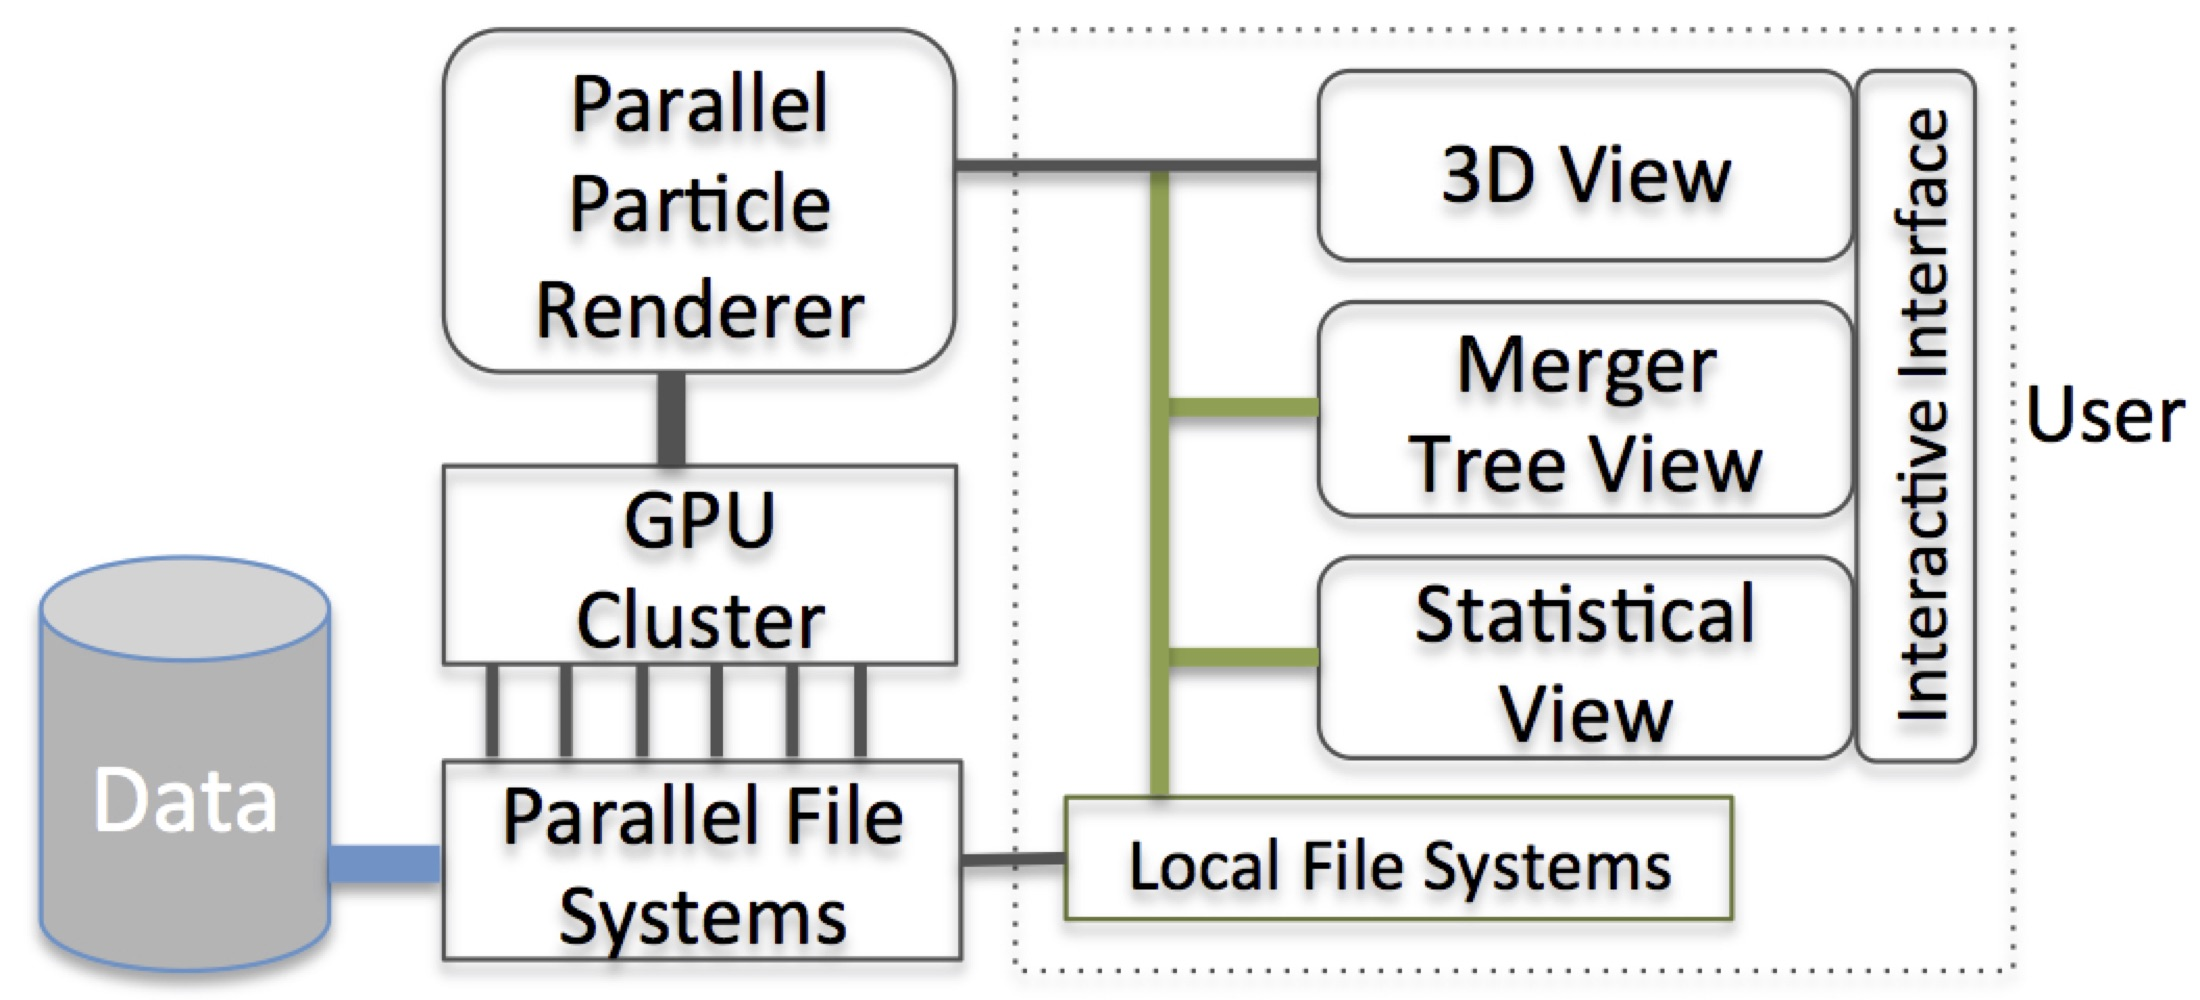
\includegraphics[width=8.5cm]{images/darkmatter/CosmoVis.jpg}
		\centering
		\caption{An overview of the system workflow. The large scale particle data resides in a distributed system and is visualized using a paralleled remote renderer. The smaller scale halo merger tree data resides locally and is rendered using a desktop computer.}
		\label{fig:system}
	\end{figure}

\subsubsection{User Interface}
The user interface (Figure~\ref{fig:ui}) integrates the three visualization tools: the quantitative and 3D particle rendering views are placed in the top right and top left respectively, with the merger tree visualization placed below. The user in this example investigates a subset of the merger trees in velocity space, choosing to view corresponding mass information in the quantitative view. Below the merger tree is a slider for selecting a particular timestep. The tabs beside the quantitative view reveal additional interface elements, such as a transfer function editor for coloring the 3D particles. Each of the views can be resized relative to the others in order to provide additional visual detail when working in that particular view.

	\begin{figure}[t]
		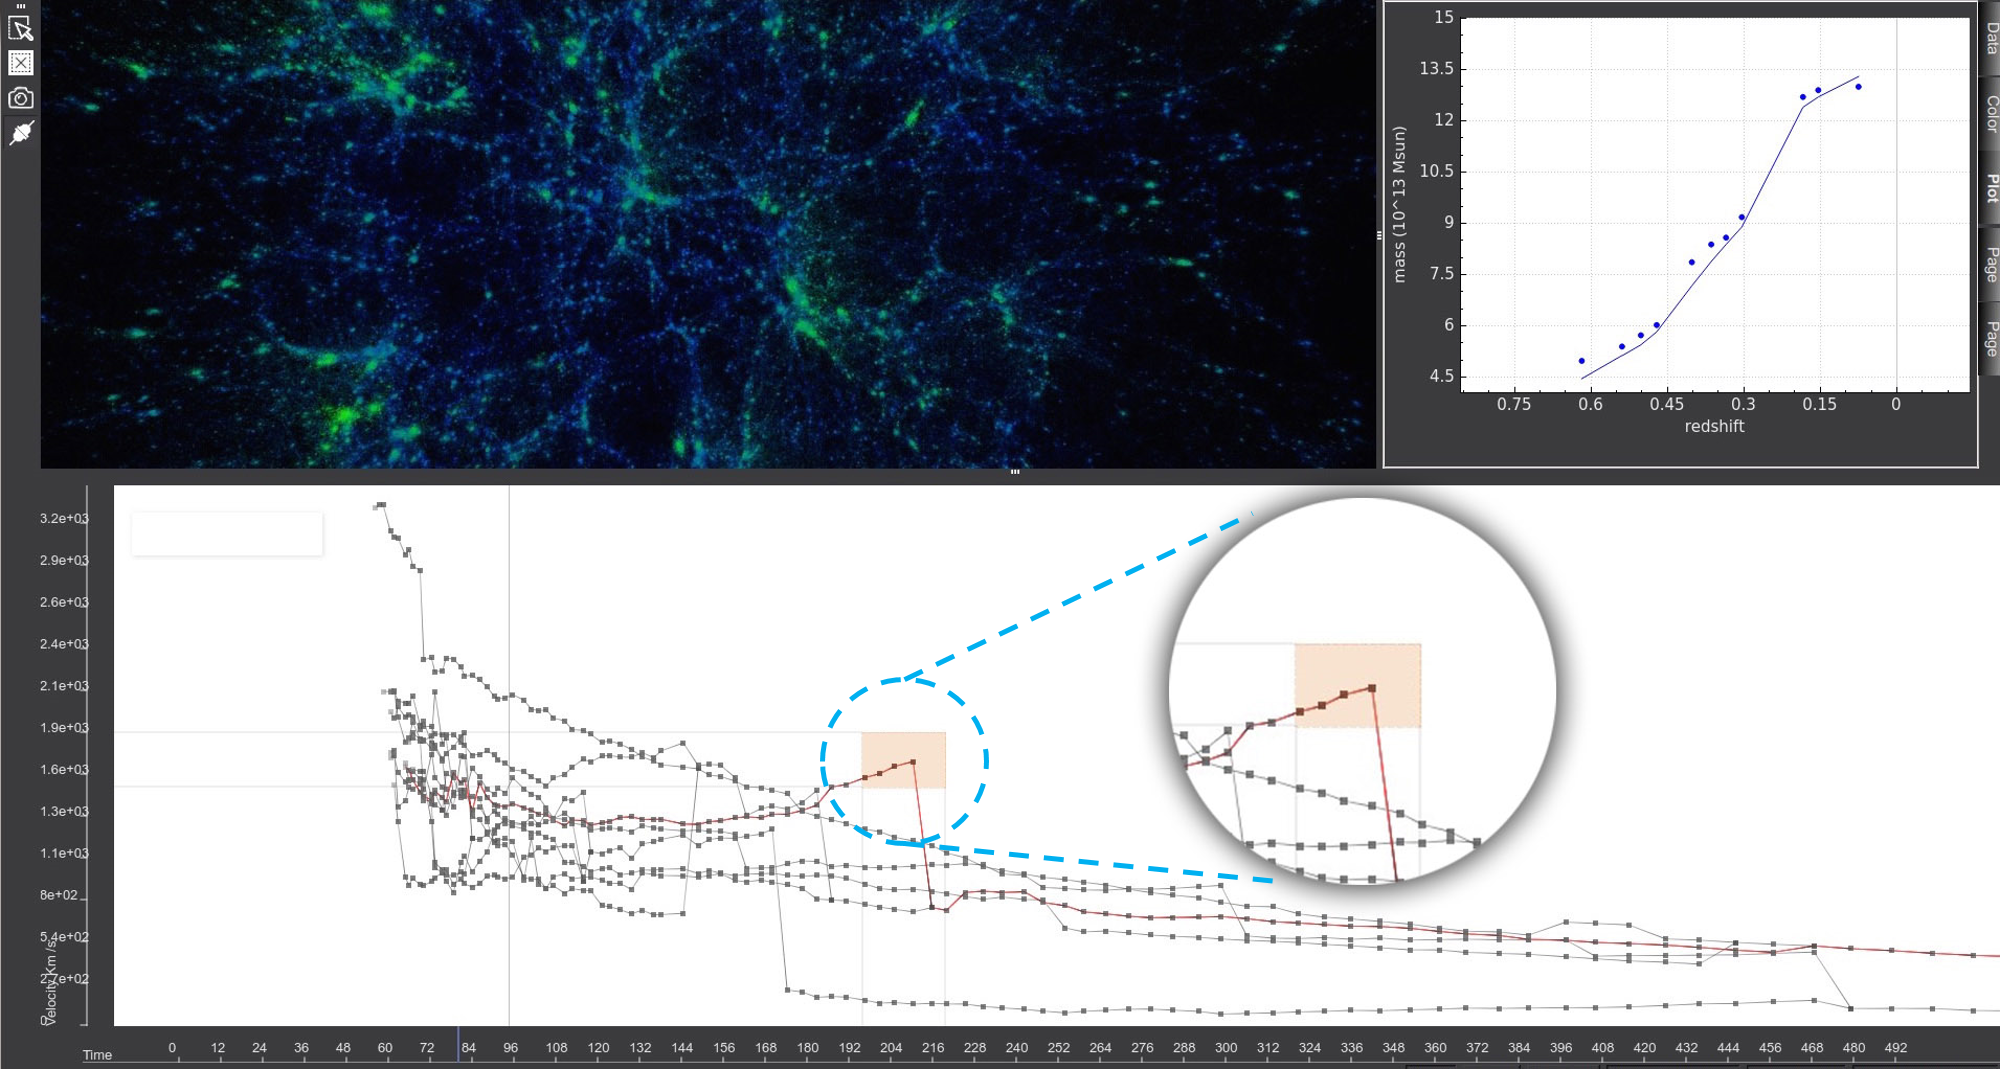
\includegraphics[width=\textwidth]{images/darkmatter/ui_new_zoomin.png}
		\caption{A snapshot of the user interface. The quantitative view and 3D particle rendering are placed on the top right and top left respectively. The merger tree visualization is placed below. Here, the user explores a subset of merger trees. For clarity in this figure, we provide a zoomed-in view of the selection box that the user has drawn.}
		\label{fig:ui}
	\end{figure}

\subsubsection{Merger Tree Visualization}
We provide an interactive visualization and selection tool for the halo merger trees, which are hierarchical representations of the dark matter halo formation histories. Each halo present in the final timestep of the simulation has an associated merger tree describing its past. On average, there is approximately one halo for every thousand particles in the final timestep of the simulation. Given this data size, viewing all the trees simultaneously would not allow for detailed visual analysis of the mergers due to overplotting and clutter. We employ several methods for reducing the number of trees needed for visualization. The user can focus on a single merger tree, progressing through the data one tree at a time. We also provide capability to iteratively select smaller subsets of trees using selection boxes and zooming. Another approach uses lists of interesting halo events that domain scientists identify in postprocessing in order to select a tree or trees of interest. Scientists are particularly interested in merger trees that do not behave as expected; these trees might be reflective of bugs in the halo finder code. For example, a massive halo that suddenly appears in one timestep is not physically feasible, since it must coalesce over time from a mass close to the simulation's minimum mass resolution. We offer the option to select and isolate merger trees based on these anomalous events. Because there are far fewer halos than particles, we can store and visualize the merger tree data at an interactive rate using a local desktop computer.

	\begin{figure}[t]
		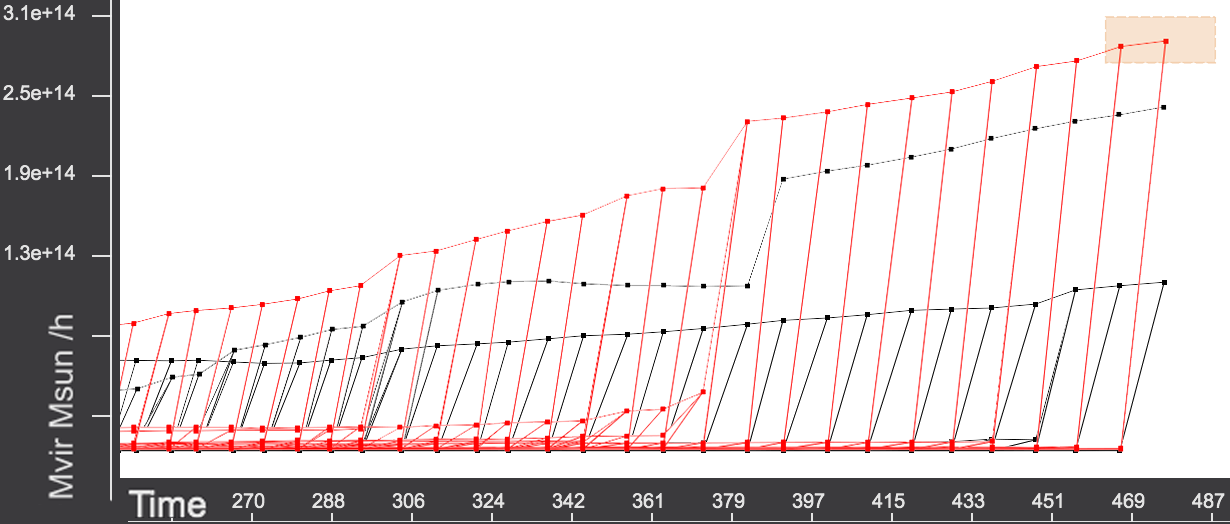
\includegraphics[width=\textwidth]{images/darkmatter/mt_overview.png}
		\caption{Several merger trees (black) with time on the x axis and mass on the y axis. The user chooses a node with the selection box, which highlights all progenitors and descendants leading to and from that node (red). Large vertical jumps represent nodes at which a halo was subsumed into a much larger halo due to gravitational force.}
		\label{fig:mergetreehundred}
	\end{figure}

The merger tree visualization draws the tree structures and allows for interactive exploration (Figure~\ref{fig:mergetreehundred}). While the horizontal axis represents time by default, since temporal evolution is of primary importance, both axes can be mapped to any halo-specific property of interest (e.g., mass or velocity). In addition, our system offers zooming and selection capabilities; the zoom reduces the visible range of timesteps or of the mapped property, while the selection feature allows for highlighting of particular trees or descendant node families. The selection is highlighted and corresponding particle IDs are communicated to the remote particle renderer so that the particles belonging to the selected halos/nodes can be highlighted in 3D space. Lastly, mousing over portions of the merger tree will display additional relevant information for that particular node.

\subsubsection{3D Rendering}
This view offers context for the data extracted by the halo finder and merger tree code. A 3D view of the simulation particles shows the physical behavior of the system in an intuitive way. This is useful, for example, when inspecting a halo that behaves strangely in the merger tree, such as one that suddenly appears well above the simulation mass resolution. A view of the corresponding merger tree will simply show that such a halo appears, providing little further information. However, a 3D interactive view of the particles over a range of sequential timesteps may inform the user that something else is happening in the interplay between the simulation and halo finder code. In this situation, a halo may split into two halos in a subsequent timestep, potentially leaving one of the massive resulting halos without a progenitor. A view of the particles reveals this information where the merger tree code and other quantitative information may not.

We make the particle view fully interactive. Users can control various settings the view using standard camera controls (rotate, zoom, pan, etc.) or the color mapping using a transfer function editor. Figure~\ref{fig:variance_comparison} shows an example of particles colored according to their velocity (right) vs. particles colored according to their variance with the local velocity field (left), as in \cite{Popov:2011}. We can see that particles with higher velocities and particles with higher variances, or differences with their local velocity fields that may indicate structure formation, tend to occupy space near the centers of clusters and halos.

In addition, users can manually select interesting groups of particles. We employ a two-step process to select particles in 3D space on the 2D screen-space projection. Users first select particles from one viewing angle of interest using a box selection tool. This defines a view frustum that extends infinitely away from the screen. Next, users adjust the length of this frustum from an orthogonal viewing angle to finalize the selection area. Any particles/halos that are selected in this view are correspondingly selected in all other views as well.

%	\begin{figure}[t]
%		\includegraphics[width=8.5cm]{all_particles.png}
%		\caption{The particle renderer depicts about one billion particles for each timestep using particle splatting. In this image, color is mapped to velocity magnitude with faster particles in green. The simulation represents a cube with sides of 256 Mpc, or about 800 million light years.}
%		\label{fig:rendering}
%	\end{figure}
	
	\begin{figure}[t]
		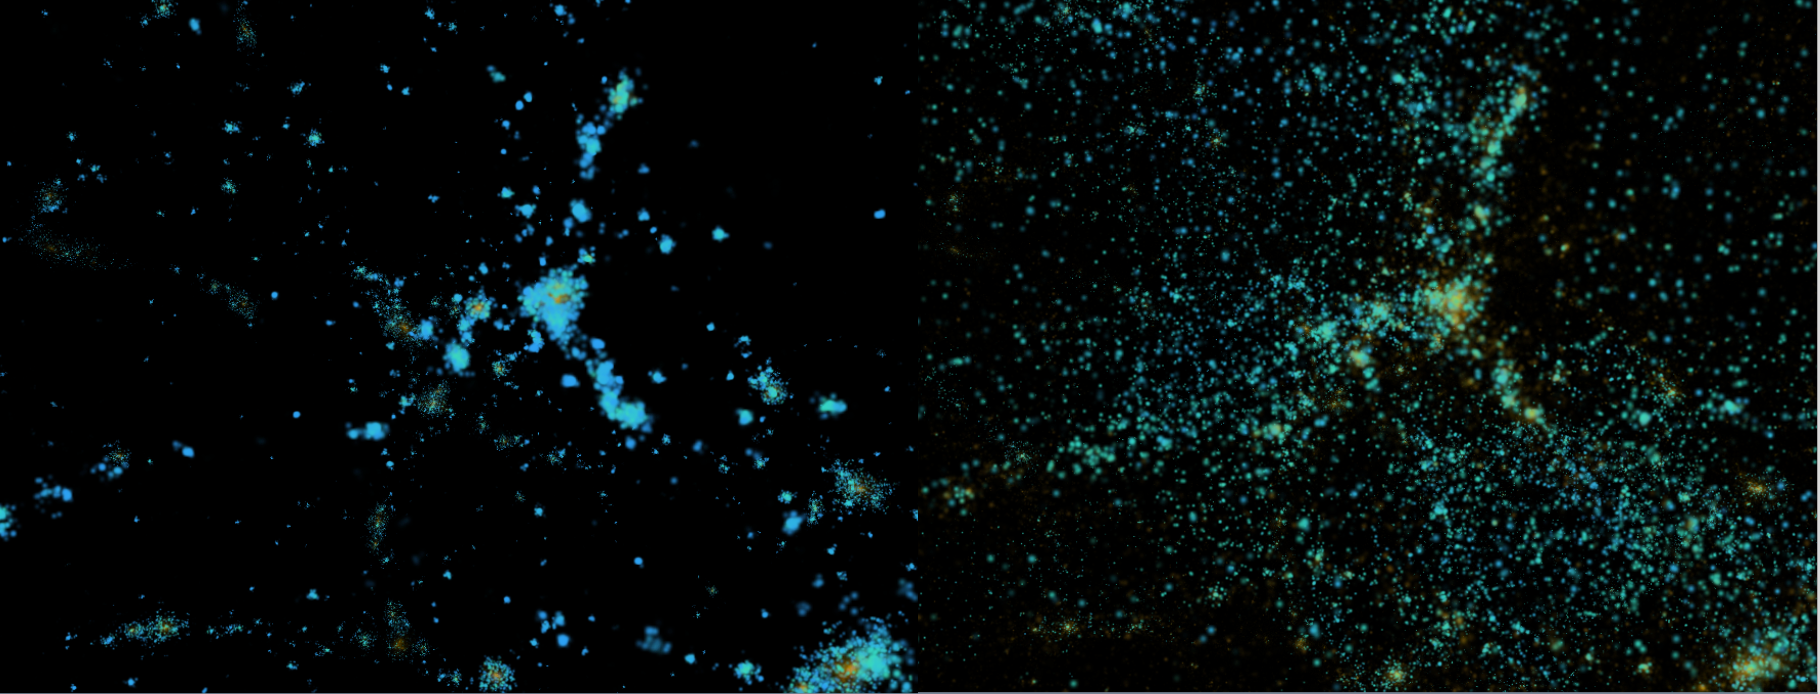
\includegraphics[width=\textwidth]{images/darkmatter/variance_comparison.png}
		\caption{Comparison of different color mappings on particles. Right) Mapping the velocity of the particle. Left) Mapping the variance with the local velocity field. Blue indicates smaller values while green/yellow indicates larger ones.}
		\label{fig:variance_comparison}
	\end{figure}
	
Producing such a view, given the number of particles in each timestep ($\sim 1$ billion), introduces several challenges. First, the user must be able to explore at interactive speeds in order to gain an intuitive understanding of the particle behavior. Second, the merger trees selected by the user may be quite spatially distant from one another, so the entire spatial extent of the domain must be rendered in order to accommodate such requests. Rendering the entire domain also gives crucial global context for areas of interest. To meet these challenges, we incorporate a parallelized particle renderer using a remote server. The rendering server is designed to run on a large visualization cluster and handle data sizes that would be infeasible to render on a single desktop.

\begin{figure}[t]
\begin{center}
$\begin{array}{c}
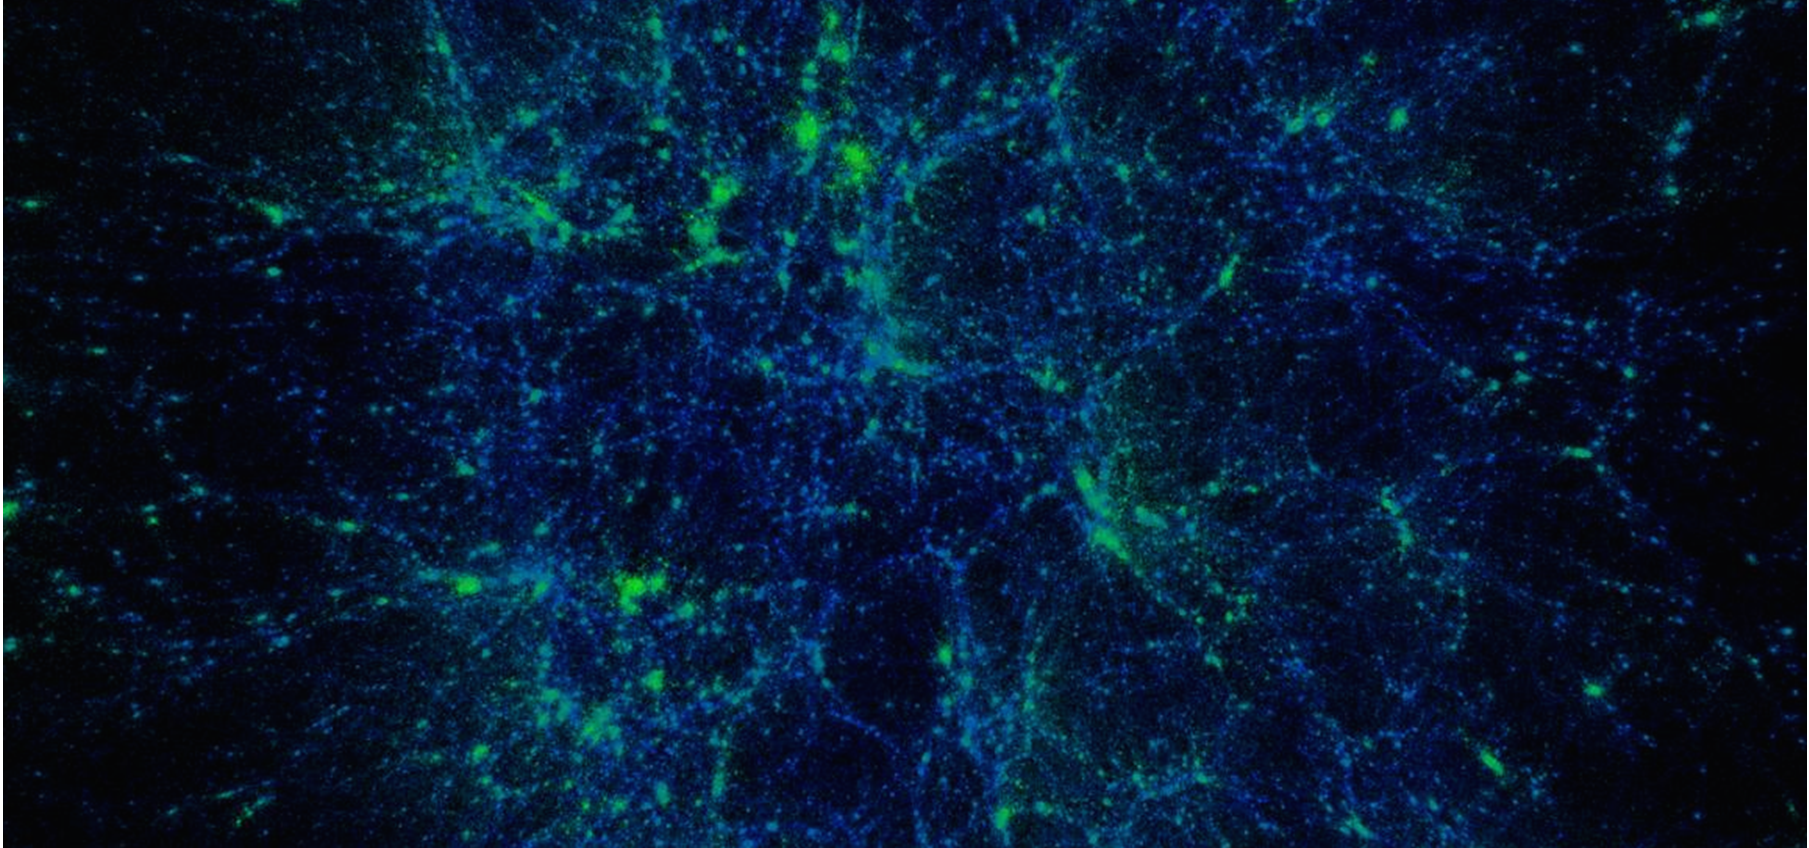
\includegraphics[width=0.95\linewidth]{images/darkmatter/rendering_comparison_b.png}
\vspace{-.05in}
\\
\mbox{\small{(a)}}
\\
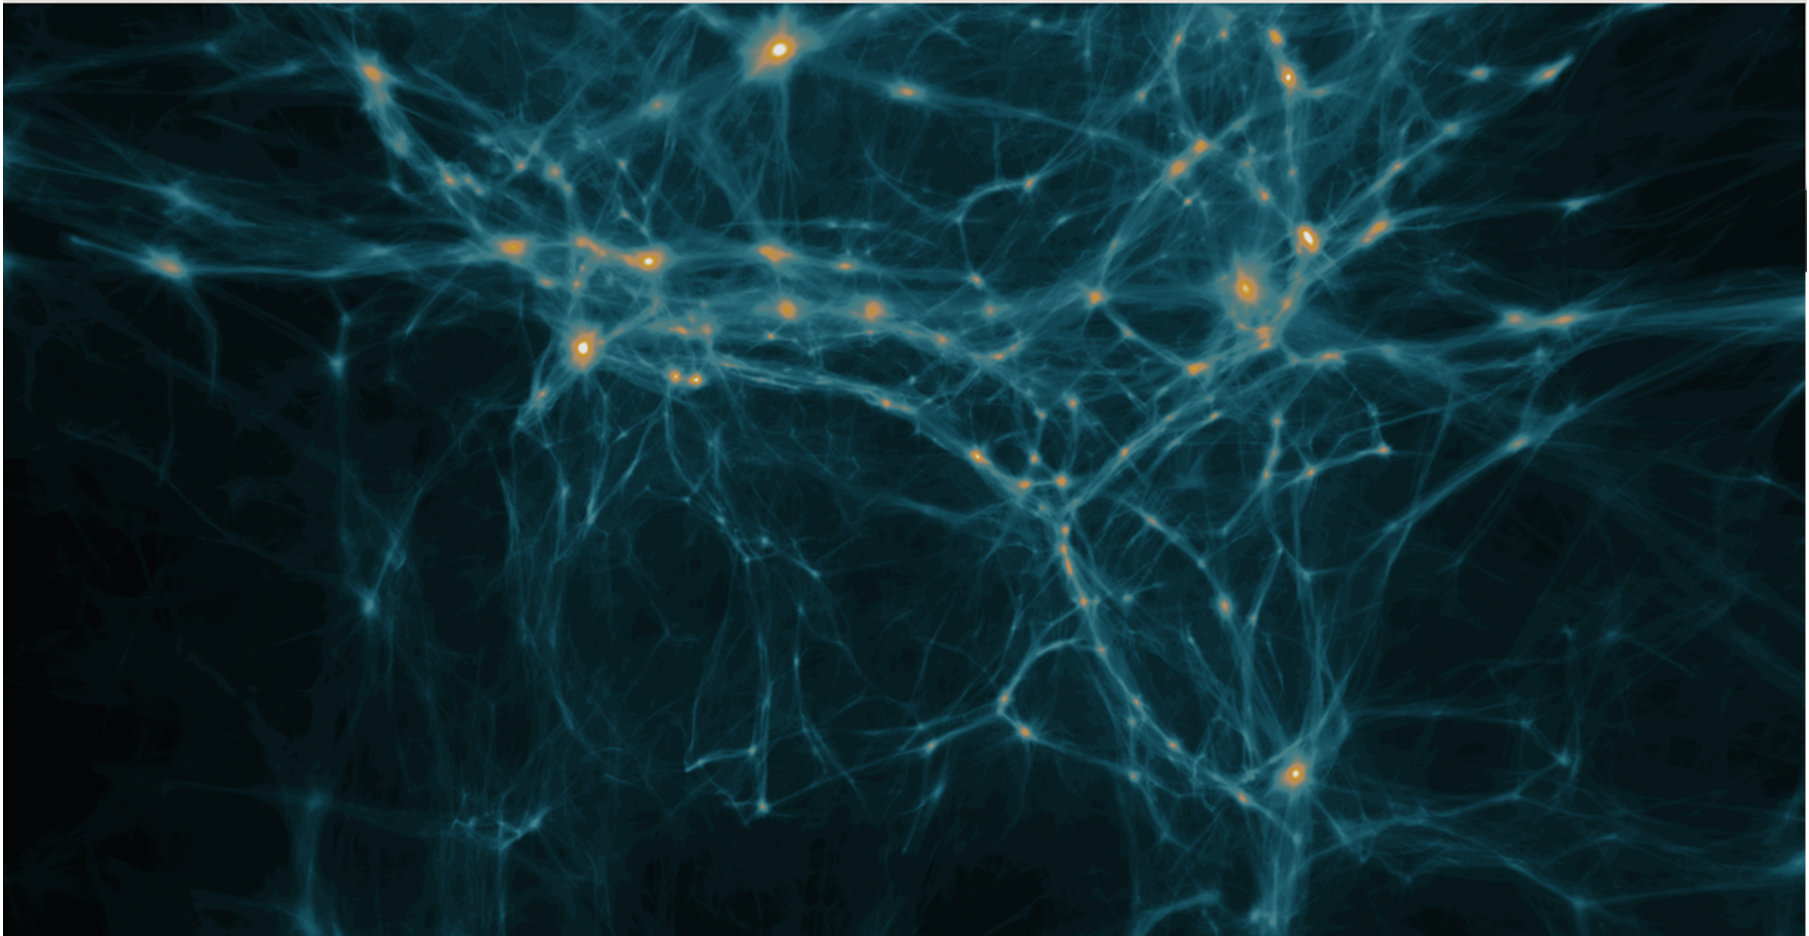
\includegraphics[width=0.95\linewidth]{images/darkmatter/rendering_comparison_a.png}
\vspace{-.05in}
\\
\mbox{\small{(b)}}
\end{array}$
\end{center}
\vspace{-.2in}
\caption{The default particle-based rendering, (a), in comparison with the alternate rendering technique, (b). The default particle view directly conveys data from the simulation, illuminating simulation and analysis code behavior. The alternate technique offers stronger depth cues as well as further insight into the structure of voids and filaments present in the universe.}
\label{fig:comparison_figure}
\end{figure}

In addition to the point-based renderer described above, we also provide an alternate way of visually representing the simulation data. While the point-based approach is useful for visualizing the individual particle locations and distributions when exploring halo substructure, it does not easily portray the filament-like structures that are present in a more macroscopic overview of the data. To address this, we implement another rendering method, which uses a tetrahedral mesh ~\cite{Kaehler:2012}, and allow users to switch between rendering techniques as necessary (Figure~\ref{fig:comparison_figure}).

The main advantage of this technique is that the filament-like structures between larger clusters of matter become obvious to the viewer. One major inaccuracy with N-body simulations comes from the assumption that particles represent a spherical kernel of mass distribution, leading to an exaggeration of gravitational attraction. This may generate extra clumping of particles which compounds on itself as the simulation progresses. The tetrahedral mesh rendering helps to alleviate these inaccuracies through a continuous density approximation of 3D scattered points~\cite{bachthaler2008continuous} and is especially useful in the filament regions. However, this technique is secondary in usefulness to the particle representation, which is directly representative of the data in the simulation and conveys how particles are grouped into halos. Therefore, we use particle splatting as the default method and offer the tetrahedral mesh method as an alternative when desired.

\subsubsection{Quantitative View}
In order to provide quantitative analysis as a complement to the qualitative features of the other views, we incorporate a plot viewer, which utilizes the QCustomPlot library \cite{QCustomPlot}. We employ this view for several specific applications, each extending the usefulness of the two other views with additional quantitative information.

\begin{figure}[t]
        \begin{subfigure}{0.5\textwidth}
        \centering
         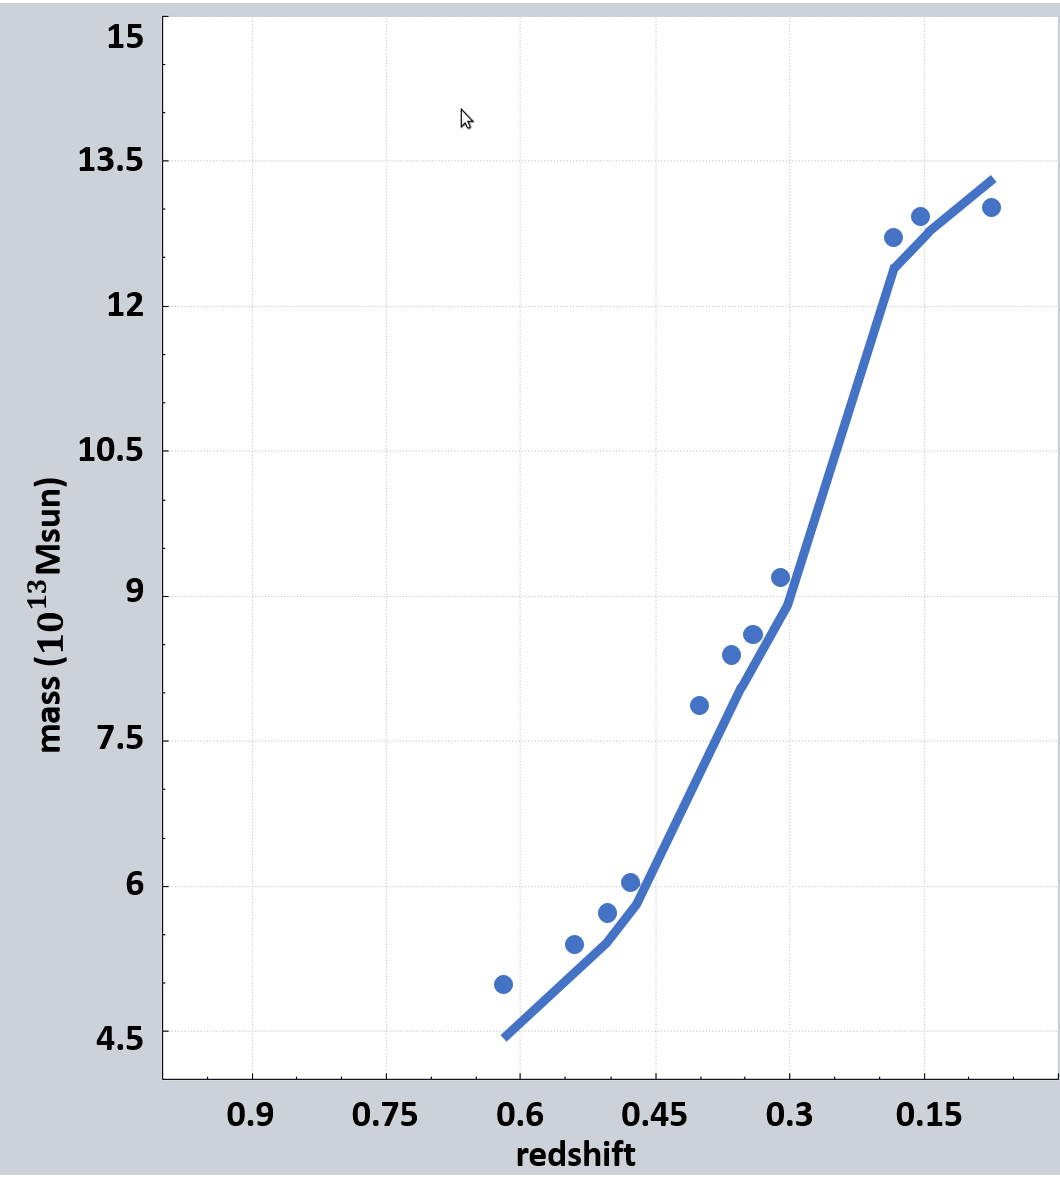
\includegraphics[width=\textwidth]{images/darkmatter/new_plotview_left.png}
                \caption{}
                \label{fig:MPs}
        \end{subfigure}%
        \begin{subfigure}{0.5\textwidth}
        \centering                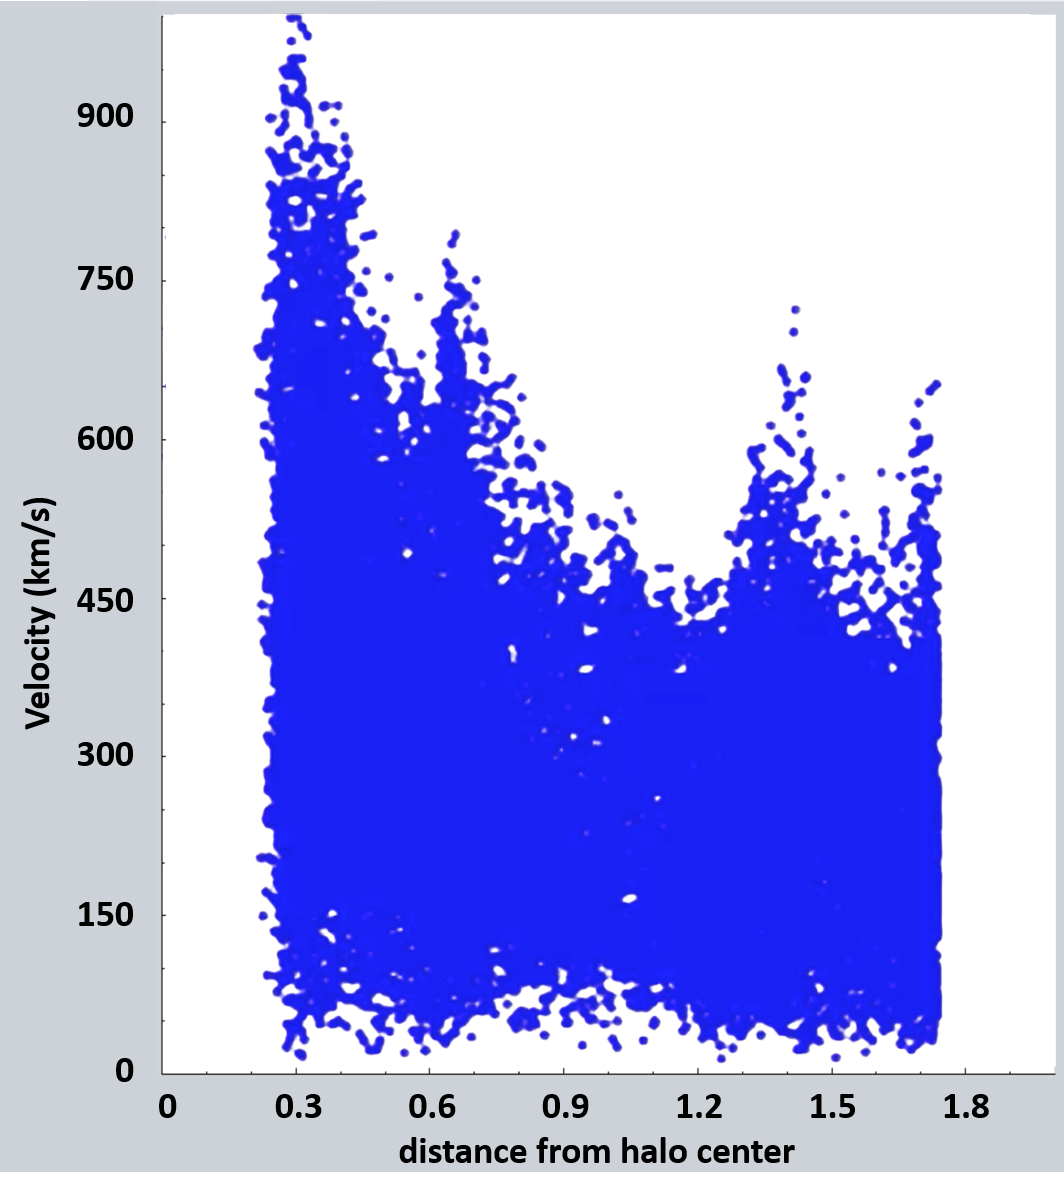
\includegraphics[width=\textwidth]{images/darkmatter/fixed_plotview_right.png}
        \caption{}
        \label{fig:velocity}
    \end{subfigure}
        \caption{The plot view can provides quantitative feedback based on the user's selection in one of the other view spaces. This can reflect selection of a tree in the merger tree view (a), or of a halo in 3D space (b). The left side contains a plot of the missed progenitor history for a selected merger tree. The dots represent anomalous halos; the solid line reflects the sum of the corresponding progenitors. On the right, we plot velocity magnitude vs. distance from halo center, in simulation coordinates, for particles near a selected halo. This local velocity information provides intuition for how the halo is forming; peaks in the plot may indicate substructure.}\label{fig:plots}
\end{figure}

One option given to the user is to view a chronological plot of the anomalous events in a particular halo's history. The system can automatically find instances of events, such as missed progenitors, subject to a user's input threshold. An example of such a plot is shown in Figure~\ref{fig:MPs};  here, a user chooses to locate all nodes for which the sum of the progenitor masses differ from the halo mass by more than $5 \times 10^{12}$ solar masses. Seeing these events chronologically, as well as a quantitative assessment, guides selection for further exploration in the merger tree view.

The user can also choose to see quantitative information about the particles that make up a selected halo. This halo may be selected from the merger tree view or the 3D view. Plotting velocity versus distance from halo center, as the example in Figure~\ref{fig:velocity}, provides additional information about the halo's behavior that is not apparent in the merger tree or 3D views. Such a plot highlights the difference between a stably rotating halo and one in the process of violent mergers. A stable halo should have a relatively continuous velocity distribution, while subhalos interacting with one another will lead to spatially distinct peaks in velocity. This information provides scientists with additional clues as to how structures, such as galaxy clusters, could form in that location.

\subsection{Implementation Details}
The merger trees contain a node for each halo, as well as edges connecting halos with their progenitor and descendant halos. The system reads locally available data, which specifies ID numbers for each halo and its progenitors, and calculates the corresponding tree. This short preprocessing task occurs when the dataset is first loaded.

Our parallel particle renderer performs four steps: data partitioning and loading, local particle splatting, compositing, and sending the resultant image to the client. The data is partitioned into spatially contiguous chunks according to an even subdivision of the particle domain. Although the particle data can be sparse (particularly in later timesteps when dark matter particles have coalesced), it is fairly uniformly distributed for much of the simulation, such that a relatively coarse partitioning with one chunk of particles per rank tends to produce an even load across all ranks. Each chunk is rendered locally on the GPU by splatting its particles to the screen as partially transparent disks~\cite{Gumhold:2003} and blending accordingly. The data chunks are organized into a spatial subdivision tree for easy sorting in view order, and compositing is handled by the 2-3 Swap parallel compositing algorithm~\cite{23swap}. After compositing, the final image is compressed on the head node before being sent over the network to the visualization client. Additional communication between the client and server transmits interactive settings, such as particle selections or color mapping, whenever their values change.

The alternative rendering approach works by treating individual particle locations as vertices of a tetrahedral mesh that is computed in the first timestep of the data. This can be easily determined since the particles are evenly distributed on a near regular grid fashion at the initial condition of the simulation. As the simulation progresses, the tetrahedral mesh becomes deformed as particles move throughout the domain by their gravitational pull and coalesce into halos and larger clusters. These tetrahedra are projected into screen space and are accumulated per pixel to generate an estimate of density in that region. A comparison between this alternate technique and the original point-based method can be seen in Figure~\ref{fig:comparison_figure}.


\section{User Feedback and Results}

We assess our system using data from the Planck simulation run of the HACC framework. This dataset contains 100 timesteps with 1 billion particles ($\sim30$ GB) per timestep. While larger datasets exist, this particular simulation uses a particularly fine mass resolution in order to explore dark matter halo activity in detail. The time ranges from a redshift of $z = 10$ to $z = 0$, which roughly corresponds to 500 million years since the Big Bang, to the present day, about 14 billion years since the Big Bang. The spatial range of the simulation is a cube with sides that are 256 Mpc ($\sim 800$ million light years) in length. This wide temporal and spatial window is important for an accurate simulation, especially because the nature of dark matter and structure formation are largely unknown; scientists cannot safely make assumptions concerning their behavior without simulation data. The merger tree data consists of about 400,000 trees, each representing the evolution of a different halo.

We have consulted closely with several domain scientists, who work with HACC at Argonne National Laboratory, to assess the usefulness of our tool. In general, cosmology researchers are interested in highlighting a specific halo, retrieving relevant information such as its mass, position, or velocity, and tracking descendants and progenitors. The scientists have emphasized that in order to unearth the cause of anomalous merger tree events, it is sometimes necessary to look at how individual halo nodes interact with one another over several consecutive time steps. Thus, our capability for seeing how the halos physically join and split is very useful. When a feature-tracking algorithm returns unpredicted values, numerical analysis alone may not reveal the underlying cause and whether it is a physically feasible event or a feature of the code that needs to be refined. This is especially troublesome because the definitions of mergers, halos, subhalos, and other extracted features may be quite ill-defined. Observing case studies of anomalous events, and seeing the integrated merger tree, quantitative, and 3D views, helps scientists develop and test a hypothesis as to why the simulation data seem to be behaving contrary to physical laws, or to develop an intuition beyond a single numerical model. In addition, our integrated comparison features are useful for data that do not seem to be anomalous. Comparing merger trees for a single halo generated with two different codes, for example, helps qualitatively verify that the outcomes are correct. 

\subsection{Case Studies}

A rigorous definition of a dark matter halo, and the best algorithmic solutions for finding halos and identifying their merger trees, are open-ended areas of active research~\cite{Knebe:2011}. The choice of halo finding algorithm may give inconsistent results or misidentify the behavior of dark matter. To investigate this issue, domain scientists are interested in exploring anomalous nodes in merger trees. These events provide information for further refinement and perfection of their analysis codes. In turn, this visual diagnostic and refinement process will improve the analysis available for large observational surveys such as LSST~\cite{LSST}.

\subsubsection{Heavy Birth Events}

One feature of merger trees that is unreflective of physical laws in reality is the sudden appearance of halos that are well above the simulation's mass resolution. Such an event is unphysical because the particles begin as discrete objects and halo mass must increase continuously over time. This may be caused when a large halo splits into two separate components, such that one of the resulting pieces is identified as having a progenitor and one is not. These scenarios are easy to locate analytically, but it is more challenging to characterize the cause for all of these ``heavy birth'' events. Our linked views provide a way to qualitatively assess such events, verify hypotheses for the inconsistent results, and iteratively refine merger tree code to incorporate this information. The user may see the indication of a heavy birth event in the plot view, select the corresponding node in the merger tree view (Figure~\ref{fig:heavy_birth1}), then refer to the 3D view (Figure~\ref{fig:heavy_birth2}) for information as to why the halo merger code detected an anomalous event. The left side of Figure~\ref{fig:heavy_birth2} shows a ``heavy birth'' halo, and the right side shows this halo in the next timestep, where the halo finder identifies three distinct groups as being in the same halo.

	\begin{figure}[t]
		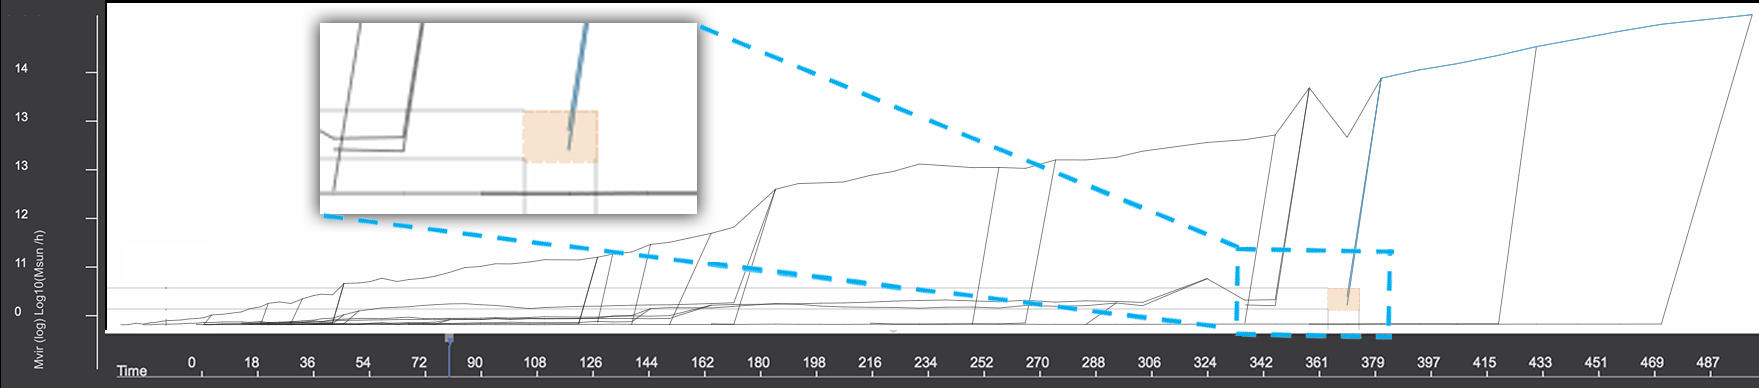
\includegraphics[width=\textwidth]{images/darkmatter/heavy_birth.png}
		\caption{In the merger tree view, the user selects a node with no progenitors that is much more massive than the simulation resolution. This selection triggers highlighting of the relevant particles in the 3D view, seen in this figured in the zoomed-in box.}
		\label{fig:heavy_birth1}
	\end{figure}

	\begin{figure}[t]
		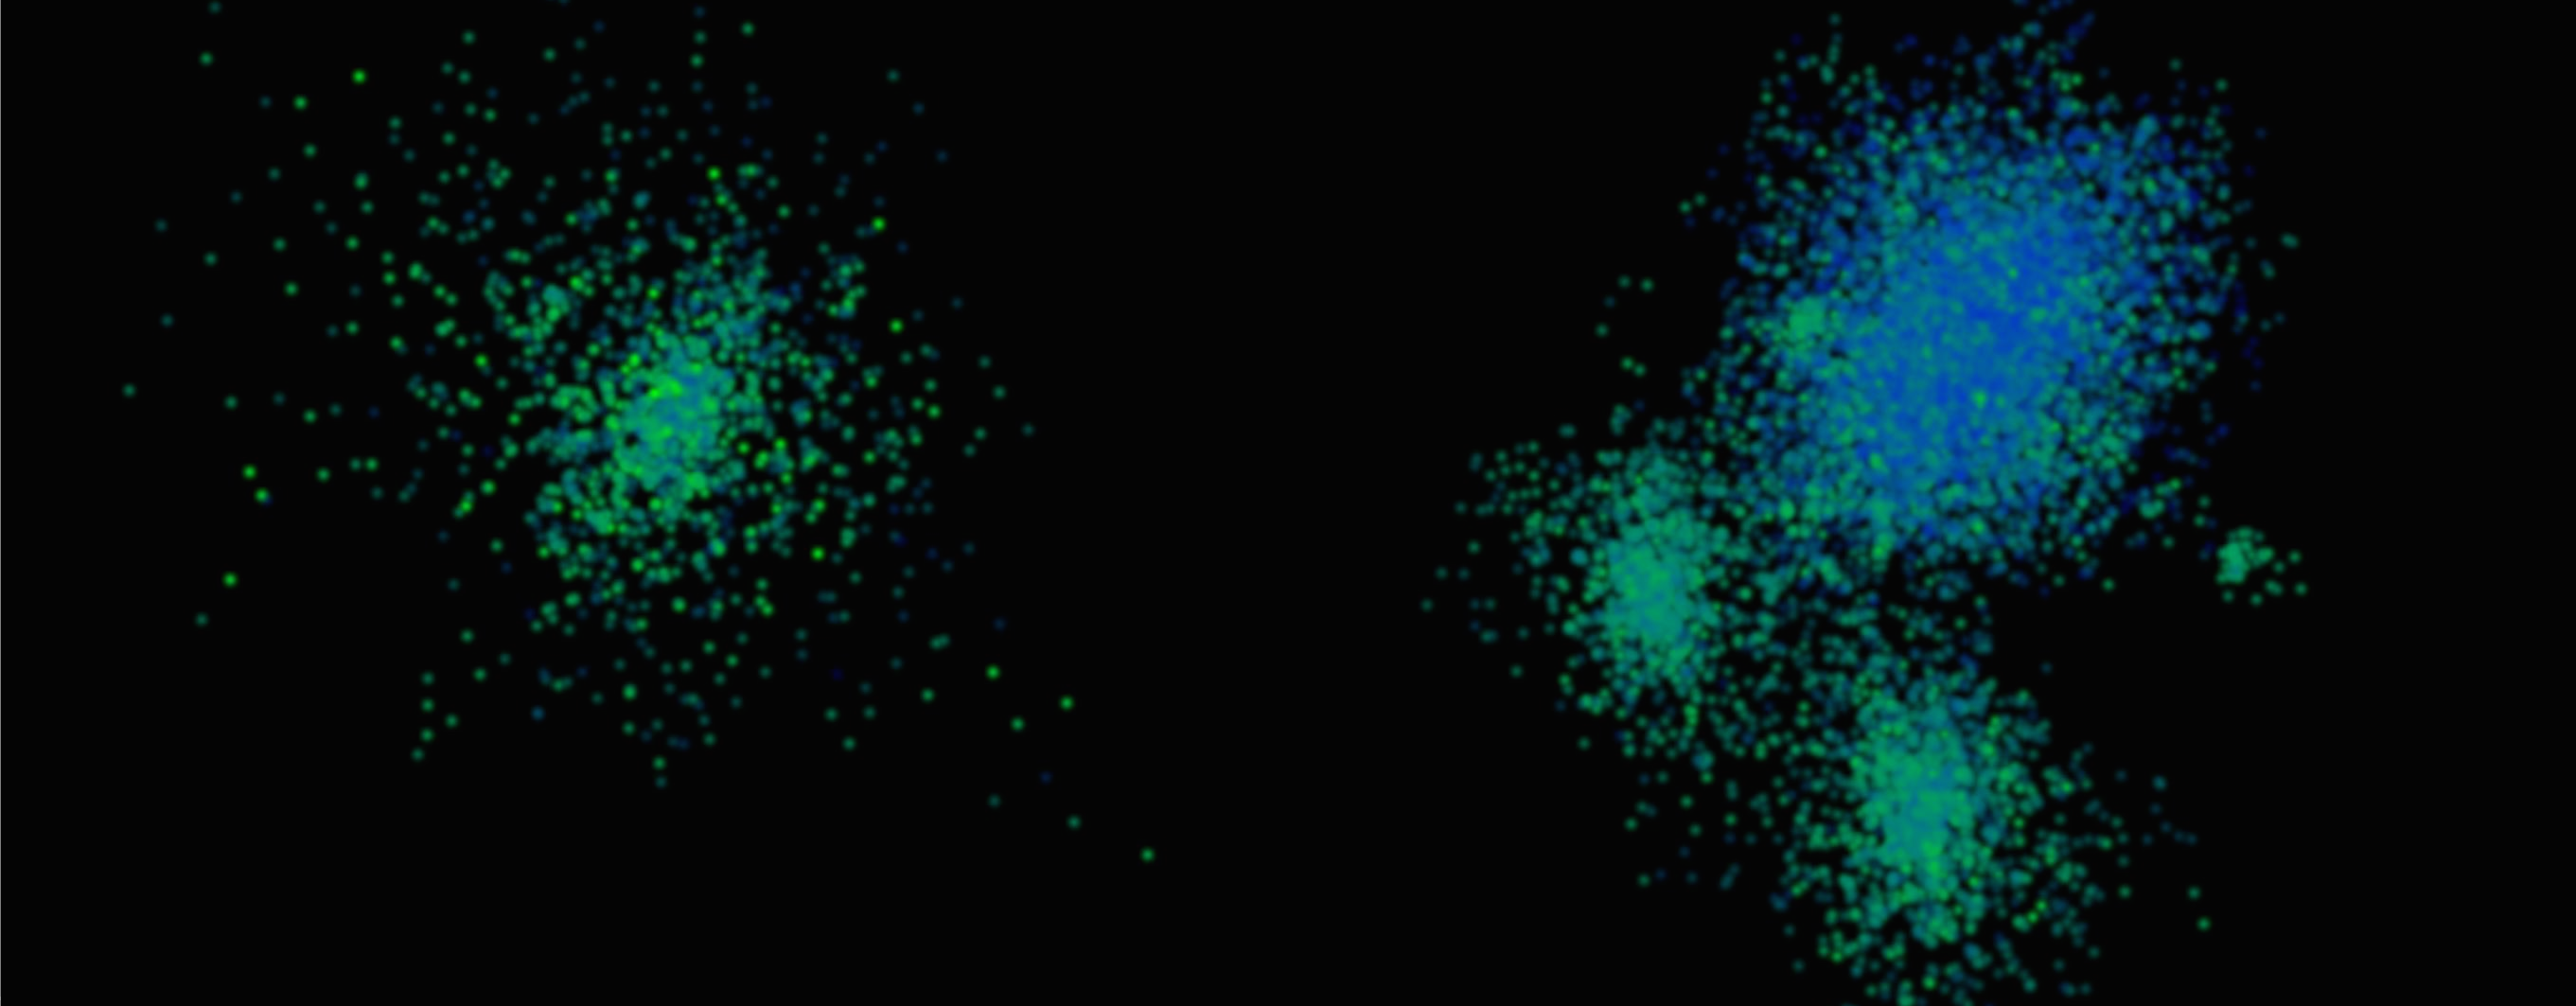
\includegraphics[width=\textwidth]{images/darkmatter/hb_particles.png}
		\caption{Particle data for the selected heavy birth in Figure~\ref{fig:heavy_birth1}. The left image shows the selected halo while the right image shows the same halo a few timesteps later. Note the two satellite halos to the bottom left of the host halo; the halo detection algorithm determines that the halo subsequently grows to include several smaller structures.}
		\label{fig:heavy_birth2}
	\end{figure}

\subsubsection{Missed Progenitors}

The merger tree code may also incorrectly identify a halo and group of progenitors in such a way that the sum of the progenitors' masses differs from the resulting halo's mass by an amount much greater than the simulation's mass resolution. In most of these cases, the total mass of progenitors is less than the halo mass, indicating that one or more halos has been missed by the detection code. 

In the example shown earlier (Figure~\ref{fig:MPs}), the mass of all known progenitors (drawn using a solid line) is noticeably lower than the mass of the resulting halo (drawn as dots) in many timesteps. Moreover, we can see that the mass of the progenitors tends to periodically catch up to the mass of the resulting halo (at $z = 0.45, 0.3, 0.15$ in this case). This pattern could indicate that this merger tree experiences many interactions with other halos. For example, a halo might split apart because of a gravitational interaction, and one resulting piece may join another tree, an event that is difficult to simply characterize using a halo-matching algorithm. In addition, we find that the last timestep results in a halo mass that is less than the sum of its progenitors. Unlike the previous timesteps, the detection code seems to have either identified too many progenitors, or misidentified some heavy halos as progenitors.

%	\begin{figure}[t]
%	\centering
%		\includegraphics[width=3cm]{mp_432.png}
%		\caption{The particles corresponding to the halo represented in Figure~\ref{fig:MPs}. Complex substructure hints at the reason for inconsistent behavior of the halo finding algorithm.}
%		\label{fig:MP_part}
%	\end{figure}

%Figure~\ref{fig:MP_part} shows the corresponding particle data for the halo in question. 
%The high density of particles in this halo coupled with its complex structure could reveal the cause of the discrepancy; perhaps a subhalo is inconsistently being labeled by the code as contained or not contained within the host halo. 

Viewing the corresponding particle data for the halo in question could reveal the cause of the discrepancies; perhaps it contains a subhalo that is inconsistently being labeled by teh code as contained or not contained within the host halo. As with the heavy births, identifying the occurrences of these missed progenitors and further exploring their properties in all three views is essential in correcting and improving merger tree codes. 

\subsubsection{Tidal Disruptions}

After dark matter halos form, they are still subject to gravitational forces from surrounding halos; this may lead to a halo being tidally ripped apart, its particles dispersing in subsequent timesteps. Missed progenitor events, above, may be related to these disruptions. Though such disruptions are certainly physically possible, they are impossible to represent using the current tree structures in which the number of nodes in a tree only becomes smaller over time. Domain scientists are interested in refining their data extraction techniques to take these events into account. Figure~\ref{fig:disruption} shows an example of a tidal disruption candidate that was identified in a preprocessing step. Because one merger tree is inadequate for capturing this event, a user may select nearby halos in the 3D view and inspect their corresponding merger histories or other quantitative information. Through this iterative process, the user can understand how tidal disruptions are characterized in the merger tree framework. The scientists we consulted with are interested in this analysis capability as a basis for developing a new merger tree model that can incorporate halo disruptions.

	\begin{figure}[t]
		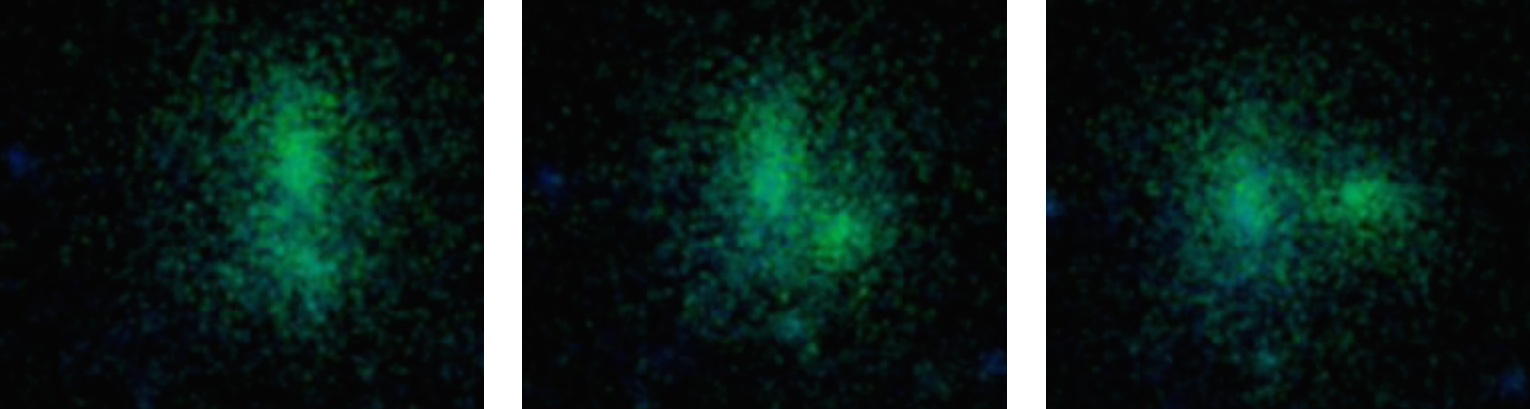
\includegraphics[width=\textwidth]{images/darkmatter/disruption_final.png}
		\caption{Three consecutive snaphsots at late timesteps of a halo that may be experiencing tidal disruption. This is visible in the group of particles that becomes distinct from the host halo over time.}
		\label{fig:disruption}
	\end{figure}

\subsection{Comparative Visualization}

Our system also facilitates visual comparison among data generated using different parameters through a snapshot functionality. Halo finding can be performed with various parameters: for example, the minimum number of particles required to form a halo. In this particular dataset, two sets of merger trees were generated, one with a 10-particle per halo minimum and one with a 100-particle per halo minimum. Figure~\ref{fig:10vs100} compares 10-particle minimum and 100-particle minimum merger trees for the same halo with mass mapped to the vertical axis. The user may choose to save two or more merger trees for comparison in this way, possibly with the corresponding 3D views or quantitative data.

	\begin{figure}[t]
		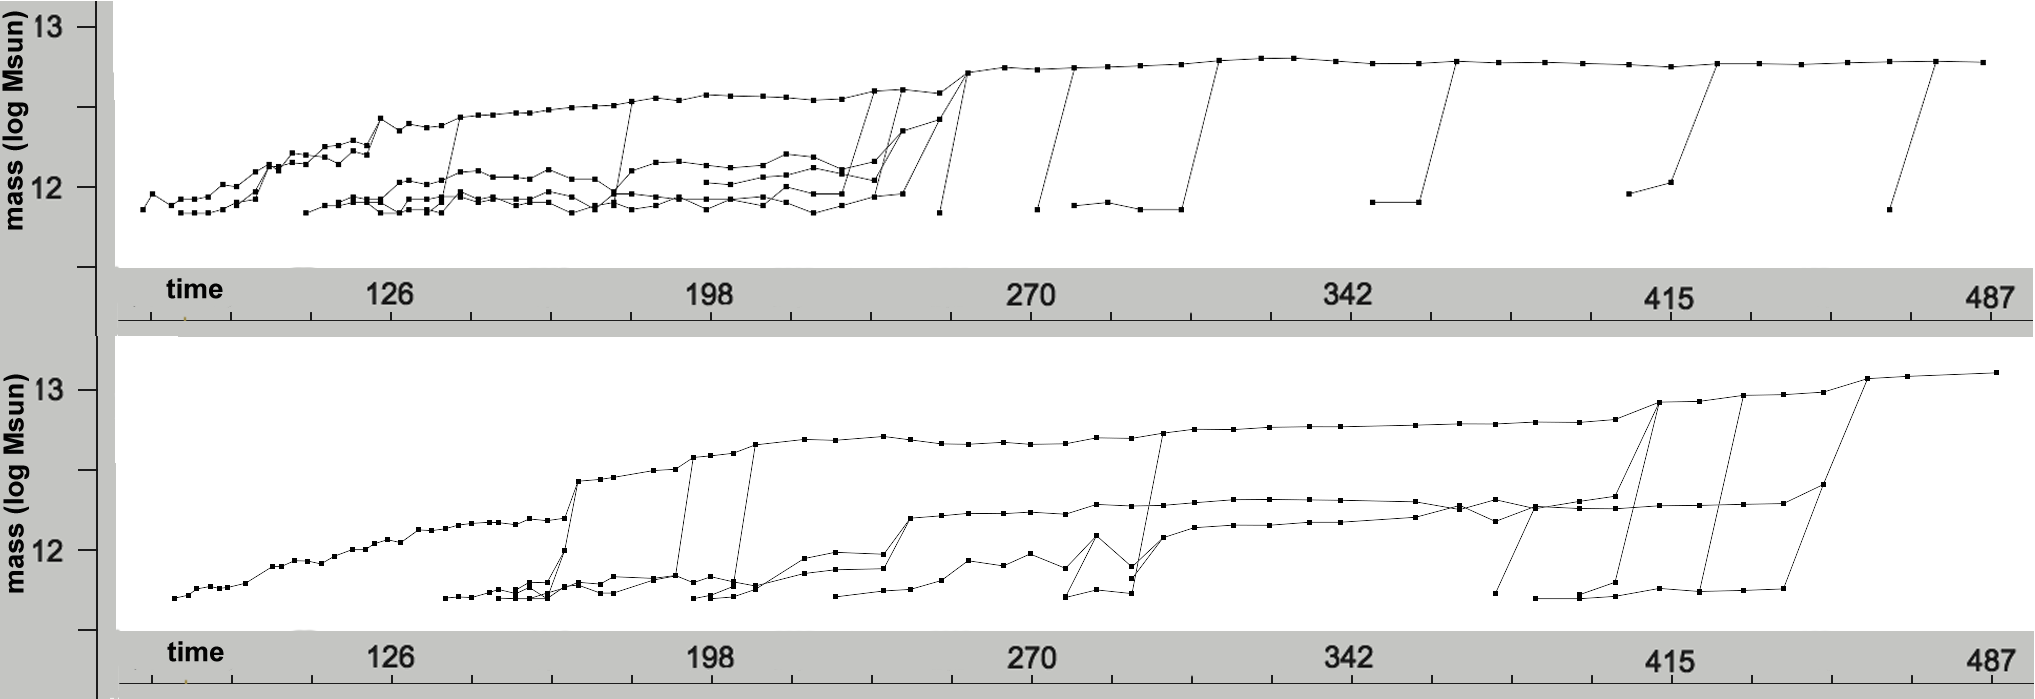
\includegraphics[width=\textwidth]{images/darkmatter/10_v_100_newest.png}
		\caption{Comparison of one merger tree using a 10-particle per halo minimum (top) and a 100-particle per halo minimum (bottom). Because the smaller minimum allows more distinct progenitor halos to be identified early on, the behavior of each tree differs significantly over time.}
		\label{fig:10vs100}
	\end{figure}

From these two images, one can observe how the definition of a halo alters our understanding of the merger tree over time. Though several of the significant merger events are the same in each scheme, the identification of more early progenitor halos using the smaller minimum particle threshold influences the merger tree over time. The higher threshold hides many small halos that may still play a significant role in halo evolution. Observing similarities between these two examples can be used to verify the correctness of the merger tree codes. Moreover, the differences highlighted by this visualization tool can aid scientists in choosing an appropriate balance between the size and resolution of the merger tree data, depending on which halo definition results in merger trees that are more reflective of reality. This comparative visualization makes differences apparent, which may help refine what the correct parameters of a dark matter halo should be, a notion that is still ill-defined~\cite{Knebe:2011}.

	\begin{figure}[t]
		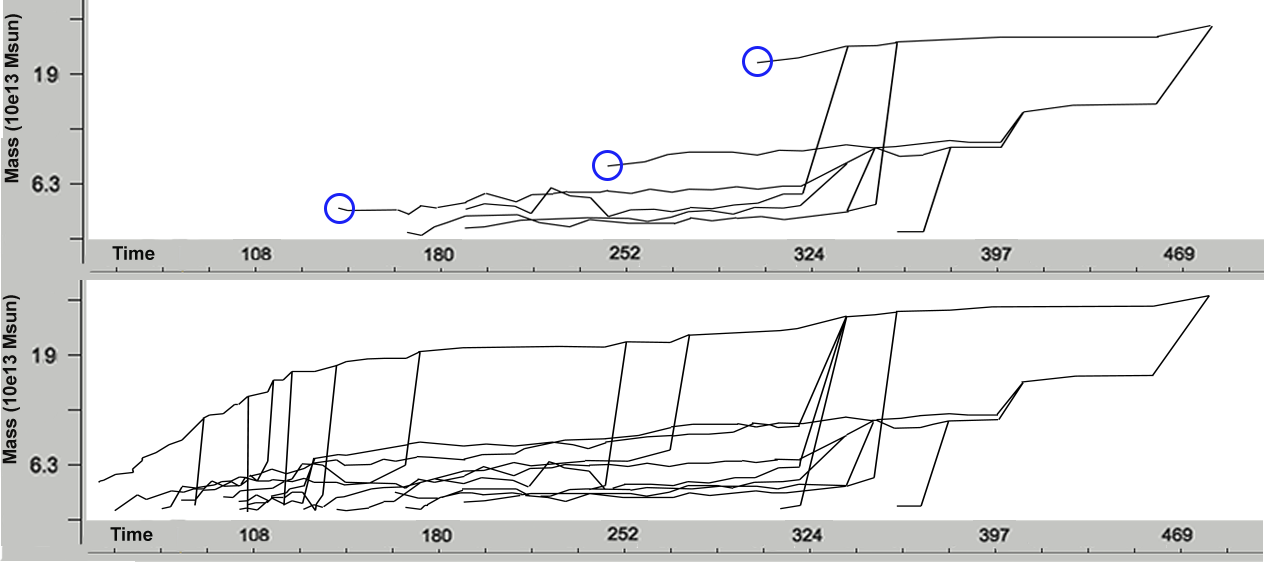
\includegraphics[width=\textwidth]{images/darkmatter/old_vs_new_tree.png}
		\caption{Comparison of two merger trees before (top) and after (bottom) an update to the merger tree finding algorithm. The presence of heavy birth phenomena, circled above in blue, is significantly reduced in the lower tree as very massive halos are now linked to smaller progenitors.}
		\label{fig:oldvsnew}
	\end{figure}

Figure~\ref{fig:oldvsnew} shows another set of merger trees being compared using our system. The top tree shows the presence of many heavy births events. After an update to the merger tree finding algorithm to more carefully account for possible halo splitting, we see significantly fewer heavy births in the lower tree. These are just a few examples of how our visualization tool can provide direct feedback to scientists modifying simulation parameters and algorithms.

\subsection{Performance Results}
The reduced scales of the halo and merger tree data make them easily manageable on a local desktop computer. Furthermore, given the fact the visual clutter will overwhelm users when viewing too many trees at once, only smaller subsets of this data type will be loaded at any given time. As a result, the merger tree and quantitative views are fully interactive with little to no noticeable lag. The particle data is much more massive and requires a distributed framework to render interactively.

The performance and scalability of our renderer was tested on the Cooley visualization cluster at Argonne National Laboratory. Cooley has 126 nodes, connected via a FDR Infiniband interconnect. Each node has 12 CPU cores at 2.4 GHz, 384 GB of RAM, and a NVIDIA Tesla K80. GPU memory is the theoretical limit for the number of particles we can allocate each GPU, but in practice, one would lose interactivity long before running out of memory. When running, we allocate two ranks per node, and assign one rank to each GPU.

\begin{figure}[t]
	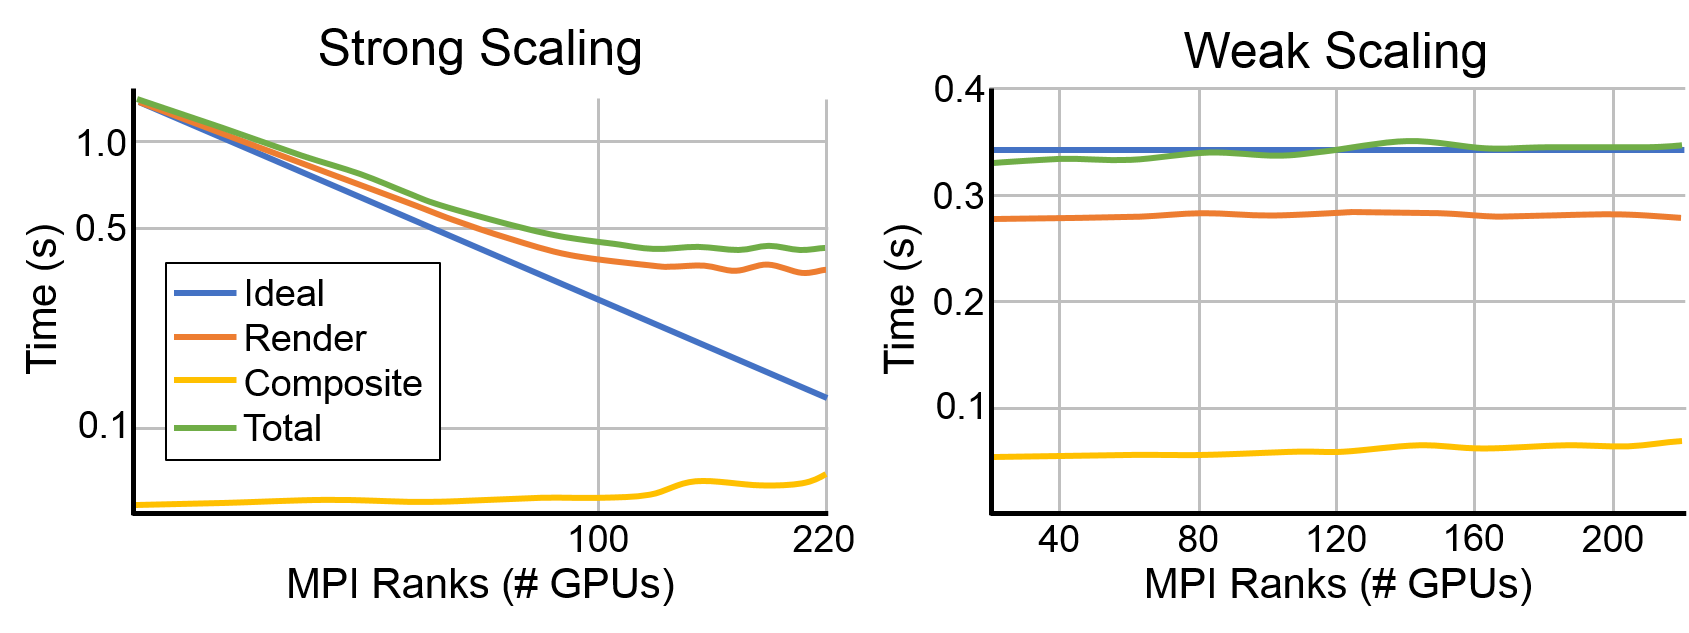
\includegraphics[width=8.5cm]{images/darkmatter/test_scaling2.png}
	\caption{The log/log plot of strong scaling results for our system (left) shows a decrease in performance at large numbers of nodes, indicating an overhead cost of the renderer. Weak scaling (right) shows nearly ideal total rendering time across all machine sizes.}
	\label{fig:scaling}
\end{figure}

We conducted strong and weak scaling studies to assess our system (figure~\ref{fig:scaling}). The ideal time is defined as $t_0 / N$ for strong scaling, and $avg(t_0, t_N)$ for weak scaling, where $t_i$ is the total time for the machine size $i$, and $N$ is the maximum machine size used in our study (220 GPUs). Each measurement is the average of 42 views evenly distributed around the outside of the data volume in order to make the time measurements view-independent. The full data was used for every machine size in the strong scaling study. The number of particles per node for the weak scaling study, 5368619, was kept constant by partitioning the data as normal, then selecting a random subset of the particles from the partition assigned to each node.

Our strong scaling results show good scaling for this dataset up until 80 nodes, after which our times diverge from ideal scaling. We believe this is due to a constant overhead cost in our renderer, and that there is room for optimizations to reduce this overhead. The weak scaling results, where the total rendering time is close to the ideal scaling time across all machine sizes, reflect the scalability of our system.

\section{Discussion}
We designed our tool so that it has the flexibility to visualize cosmological data from sources other than HACC. Since data from many other cosmology simulations are similarly split into the particle, halo, and merger tree representations, our visualization tool can not only be used to compare results between different runs of a simulation, but also between different types of simulations. This comparison can be useful when comparing different computational models of universe formation, such as comparing an N-body gravitational simulation with one that includes hydrodynamic effects.

Our ability to interactively explore the large datasets produced by simulations in the HACC framework demonstrates our tool's scalability. The remote particle renderer allows for the visualization of even larger datasets: additional particles can be included with very little increase in overhead by incorporating additional computing nodes. The highly parallel nature of distributed particle rendering ensures that communication costs between nodes can be kept small.

Future simulations, with finer mass resolution and more particles, will produce too many merger trees to be handled efficiently at a local level. Therefore, we plan to implement all three visualization views in a remote and parallelized setting. In this scheme, all data produced by the simulation can remain in place while analyzed remotely from a desktop computer. This will reduce the I/O costs associated with data transfer between different locations. 
Due to the highly interconnected halo, progenitor, and descendant data, implementing the merger tree view in a distributed manner can result in large communication costs between computing nodes. In order to maintain interactive speeds, some form of node-level data redundancy may need to be implemented for this view.

Interactive analysis of cosmological simulation data is vitally important to preparing for upcoming large-scale astronomical surveys~\cite{skysurvey}. It is important to hone an accurate model of structure formation in the universe, which astronomers believe is dictated by the evolution of dark matter halos. Because these halos cannot be directly observed, a solid theoretical understanding, guided by simulations, is necessary to link theory with observational data. If correct, these simulations should produce results, such as the mass and brightness distributions of galaxies, that match those observed in surveys. Any differences between the two may point to a further refinement of simulation algorithms.

Flow visualization is another broad area that can benefit from such a visualization tool. The large particle-based data in Lagrangian flow representations can be visualized using our parallel particle renderer. Any accompanying Eulerian features and regions of interest that are identified and tracked throughout the simulation can also be displayed using our merger tree visualization. Moreover, linking these views can enhance the exploration of particle and feature correspondence and lead to finer understanding of underlying processes.

\section{Conclusion and Future Work}

We have created a system for interactive analysis of large cosmological simulation data. By linking views of multiple simulation data types, we offer an opportunity to gain new intuition for simulation code behavior and for features of interest in the universe.

Due to the very large, and increasing, scales of simulation and observational data, future work must focus on improved capability for interacting with large data sets. In particular, we hope to work with a larger version of the data set addressed in this paper, and include capability for smooth animation over several time steps. We also aim to provide improved capacity for viewing quantitative information from throughout a halo's history, which is costlier to look up than data from the present time step.

The application of visual diagnostics to cosmological datasets has vast potential for future work. In addition to refining merger tree models for the evolution of dark matter halos, scientists also seek to characterize specific properties of halos, such as their alignments and centers of mass \cite{Behroozi:2013}. The calculation of minimum potential needed to find halo centers is expensive, and the result is likely to change drastically depending on the properties of the halo-finding algorithm. Visual analysis, with a complementary 3D view and quantitative information, would help troubleshoot the results of center-finding codes. There is also great interest in exploring related topics such as multi-streaming and structure formation events \cite{Popov:2011}, and using semi-analytic models to superimpose galaxy information onto dark matter simulation data, which may then be compared directly to observations. With help from visual diagnostics, the trend towards accuracy in cosmological simulation analysis will enhance scientists' abilities to learn from the largest, most ambitious observational sky surveys.
\chapter{Cluster-Based Visualization Design for Merger Tree Data}

%NOTE: convince the audience that this is a very common problem that limits the types of things that we can use clustering for!

% can talk about the scatter plot experiments, and the progenitor-drawing experiments, to convince that we've explored a big chunk of the possible design space

% big simulations are common; visualization can help analyze them, but it's hard at increasing scales.
Across domains such as astrophysics, atmospheric science, particle physics, and fluid dynamics, scientists are using growing computing power to create increasingly high-resolution simulations~\cite{hacc},~\cite{Steed:2013:BDV:2538033.2538071}. Simulated models of physical systems allow scientists to perform a range of important tasks: explore how external variables affect physical systems, compare simulated and observed data, and project outcomes. Visual analysis can be an important tool for understanding such simulations, but increasing data size and dimensionality challenge traditional visualization approaches with clutter, obstruction, and overburdened visual channels~\cite{taxonomy_clutter_reduction}. %^ this paper notes that the problem is worse for unstructured exploration, as opposed to investigating something in particular

% clustering is one approach. here are a bunch of examples that establish the scope.

%visualizations that use clustering.
A common solution is to aggregate simulation data, then visualize information about the resulting groups. Clustering is applicable to a wide range of data---it primarily requires defining the ``similarity'' between any two data points---and often, clusters have a natural, scientifically significant meaning. The process can help categorize physical phenomena and characterize overall trends. Visualization researchers have applied clustering to a wide range of applications (see Section~\ref{relatedwork}). Outliers can be exposed in the clustering process; these outliers may indicate interesting scientific phenomena or problematic simulation code. Approaches such as hierarchical clustering allow for intuitive multi-resolution exploration so that scientists can understand trends and outliers at many levels of detail. 

% but, clustering abstracts the data, partly because of the black box, and also we're a bit in the dark because the above examples don't really validate whether the clustered results are helpful.
However, clustering abstracts the underlying data into information about groups of the data. This abstraction is a loss of information about outliers, noise, subtle differences between time series, and data-processing steps. Growing data sizes magnify the threats from abstraction, because more data are being represented per visual element.  The ``black box''---or unseen inner workings---of a clustering algorithm is another significant source of the threat from abstraction. 

%There are few visualization efforts to show information to the user about how the clusters were generated. (TRUE?/CITE EXAMPLES)
%The visualizations of clustered data listed above do not depict the process of deriving clusters from the data. [this is hard to depict - CITE - ?]
% IMPORTANT: would be good to show through the examples that clustering isn't necessarily the only solution here, but abstraction in some sense always has to happen

% at least in those examples, though, there are often expectations for clusters/natural groupings. some data, like ___ or merger trees (see section __), don't have natural groupings but face a big data/vis problem. 
In some cases (see Section~\ref{relatedwork}), expectations for the groupings can help users make sense of a clustered visualization despite the abstraction and black box, which provides some validation. However, there may be only vague expectations for trends and groupings within simulation data. This is the case for simulated dark matter merger trees (see Section~\ref{background}). We explore a clustering visualization approach for merger trees from N-body simulations. We propose that, for a clustered, abstracted representation to enable useful visual analysis of these data, we should provide flexible clustering options, linked multidimensional views, and information about the black box. 

%In our preliminary survey, this limited scientists when interpreting visualizations of clustered merger tree data. % be more explicit about 'confused' 

% here, we see if we can address this problem (for one case) by 1) providing strongly multidimensional and controllable clustering vis and 2) showing the black box 

In this work, we develop the following to enable more meaningful representation and exploration of merger tree data:  

\begin{itemize}
\item{Problem characterization and abstraction~\cite{trenches_stacks} for analyzing dark matter merger trees.}
\item{An extension of the contour boxplot~\cite{contour_boxplot} for groups of multivariate time series, which enables visualizing groups of unconventional data structures like trees.}
\item{A flexible clustering approach to support free-form exploration and user-defined centroids.}
\item{A visualization approach for understanding the pairing process in a clustering algorithm.}
% FUTURE: \item{A reflection on existing design guidelines in the context of this application's particular challenges.}
\end{itemize}

%%%%% BACKGROUND %%%%%

% sum up why merger trees are a particularly hard domain, and sell that addressing the problems for it is a good pursuit.

\section{Analyzing Dark Matter Merger Trees}
\label{background}

% what are merger trees and why should we care?
Scientists use simulation frameworks such as Illustris~\cite{illustris_info} and HACC~\cite{hacc} to study how dark matter forms its structure in the universe. The simplest approach is an N-body simulation: initially, dark matter ``particles'' are distributed throughout a volume. The gravitational attraction among particles creates dark matter ``halos'' that merge into one another to become increasingly large halos. Each halo present in the final timestep can be characterized by its history: which halos merged together to form this particular dark matter clump, and when? The plots of these halo histories, actively studied in cosmology research, are called ``merger trees'' (see Figure~\ref{diagram}).

One reason to study halos and merger trees is that galaxies, which contain the majority of their mass in dark matter, form within halos. Merger trees may help explain the connection among dark matter halos, their environments, and how galaxies form within them. For an in-depth discussion of dark matter halos, merger trees, and galaxy formation, see~\cite{lacey1992}.

% what is the workflow/scientific process for analyzing merger trees?
	% how do they find outliers?  
    % for good analysis, one needs to be able to see all the data, identify trends & different types of outliers
Through literature review and a survey of several researchers studying merger trees in N-body simulations, we identified tasks and guiding questions for analyzing dark matter merger trees~\cite{hacc},~\cite{masshistory},~\cite{lacey1992}. We also proposed the idea of clustering trees into groups and solicited questions about that approach.
\begin{itemize}
\item{Do halo properties, e.g., \textit{concentration} or \textit{formation time}, correlate with characteristics of their merger trees?} %‘in what sense is concentration a classifier of histories?’%}
\item{Can we identify anomalies such as missed progenitors or heavy births (i.e., instances where the sum of progenitor masses does not explain a halo's mass, or where a new halo is identified by a halo finding algorithm that was not present in previous timesteps)?}
\item{When, and why, do anomalies in the simulation appear?} %note for later: this needs a system like our previous one to be investigated, but that system needs a complement (This system) to facilitate actually finding the outlier trees.
\item{How many outlier and non-outlier merger trees are there?}
\item{What is the measure of similarity between trees for forming the clusters?}
\end{itemize}

% ... clustering can potentially answer these questions because ____.
Done correctly, clustering may be a scientifically meaningful approach to visualizing merger trees that could address the above questions. Most trees likely follow only a few different types of mass histories throughout their lifetimes~\cite{masshistory}, meaning they can naturally be grouped into clusters that describe these patterns. Outliers, which might represent a unique physical phenomenon or a code bug, can be placed alone or in smaller clusters if the similarity metric singles them out (see Section~\ref{clustering}). A cluster-based visualization for merger trees may be successful, then, if the similarity metric identifies meaningful, non-arbitrary groupings and outliers, and if the properties of the resulting clusters are intuitive to viewers.

%mention somewhere?, that in the preliminary survey, they didn't really know how to answer 'do these clusters meet your expectations'

%establish why we need vis (finding patterns and outliers can be enabled by visualization. 
	% some things (that we're looking for) can be identified analytically but we also don't know what we're looking for
%(galaxy formation is poorly understood; CITE)
    
\section{Related Work}
\label{relatedwork}
One motivation for this study is that existing tools to study ensembles of merger trees are quite limited. Simulations can yield millions of merger trees. Researchers have most often visualized merger trees by rendering each node and edge, such as in~\cite{scivis15},~\cite{Shan:2014} (Figure~\ref{node_edge}). This approach cannot accommodate all output from a simulation. Rendering all merger trees at once prevents scientists from discerning global patterns or individual discrepancies~\cite{ellis2007},~\cite{elmqvist2010}; occlusion from over-plotting particularly affects the many low-mass halos. 

\begin{figure}[h!]
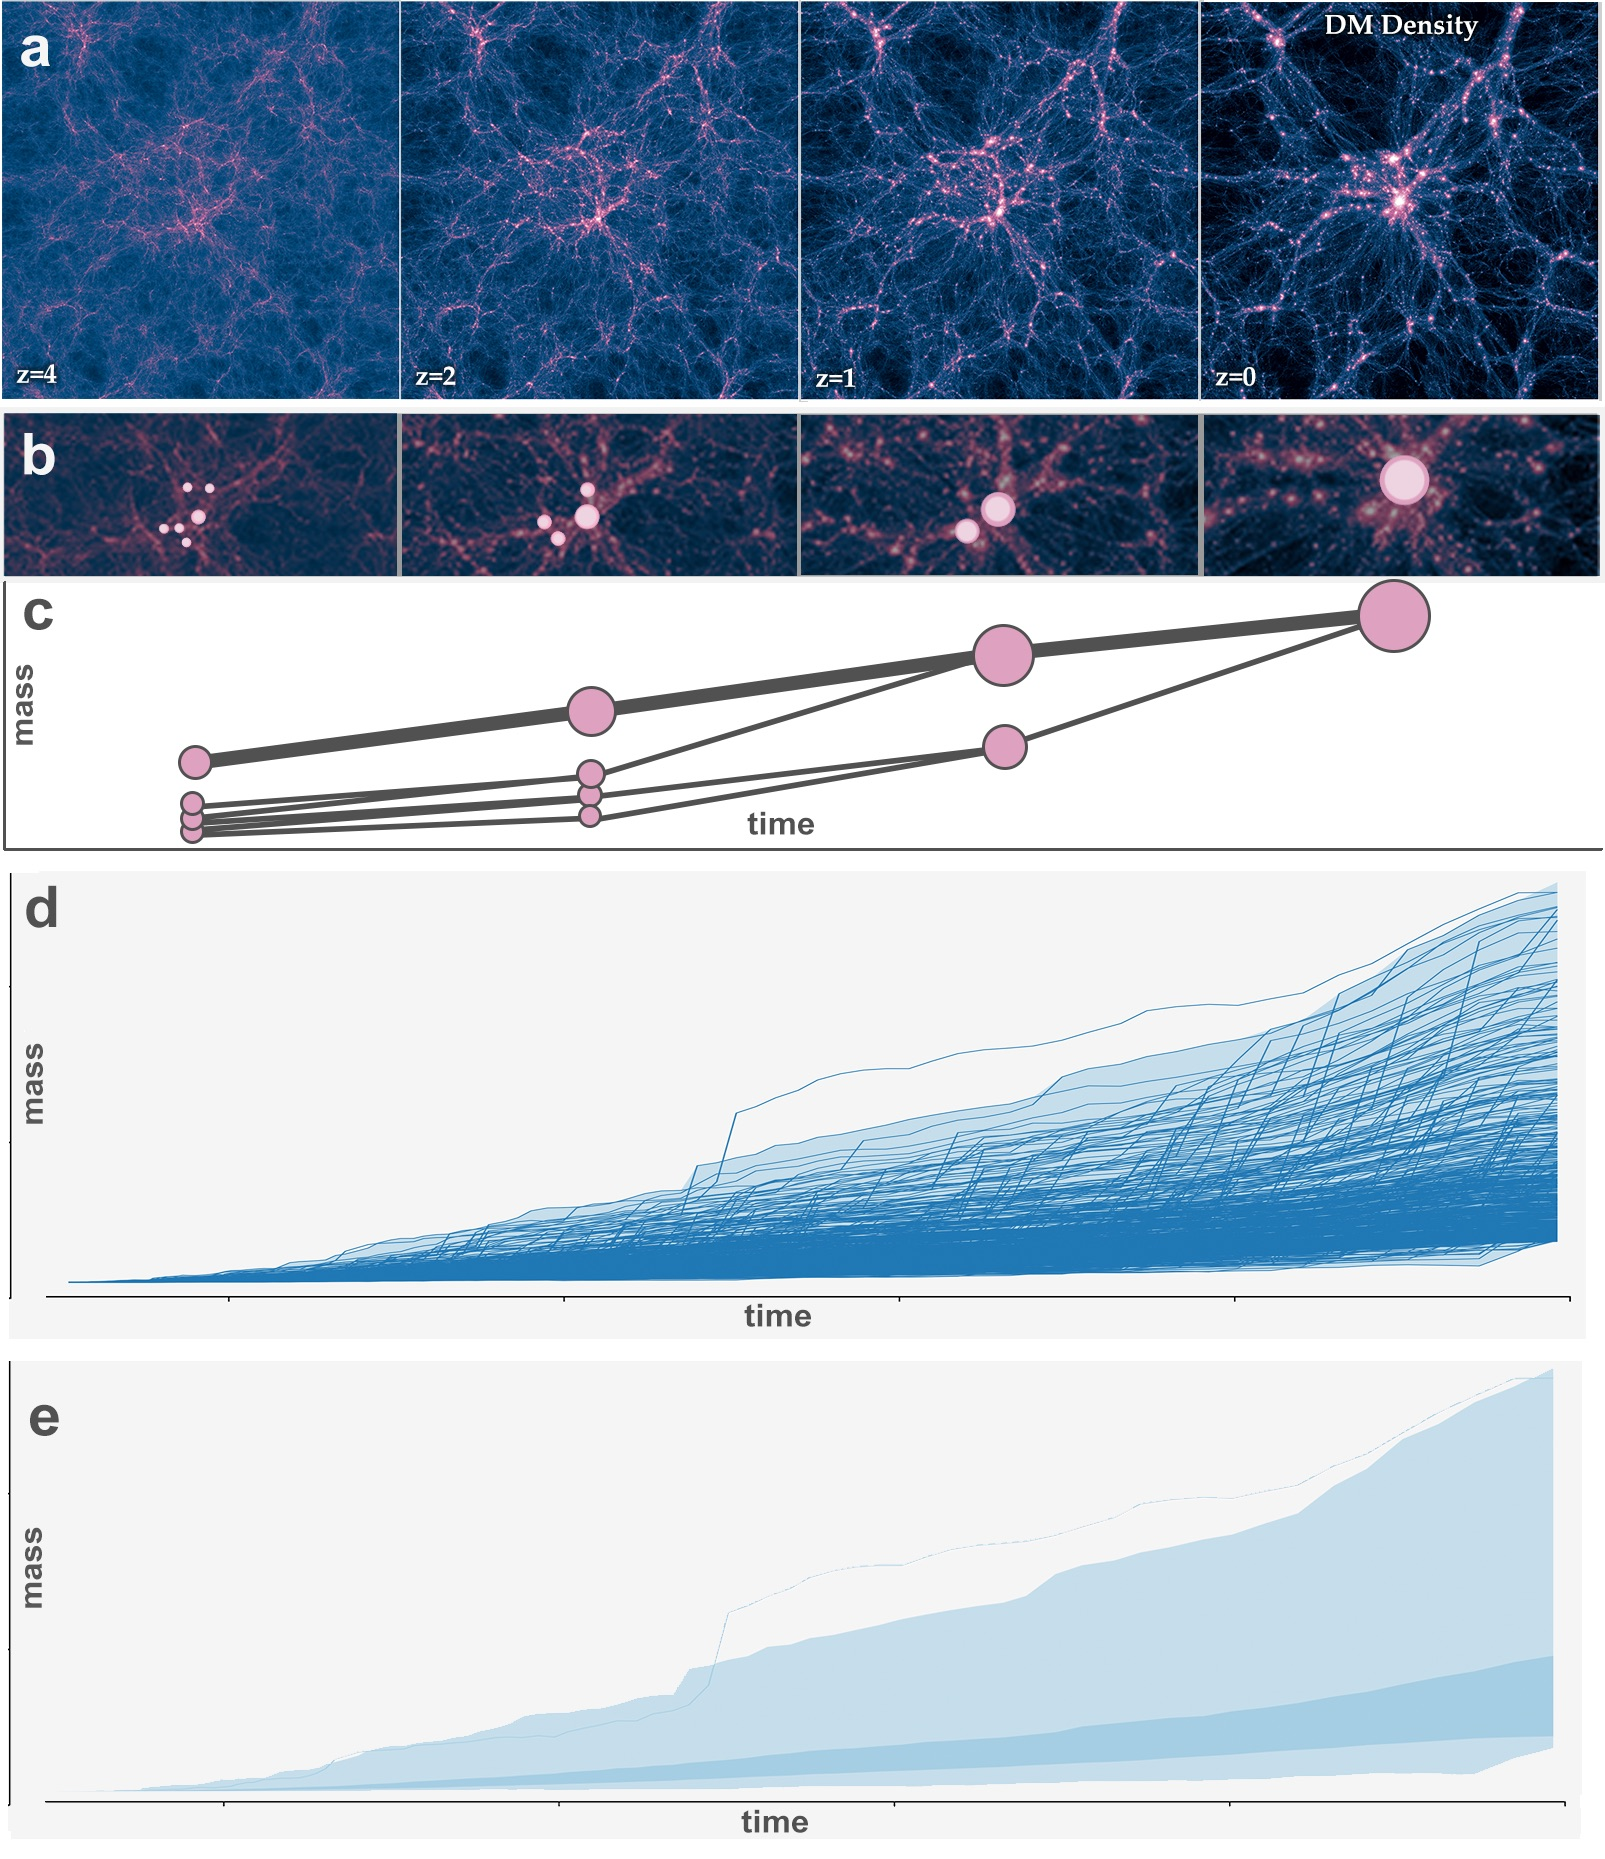
\includegraphics[width=\textwidth]{images/clusters/particles_to_tree_cluster.jpg}
\caption{The process of abstracting dark matter simulation data (a) into clusters of merger trees (e). For each timestep of the simulation, dark matter halos are identified using a halo finding algorithm (b). Here, we show four timesteps of the Illustris simulation (a) (Image credit: Illustris Collaboration). In (b), we highlight the progenitor halos for the single halo in the final timestep on the far right. A simple merger tree (c) shows how halos merge together in each timestep. The ``main branch'' is highlighted. In (d), we show all main branches, over all timesteps, for one mass bin. We represent clustered main branches by their range of values, with the middle $50\%$ highlighted and an outlier rendered separately (e).}
\label{diagram}
\end{figure}

\begin{figure}[h!]
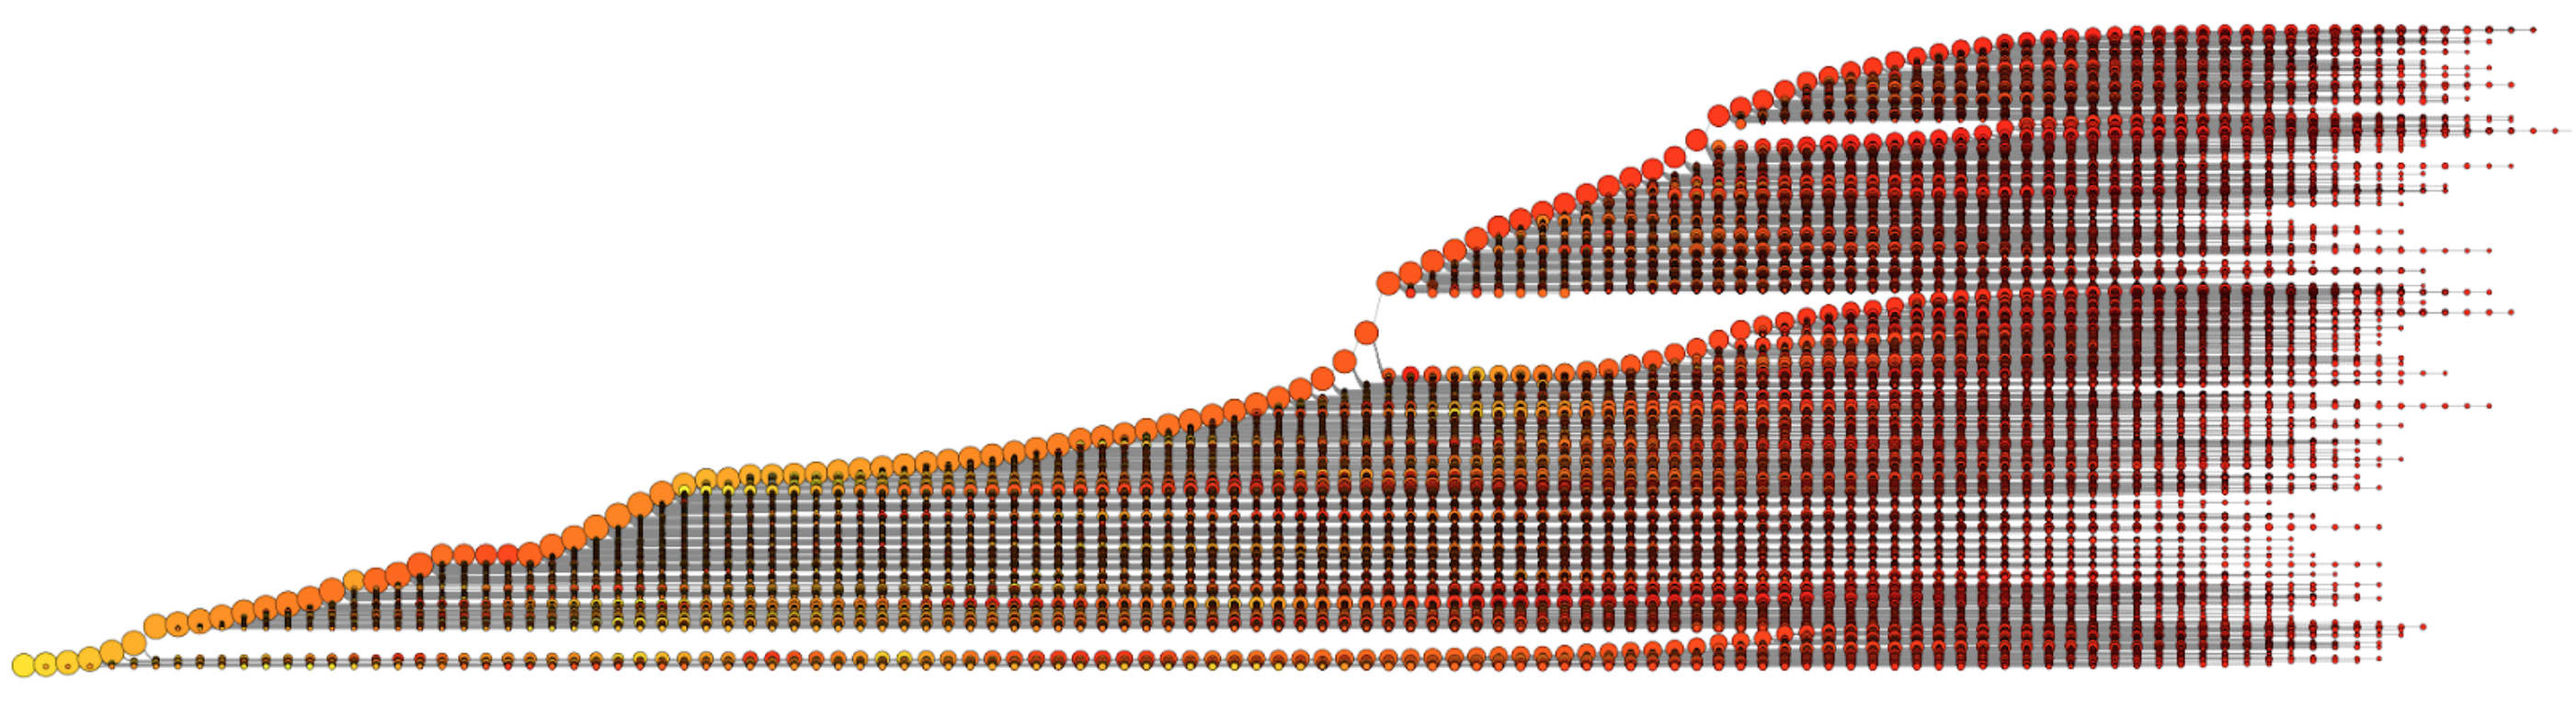
\includegraphics[width=\textwidth]{images/clusters/illustris_tool}
\caption{A snapshot from the Illustris Merger Tree Tool (credit: Illustris Collaboration). The halo masses are mapped to the circles' sizes, and velocity is mapped to color. This approach can show complex progenitor behavior for a single merger tree.}
\label{node_edge}
\end{figure}

Zooming and panning cannot provide clarity, because viewing segments of merger trees very close-up removes context and time-varying trends. %what analysis goes with this? why is it useful sometimes but why is it hard? T
There are also 3D visualization approaches showing the spatial position of each halo throughout the merging history, such as in~\cite{7429496}. %later -- and FIND THIS CITATION. 

% why don't we have expectations for the trends? (cite survey of scientists that we did.)

%clustering applied to scientific data in general.
In general, clustering has been used to help visualize a variety of scientific data. The authors of~\cite{k-means--} create a version of \textit{k}-means with enhanced outlier detection and test it on a set of hurricane trajectories. The outliers identified are not compared to the non-outliers and do not seem to have clear reasons for being outliers.

%~~~~
The authors of~\cite{wei2012} propose a fast, scalable clustering technique for multi-length data from combustion simulations that allows the clusters to be subject to users’ specifications. However, this approach for visualizing particle paths lacks scalability: it uses sight-based outlier rejection, which requires that only a small number of particle trajectories are rendered at once. It is unclear how to make sense of a larger dataset or a larger group of clusters. Another approach, explored in~\cite{hier_parallel}, uses a parallel coordinates representation with gradiated bands to visualize aggregated data. Parallel coordinates can also be used in a focus + context visualization in a way that preserves outliers~\cite{outlier_parallel_coords}. The authors of~\cite{group_dynamics} create a group feature tracking framework for scientific data which is shown to be effective on turbulent flow data; this work does not focus on scientific usefulness or on specific use cases. 

A unique approach in~\cite{weather_ensembles} aggregates ensembles of weather forecasts, visualizing when and how various forecasts diverge. In~\cite{ocean_models}, the authors develop a specialized approach for aggregating ocean model data based on clustering ensembles, allowing scientists to compare simulation output with observations. The work in~\cite{relevant_parts} establishes an interactive visualization method for defining relevant parts of trajectories in 3D space and interactively refining the clustering. Finally, the clustergram~\cite{clustergram} is a scalable clustering visualization method that can show how items are added to clusters; this could be useful for opening up the “black box” of clustering to end users.

%~~~~~~

\begin{figure*}[h]
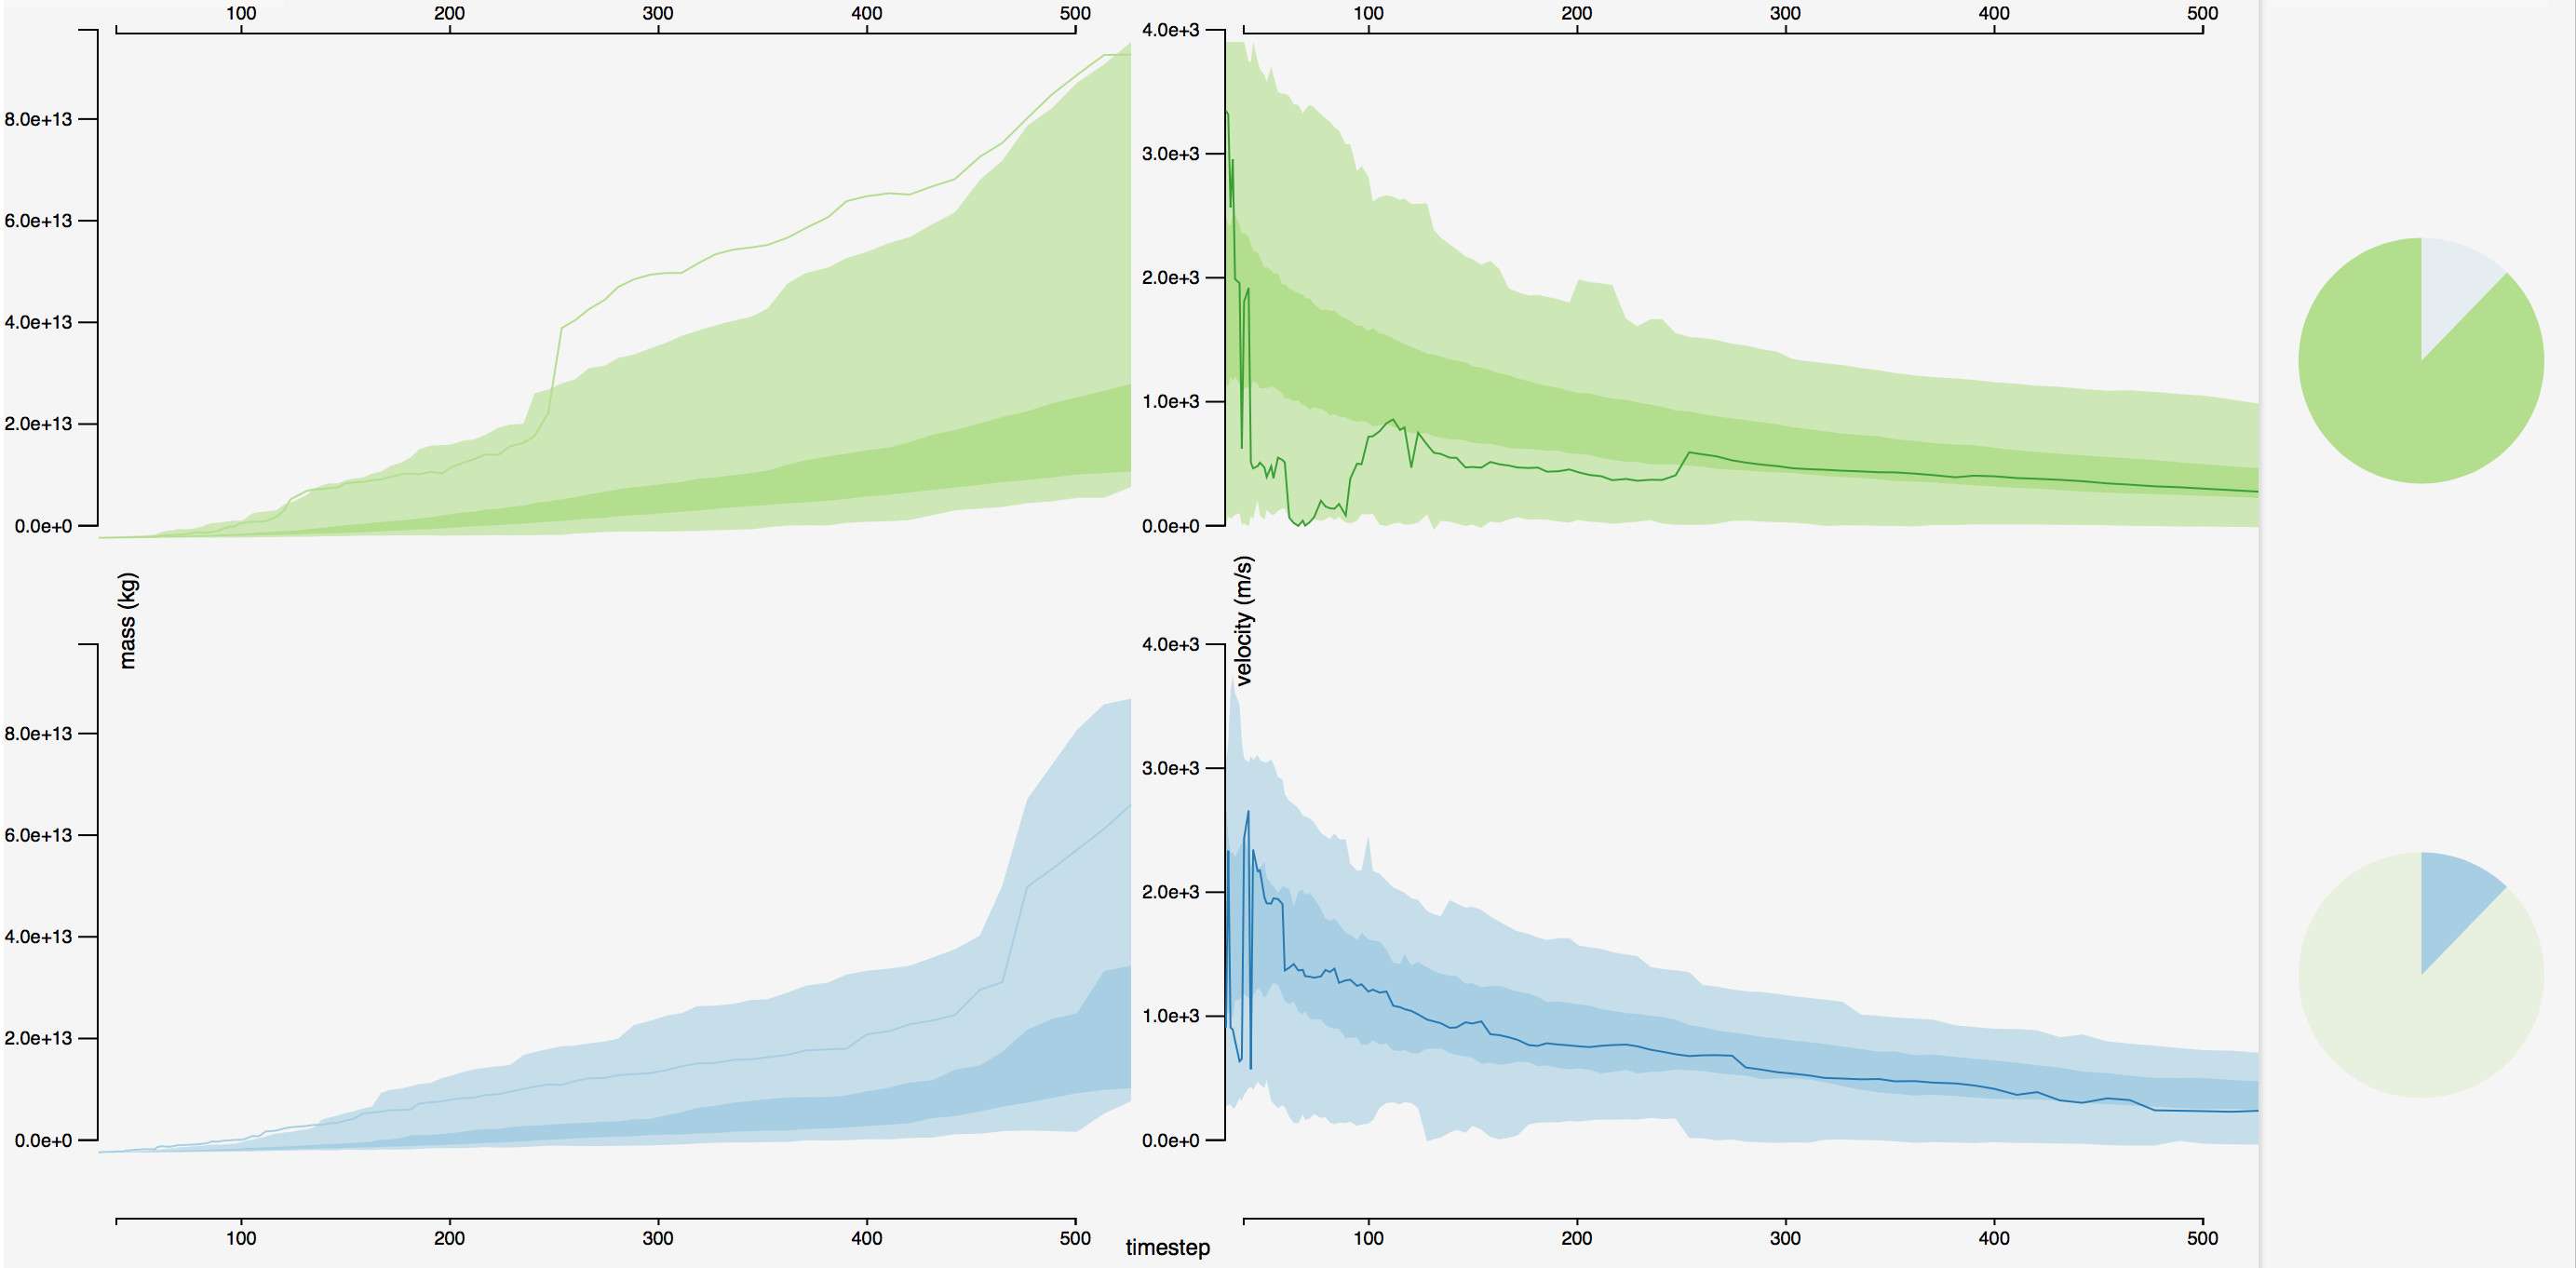
\includegraphics[width=\textwidth]{images/clusters/n2_mass_velocity_outliers}
\caption{Mass (left) and velocity (right) for a single mass bin with $n_{\mathrm{clusters}}=2$. Outliers are highlighted in each view (the outlier is the same tree for the mass view and the velocity view). While the blue outlier seems similar to the rest of its cluster, the green outlier merits further exploration. It has an unusually low mass for the first half of the simulation, then experiences a large mass increase and a sudden velocity shift around $t=250$.}
\label{vel_example}
\end{figure*}

%%%%% METHODS %%%%%

\section{Design Decisions}
%* identify threats (abstraction, distrust) for each choice

%* couch this in terms of existing design guidelines, as mentioned by pvast reviewer

We use data from a run of HACC~\cite{hacc} that yielded about four million merger trees, each including thousands of data points with position, velocity and mass. Based on our preliminary survey, we choose to group the merger trees by binning their root masses; this is a common approach~\cite{masshistory},~\cite{assemblyhistory}.
%(can leave out:)
%(explain?)

\begin{figure}[h]
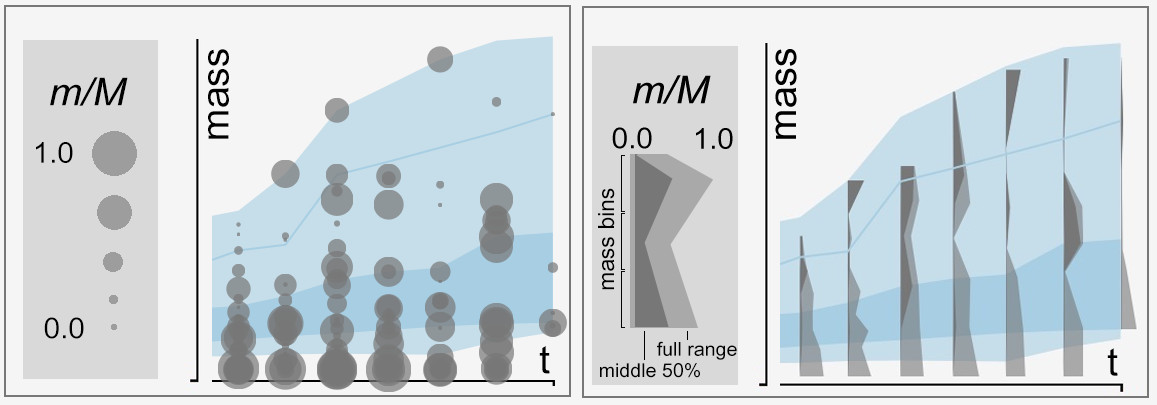
\includegraphics[width=\textwidth]{images/clusters/merger_abstraction_diagram}
\caption{How we abstract merger data in our approach. On the left, a circle for each merger represents the merger ratio $m/M$, i.e., the ratio of progenitors to the main branch halo being merged into. Low-mass halos clutter this representation. On the right, we use a modified violin plot to represent the range of merger ratios (horizontal axis) for each mass bin (vertical axis) at each timestep.}
\label{merger_abstraction}
\end{figure}

\subsection{Defining Clusters}
\label{clustering}
%better DTW example image, with real data (i.e. in our view)

%overall: mass is a baseline because it's the most intuitive/common thing to go with
% Many data clustering algorithms were designed for numerical data~\cite{clusteringbook}, in contrast to continuous data common in scientific simulation outputs such as mass and velocity.  %therefore, ...?
% ^^ PUT THIS IN FULL VERSION. /quals.
% there's a lot of info for clustering to abstract away
For visual analysis in general, data science approaches like clustering are best for ``crisply defined tasks''~\cite{trenches_stacks}, rather than the broad exploratory questions considered in this study.
%therefore?
Additional challenges include that merger trees have varying lengths in time, and that mass and velocity values can differ by nearly an order of magnitude. 
% and of course, no ‘natural’ clusters or subsetting; only a few percent might be interesting; 

% dist metric: want the clustering to be based on scientifically/physically significant similarities/differences
Clustering data requires a “distance metric” that measures the relative similarity of data points, i.e., the similarity of two merger trees. In our case, this metric depends on a set of features representing each merger tree. To choose these, we can use \textit{feature extraction} or \textit{feature selection}. Feature extraction includes techniques like Principal Component Analysis~\cite{clusteringbook}, which warp data into a lower-dimensional representation by combining parameters. Feature selection, instead, uses a set of existing attributes---in our case, mass, velocity, number of mergers, etc.---to characterize data.

% NOTE: here, doing feature selection, we explore the design space ~of the existing parameters~. this gets us pretty far because we can see that mergers are really important while velocity (and spatial position) are not that telling. if we use feature extraction, we can explore a much larger space of options, like combined effects of two variables.

Feature selection has an intuitive interpretation, while feature extraction yields more complex features that may have greater predictive power but a more arbitrary meaning~\cite{clusteringbook}. Both approaches can contribute to abstraction by masking the data's underlying properties. To reduce abstraction, we use the most common approach in cosmology research: feature selection using the main branch mass representation~\cite{masshistory},~\cite{assemblyhistory}. This decision eliminates clutter by removing low-mass halos, which have relatively small effects on their merger trees and are often omitted from analysis.

We choose Dynamic Time Warping (DTW)~\cite{clusteringbook} to calculate the distance between each pair of main branches. DTW accommodates time series of different lengths and with inconsistent sampling frequencies, such as merger trees. It calculates how much one time series would have to warp in order to match another time series. A pair of merger trees can be ranked as similar if they share main branch features shifted by some time phase. 

%%FIGURE
\begin{figure*}[h]
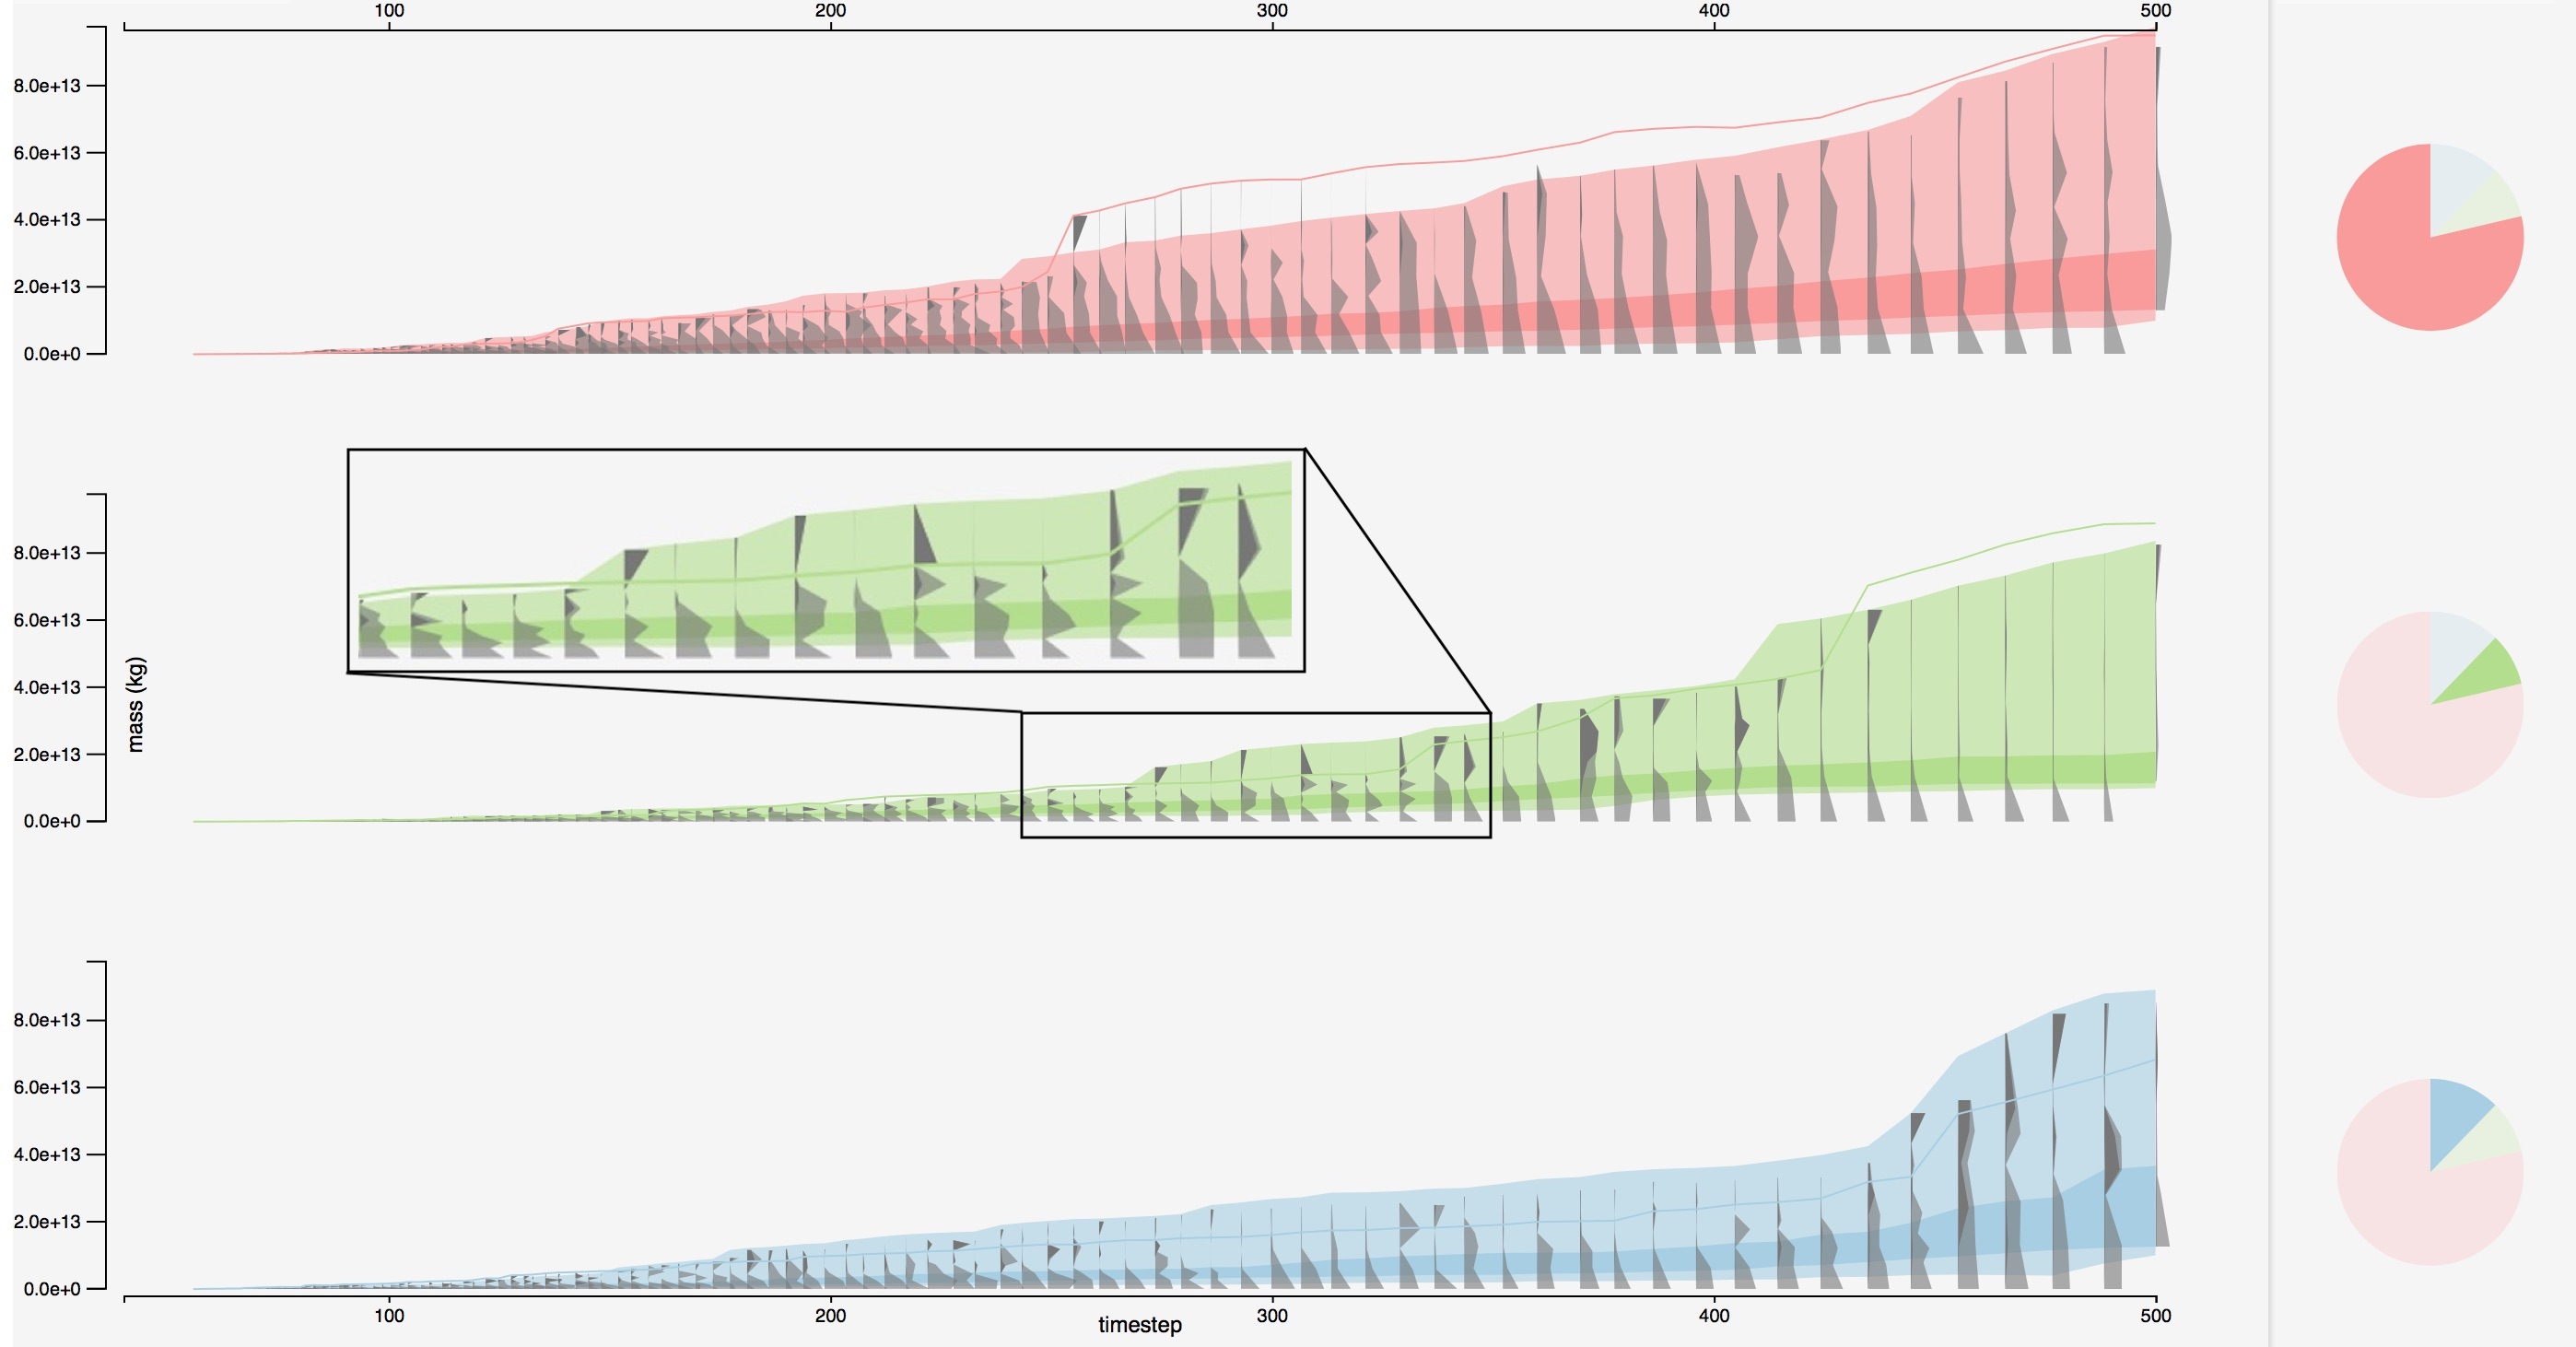
\includegraphics[width=\textwidth]{images/clusters/n3_d0_with_mergers}
\caption{Merger trees for one mass bin ($10^{13}\mathrm{kg} < M < 10^{14}\mathrm{kg}$), divided into three clusters based on DTW similarity for main branch mass. The colored shapes show the distribution of main branch masses over time, while the gray shapes show distinct merger activity for each cluster (see Figure~\ref{merger_abstraction}). One outlier per cluster is rendered with an individual line. At right, pie charts show the relative proportion of trees in each cluster.}
\label{three_clusters_with_mergers}
\end{figure*}

%linkage: unclear; difficult to visualize; we offer the choice because \shrug and this doesn't bias them too much at least hopefully
We also need to define the similarity between two groups of main branches. This option is known as ``linkage.'' Three common linkages are \textit{single}, \textit{complete}, and \textit{average}~\cite{clusteringbook}. Linkage significantly affects clustering results. Single linkage has the tendency to form ``long chains,'' adding most members to one cluster while leaving outliers unpaired. These clusters might contain quite disparate main branches, but the outliers left exposed should be even more disparate. Complete linkage tends to form clusters with more consistent characteristics and sizes [42], perhaps yielding better summaries of the data set.
In this step, we may be trying to group data that do not necessarily fit neatly into categories. However, we find that average or complete linkage is useful for characterizing merger trees, while single linkage better distinguishes outliers (see video).

At each step in the algorithm, the two merger trees or groups with the smallest distance are grouped; this creates a hierarchy of clusters. We can query the hierarchy at any level to return the desired number of merger tree groups. These DTW-generated groupings provide the default for our visualization. However, to provide more flexibility, we allow users to pick a tree as a centroid around which to re-cluster the data.  For now, we only implement $n=2$ as a proof of concept. Therefore, for each new centroid, we only have to check the distance matrix once to find the maximally distant tree, define that tree as the other centroid, and then define clusters based on the nearest centroid. These results can address our scientific goals: scientists are interested in how many outliers of each type there may be, and how much they diverge from other trees.
This approach can be further improved, such as narrowing the neighborhood around the target centroid in order to get more precise groupings.
%(see supplemental video!)

%%%%% VISUAL ENCODING %%%%%
%...these are the choices, and this is how they abstract the data.

\subsection{Visual Encoding}
%challenge: we're visualizing a pretty abstracted set of data; 
	% inconsistent number of data points per timestep per series, so hard to depict distributions of distributions
    
% 0th: overall guidelines we'll try to follow:
First, we establish design guidelines: the authors of~\cite{Albers:2014:TEA:2556288.2557200} suggest that color is best for ``summary comparisons,'' especially when the aggregation is not explicit, and that position is best for ``point comparisons,'' i.e., comparing individual data points. We use color to indicate categories, designating a color family for each cluster. We use position for comparison among clusters, providing a common baseline of a quantity vs. time, as suggested in~\cite{graphical_perception}.

% SAY THAT WE SHOW DTW PAIRS IN THE VIDEO.

\subsubsection{Clusters and Merger Trees}
%first, how to make the visual aggregates:
%contour boxplot to show distributions of paths; 
One framework for visualizing aggregated data~\cite{elmqvist2010} suggests creating \textit{visual data items,} i.e., single merger trees, and \textit{visual aggregates,} i.e., clusters. These aggregates should describe the data points within that cluster, such as how many items exist in a cluster, the average and spread of their values, and the timing of significant events. Existing visualizations of groups of paths, such as~\cite{contour_boxplot}, often show distributions of univariate quantities over time. We extend this to include other features like halo velocities, timing and sizes of mergers, and number of progenitors. We separate the dimensions and provide multiple contour boxplots at once for univariate features like velocity (see Figure~\ref{vel_example}). For some features, there are multiple measurements per item per timestep (mergers, number of progenitors); this requires visualizing a distribution of distributions (see Figures~\ref{merger_abstraction},~\ref{three_clusters_with_mergers}).

%(vis research says to not use dual axes for this). 
%we do use the same axes when the properties can be mapped to the same axes, though. otehrwise, separate plots (or indexing?).
% we don't implement indexing here, but can mention as a possibility.

%Contour boxplots fulfill the above guidelines by indicating the middle $50\%$ of each cluster as well as outliers. In (CITE), only (?) outliers are shown, but this is arbitrary and may hide other important outliers. Therefore, we offer the option to select a particular merger tree, then re-cluster using that tree as a centroid (see video). Once we calculate the distance matrix, this can be done quickly. %how to find other centroids?
% talk about outlier definition -- mention more sophisticated ways of doing it with dtw
%how do we implement clustering around a reference centroid? DO THIS.

%we also need visual items
%(don't want to entirely eliminate this information; want it as a reference)
As context for the abstracted clusters, we provide the option to overlay time series within the cluster (these are the ``visual items''). We include the option to view a random subset of the merger trees in a cluster, or merger trees that represent ``edge cases.'' Describing clusters using randomly selected members should provide a representative description, and edge cases may be interesting outliers.

\subsubsection{Clustering Process}
%here are the challenges/pitfalls in our vis approach of above

%Each choice made so far potentially introduces another bias or level of abstraction. For example, our discrete clustering suggests that each time series cleanly belongs in a single category, while it may be more realistic to indicate that a merger tree is roughly similar to a certain cluster but also has some similarities to another cluster. The shape of the visual aggregates---the bands representing clusters---poses another problem: it may over-emphasize the extrema of a cluster rather than being truly representative of the underlying distribution, even if we emphasize the middle half of the data. The default resolution, or number of clusters shown, may unfairly bias users toward one interpretation of the data. And, even though we utilize a typical plot format with an intuitive baseline, our data aggregates look different from what scientists might be used to in their existing merger tree visualizations.

To alleviate the consequences of abstraction, we open the black box with an additional view showing the clustering process, and we try to eliminate bias toward any particular representations by providing highly flexible control over the clustering parameters. Users can compare the results with different linkage choices, numbers of clusters, etc. To peer into the clustering algorithm, the additional view shows the pairings made at each step, along with other similar pairings that could have been made, and examples of dissimilar time series or clusters for comparison (see supplementary video).
%edge cases; average; random

%talk about results from 'preliminary survey'?

%%%%% RESULTS %%%%%

\section{Results and Future Work}

So far, we have characterized problems in merger tree analysis~\cite{trenches_stacks}, and we have developed a system to interactively perform tasks within this analysis (see video). Views of the clustered main branches alone show distinct behavior, like when most of the mass is gained, and whether it is gained gradually, or mostly in certain parts of the timeline. Our approach can also highlight outliers that may be interesting, such as in Figure~\ref{vel_example}, in which a potential code anomaly is detected. 
%As a first step, we compare the clustering results to the full, non-clustered results (FIG). 
%This context is lacking in  %do this in figure or in video

Our interface introduces the \textit{multiple comparisons problem}~\cite{m_c_p}, a bias toward seeing patterns in the data as one explores using different filters and parameters. Plots of halo properties and other quantitative information in the interface could help distinguish the clusters and avoid false hypotheses resulting from the multiple comparisons bias. Additionally, these could help answer questions about the properties of halos with certain merger tree characteristics.

%We need to discover if this approach can act as a part of the scientific method. Can users find major mergers and hidden births with the tool? Can we discover any unexpected kinds of outliers? 

Clustering algorithms can only examine associations, not causality. But humans looking at a visualization and interacting with both the algorithm and the result can infer causality, or be inspired to consider it in different ways. Through case studies with domain researchers, we plan to explore whether our cluster-based visualization inspires findings that are supported quantitatively.

In the future, a user-focused study of abstraction effects could help us improve the trustworthiness of this tool and others that rely on heavy abstraction. The lessons learned from design and abstraction studies could help guide the creation of cluster-based visualizations for other data types with similar challenges. Finally, incorporating semi-supervised learning, such as a distance metric based on user specifications or automatically determining a helpful number of clusters, could improve this tool.
% potential 3D vis approach:
%could try to do a contour boxplot for the paths in 3D space relative to the endpoint (that is, align the different paths in space somehow — this might be kinda novel? how to do it?)


% potential case study: compare results for different mass bins — what can we say from visual results? is this backed up quantitatively?

%This problem is transferable to other domains with similar characteristics. If a large simulation's entire output cannot be displayed at once but analysts want to study its trends and find outliers in the data, and if the data are not intuitively clustered, can cluster-based visualization be a useful analysis tool? 

%FOR FUTURE CONCLUSION: ultimately, like any other visualization, showing a clustered representation of the data is putting it into a certain perspective. we can’t make something that’s objectively, or truthfully, depicting the data. but, ideally, by giving enough options to offset the bias and being about what we’re showing, a highly abstracted representation can be trustworthy.

%* incorporate more sophisticated distance metric adjustment
%    * can adjust inclusion of parameters such as average merger rate mass accretion history, ...

%—> add the option to adjust the distance metric (read in data clustering book for how to improve this)

%* this semi-supervision could be quantitative (like the metric adjustments we made here) or qualitative (i.e. ranking matches or user-generating some beginnings of clusters from samples)
%* enable data and domain-driven aggregation

%(as mentioned by ANL folks), a set of scientifically-generated templates would make clustering to these ‘centroids’ much more illuminating!, but these are obviously not always, or even usually, available. (if we were to use such a thing, we could apply them by ...).

\chapter{A Visualization Interface for Efficient Simulation Uncertainty Analysis}
\section{Introduction: Uncertainty Analysis for Simulations}
Almost all scientific research using simulations shares certain goals. To test hypotheses and predict outcomes, scientists must understand how initial conditions and parameterizations affect observable quantities, their uncertainties, and their agreement with experimental data. Visualization software tools have been used to analyze simulations in a wide breadth of domains for decades. However, understanding uncertainty in simulation data, a task vital to the scientific process, is particularly difficult with conventional visualization tools \cite{bonneau}.

The necessary software, which would facilitate rapid, dynamic exploration of uncertainty, is difficult to design. Uncertainty in large simulations is complex, with intertwined causes and effects. Sources of uncertainty include unknown input conditions, unknown external factors, internal variability due to complex physical processes, and differences in the algorithmic formulations of these processes \cite{Deser2012}, \cite{georgakakos}, \cite{haroz:2008}. Experimental data providing the ground truth for simulations are also uncertain for a variety of reasons~\cite{gleckler}.

Uncertainty from discretization, or ``discreteness noise''~\cite{rau}, affects all simulations. When continuous physical properties, such as temperatures or mass distributions, are modeled with the discretized equations necessary for computer simulations, and sampled in discrete bins or timesteps, the system being modeled is inherently misrepresented, and measurements of its output are uncertain. 
% note: make clearer that 'discretization uncertainty' is part of the larger category of 'model uncertainty' -- this is how most papers talk about it

%note: one of our goals is to let scientists explore the parameter spaces of their simulations

This ``discreteness noise'' can be measured by applying bootstrapping, a statistical technique for sampling data, and measuring the variance in the bootstrapped samples~\cite{rau},~\cite{vavrus}. (Modifications to address problems with bootstrapping have been proposed, e.g.,~\cite{Steck}; they can be substituted in our work as desired.) For large simulations, measuring discreteness noise this way takes a long time and must be re-performed in the case of new initial conditions or parameters. 

To measure discreteness noise more quickly and flexibly, we propose a visualization tool to facilitate bootstrapping small subsamples of simulation data, identifying patterns in these samples, then helping train regression models of the uncertainty in the original data (Figure~\ref{workflow}). Visual exploration is key at each step of this process to understand patterns and ensure accurate modeling. In order to model and predict the uncertainty in the source dataset using subsamples, an algorithm must extrapolate patterns that exist in measurements of the samples. In general, humans are much better at pattern extrapolation tasks than algorithms are~\cite{HumanKernel}; extrapolation is difficult for regression models to perform. Human-aided methods, like the one we propose, can leverage the power of regression models enhanced by human pattern recognition and domain expertise.
%NOTE: need to be more precise here about where exactly machines/humans are strong/weak, and why we are using regression at all %

More specifically, regression models depend on kernels, which are functions determining how a model samples input data, and on scaling of those data. Kernels are specified by several parameters; extrapolation in particular, while possible with the correct regression methods, is highly sensitive to these parameters~\cite{WilsonGCN14}. Without understanding the kernel creation process, the relationship between the data's properties and the appropriate feature scaling is opaque to users. With a well-designed visualization tool, we can provide enough information for users to identify qualities of their data and guide a regression algorithm to predict uncertainty for their specific use case.

We evaluate our tool through case studies on simulations in three distinct domains (cosmology, traffic, and oceans), comparing our results with the ground truth, as well as through interviews with scientists. We envision several possible uses. Scientists can view patterns in the uncertainty in measurements of the subsamples, which may reveal effects of discreteness noise, and they can examine predicted uncertainty for the full dataset, changing input parameters as needed by feeding them into already-trained models.

\begin{figure}[h]
    \centering
    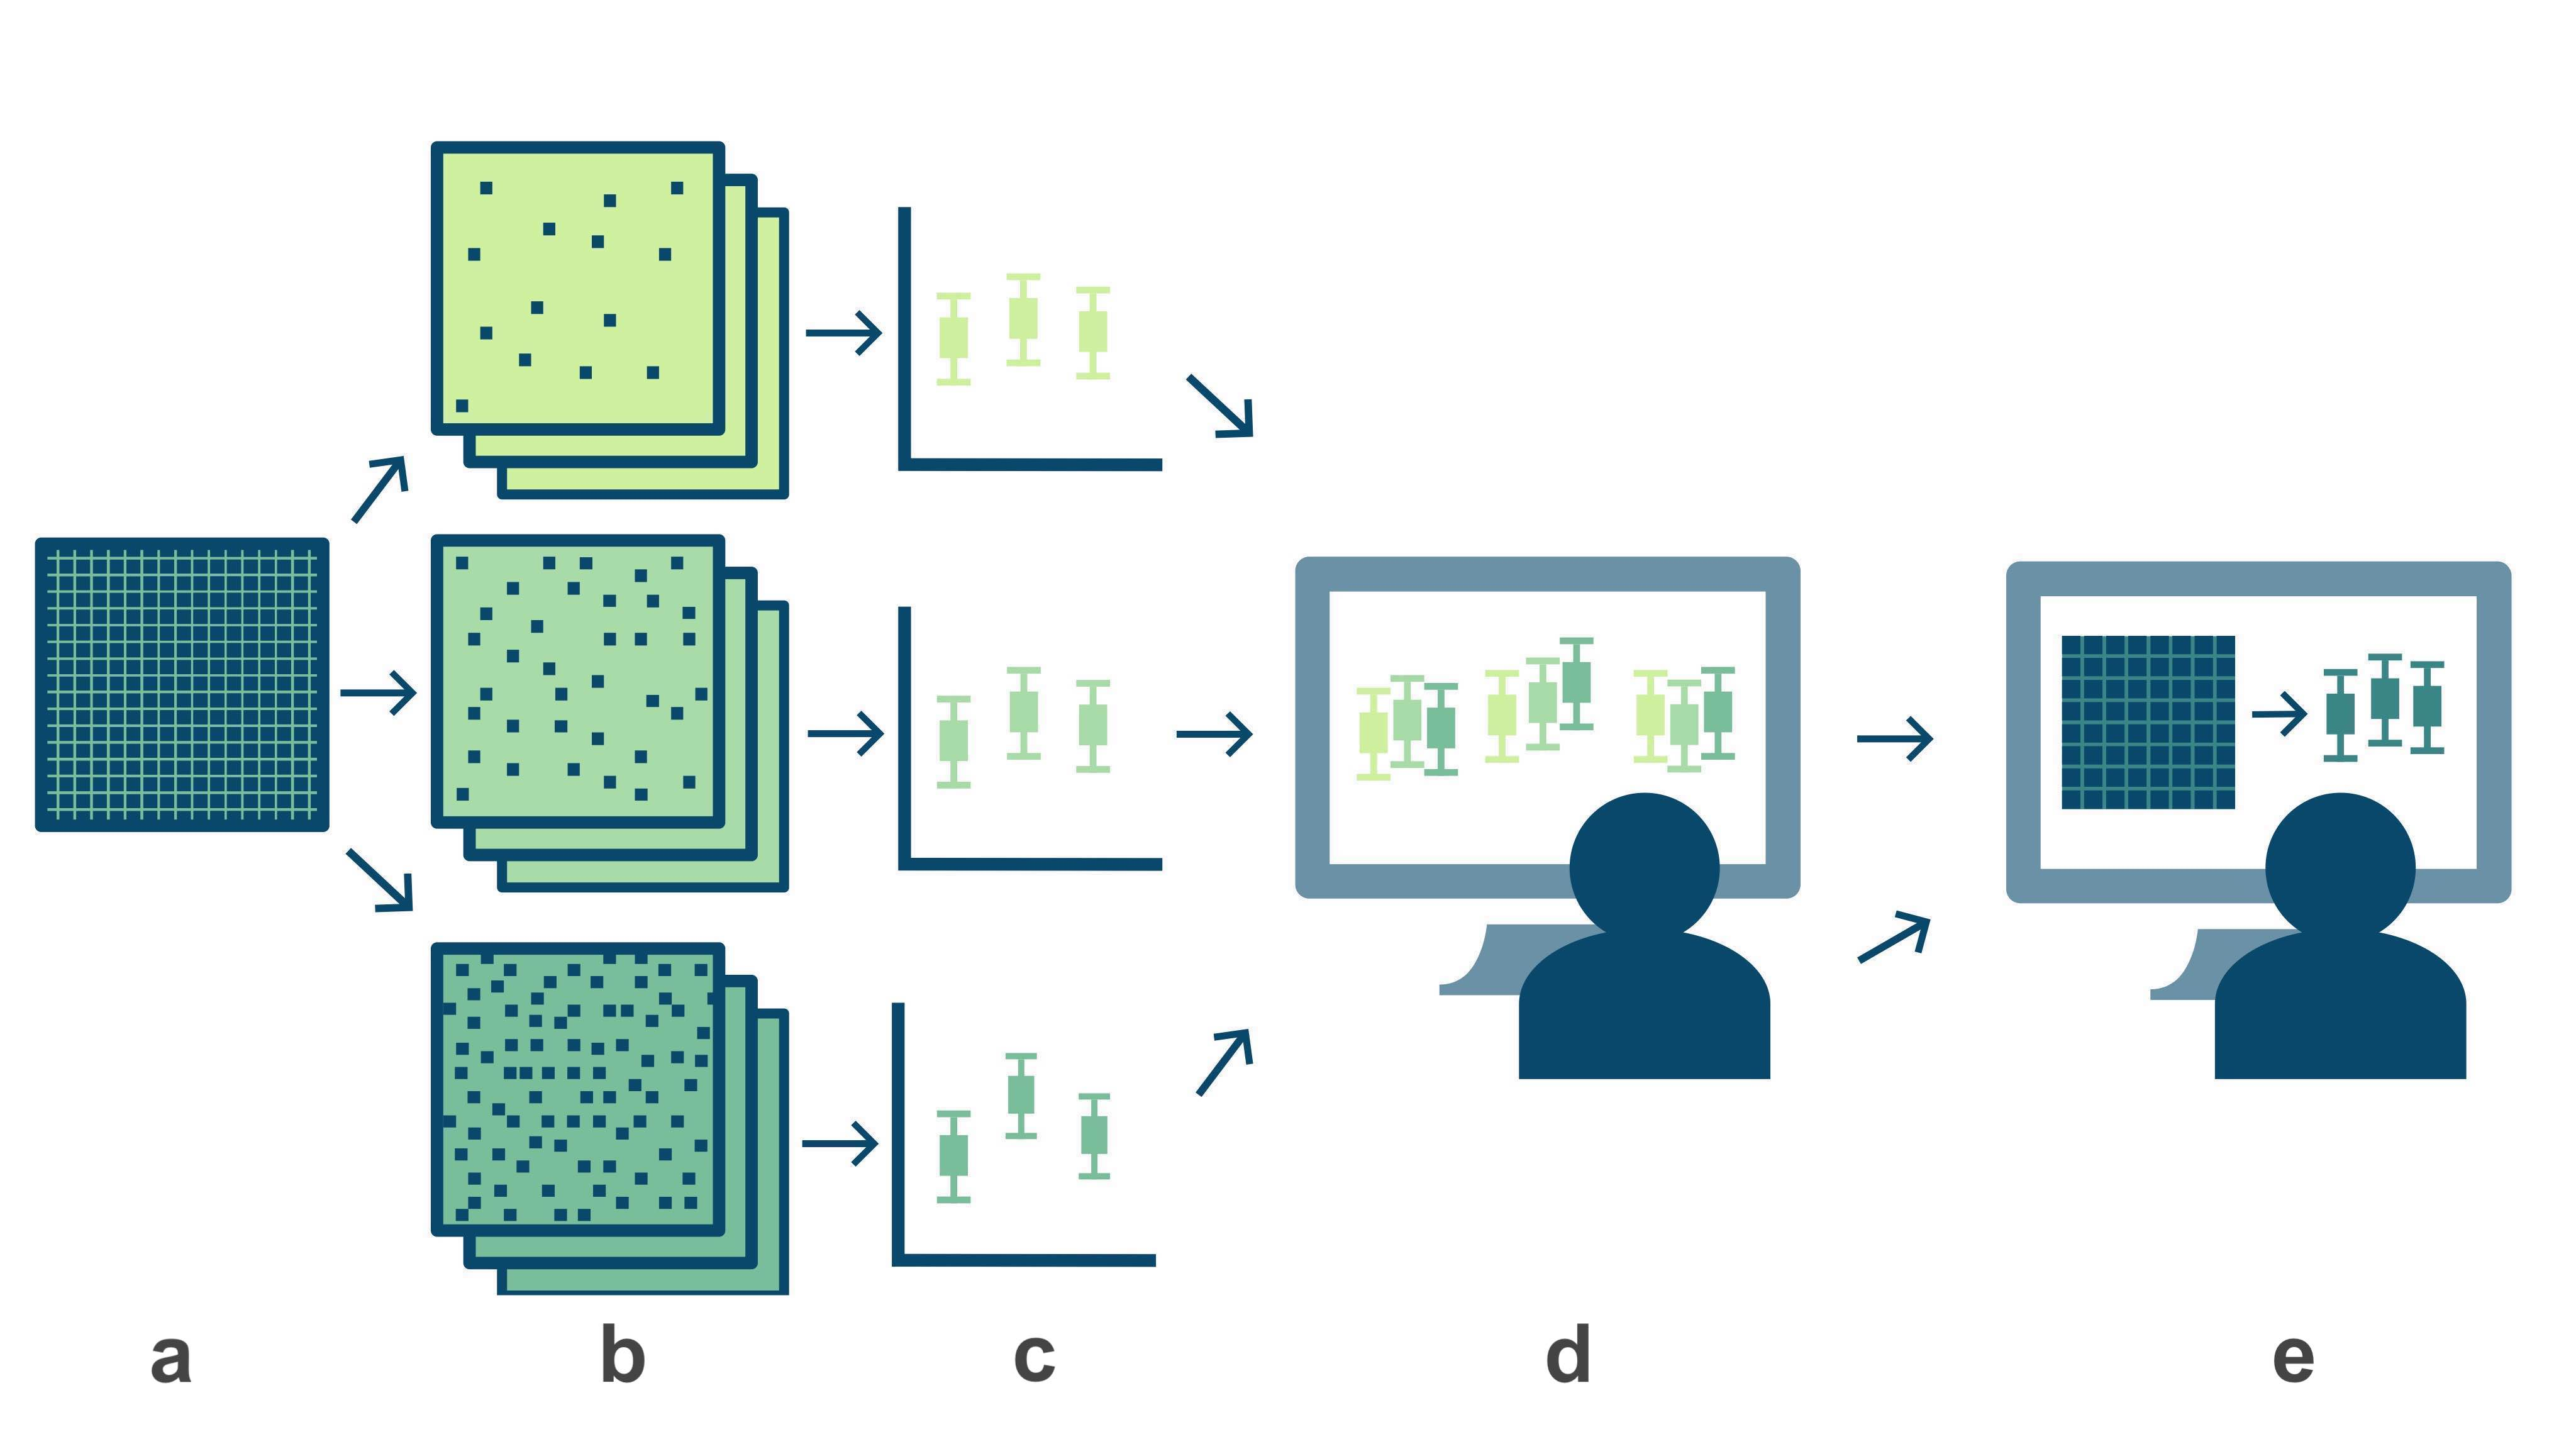
\includegraphics[width=\textwidth]{images/sampling/uncertainty_with_small_samples_labeled}
    \caption{Our proposed workflow. From the full dataset (a), a user extracts small random samples, then performs bootstrapping to extract an array of samples for each size (b). A measurement is performed on these samples, yielding estimates of uncertainty in this measurement (c). The user can inspect these uncertainties and identify patterns (d), then use their judgment to supervise training of a model that predicts the uncertainty on the full dataset (e). %(NOTE: need to reference in text.)
    }
     \label{workflow}
\end{figure}

Our contributions include:
\begin{itemize}
\item{A novel technique for efficiently estimating ``discreteness noise'' and its effect on simulation analysis.}
\item{An examination of how sample-based uncertainty prediction can be applied to simulation analysis in several fields.}
\item{A visual interface for user-supervised uncertainty prediction.}
\end{itemize}

\section{Background and Related Work}
We introduce the simulations we will use for testing and their underlying uncertainty. First, we discuss existing research related to uncertainty visualization, visual interfaces for machine learning, and simulation uncertainty quantification.

\subsection{Related Work}
Uncertainty is often identified as one of the most important challenges in visualization~\cite{curveboxplot}. There are several thorough overviews of the state of uncertainty visualization, such as~\cite{bonneau}. These summaries highlight a neglect for uncertainty in visualization research; many approaches have been proposed, but uncertainty is generally excluded from visualizations and is often seen as an afterthought, though it is crucial for scientific analysis. More work has focused on visual representations of uncertainty than on elucidating sources of uncertainty with visualization, and in particular, quantifying and modeling uncertainty is difficult and has been neglected~\cite{bonneau}.
%(cite referenced sources for this; use their related work section for a lot of sources) 
Visualizations of uncertainty must be enabled by robust quantitative analysis, which is often highly domain-specific. Here, we describe existing work in visualizing uncertainty and quantifying it for visualization.

\subsubsection{Uncertainty Visualization}
Some uncertainty work has been done from the perspective of visual analytics: tasks like data gathering, manipulation, visualization, and user perception all introduce uncertainties that users need to understand in order to properly draw conclusions from data \cite{sacha}. Researchers have created uncertainty-aware visual analytics frameworks, such as node-link diagrams enhanced with glyphs indicating uncertainty \cite{liu}. To visualize uncertainty propagation through a series of data transformations, the authors of \cite{correa2009framework} use Gaussian mixture models to model ``aggregated uncertainty'' from these transformations, enabling visualizations that show the variability in derived data with scatter plots and covariance matrices. The authors of \cite{wu} expand on this work, adding ellipsoids representing covariance for particular variables and flow trees to show the relative uncertainty introduced with each data transformation choice. 

There are many visual metaphors for uncertainty that compound on standard approaches such as boxplots and standard deviation curves. The authors of~\cite{contourboxplot} and~\cite{curveboxplot} introduce a boxplot-based visualization approach, and underlying statistical calculation, for understanding uncertainty in ensembles of curves or paths. Other modifications to standard boxplots have been proposed, such as ``functional boxplots''~\cite{functionalboxplots}, which use curves to enhance users' understanding of a data distribution and its outliers, and ``beanplots''~\cite{beanplot}, which additionally indicate the number of measurements in a sample. Uncertainty can be visualized using blurring effects \cite{haroz:seeing}. Visualizing uncertainty in physical space, such as in bounded 3-dimensional volumes, is challenging, as it can occlude other variables, and users are not used to seeing uncertainty depicted in three dimensions as they are in two \cite{haroz:2008}, \cite{li}. Color can also indicate uncertainty \cite{potter:2009}, especially in 3D space, or ``cones'' showing possible trajectories \cite{li}; the authors also employ ``magic glasses,'' allowing users to show or hide uncertainty information on top of the original data. These techniques may be more useful for expressing qualitative properties of data uncertainty than for precise quantitative analysis.

Uncertainty in scientific data, which are often multidimensional and require precise quantitative understanding, compounds on the challenges in uncertainty visualization. Simulation uncertainty is commonly analyzed by considering the results from an ensemble of simulation runs, perhaps with slightly perturbed initial conditions. The authors of \cite{potter:2009} use a variety of methods for visualizing this uncertainty in a climate model ensemble, using both spatial views (color on a map indicating standard deviation in that location; contours indicating probability levels; spaghetti plots of possible trajectories) and two-dimensional views (quartile trend charts; plume trend charts). Spaghetti plots can also be combined with glyphs representing uncertainty, and these plots can also be reimagined as graduated ribbons as in \cite{sanyal}. However, most climate ensembles do not use enough models to support such nuanced characterizations of their underlying uncertainty \cite{potter:2009}.

\subsubsection{Uncertainty Modeling}
Some nonparametric methods, which can capture outliers and noise better than parametric modeling of uncertainty can, exist, but require very fine parameter tuning~\cite{curveboxplot}. Quantitatively modeling uncertainty in physical data, such as those from scientific simulations, introduces more challenges. For example, temporal downsampling introduces uncertainty to values that are interpolated across timesteps. To address uncertainty in particle paths arising from interpolation between downsampled time steps, the authors of \cite{chen2015uncertainty} developed a polynomial-based error modeling method, using Bezier curve fitting to reconstruct physically plausible paths and visualize the results. Categorization of features, such as vortices, in simulations is often a binary choice, meaning that including uncertainty information in these classifications is difficult. The authors of \cite{biswas2015uncertainty} use fuzzy inputs and a consensus-based visualization tool to improve vortex classification in simulations.

A possible approach to modeling uncertainty from a simulation is to train a Gaussian process emulator to model a simulation using only its most influential input parameters, allowing rapid prediction of uncertainty \cite{gomez2014dissecting}. One can also use Bayesian Model Averaging to visualize the predictive uncertainty of model ensembles and individual models, as in~\cite{gosink}. Instead of calculating uncertainties and visualizing the result, representative sampling can be used to display uncertainty information to avoid occlusion while maintaining statistical properties \cite{liu2017uncertainty}. The authors of~\cite{doi:10.1029/2008WR006839} introduce a machine learning-based method for estimating uncertainty by learning the relationship between the distributions of input variables and model errors. It performs well at measuring uncertainty in a specific hydrological model, but is not capable of extrapolation, meaning that training examples must span the range of possible input variables.

%machine learning feature visualization

%specifically: ensemble visualization, flow visualization, 

%The unsupervised clustering visualization in~\cite{kwon_clustervision_2018} includes visualization of feature value distributions. (...)
\subsection{Data}
\label{data}

We use three simulations to test our uncertainty modeling method. We chose these datasets in order to highlight that our method can address different sources of uncertainty. For each simulation type, we identify a testing/training dataset and a calculation of interest. These simulations, depicted in Figure~\ref{data_examples}, have differing properties representative of the range of simulations that scientists use.


\begin{figure*}[h]
    \centering
    \begin{subfigure}{0.31\textwidth}
        \fbox{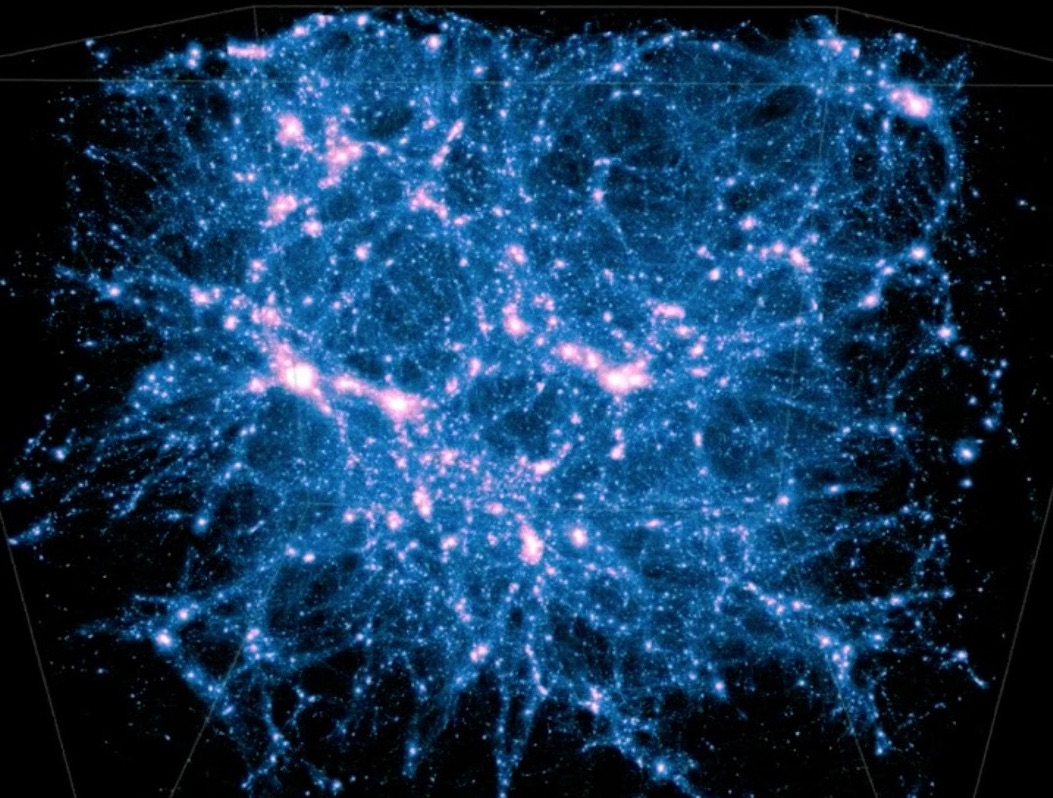
\includegraphics[width=\textwidth]{images/sampling/illustris_screenshot.jpg}}
        \caption{}
        \label{illustris_example}
    \end{subfigure}
    \begin{subfigure}{0.32\textwidth}
        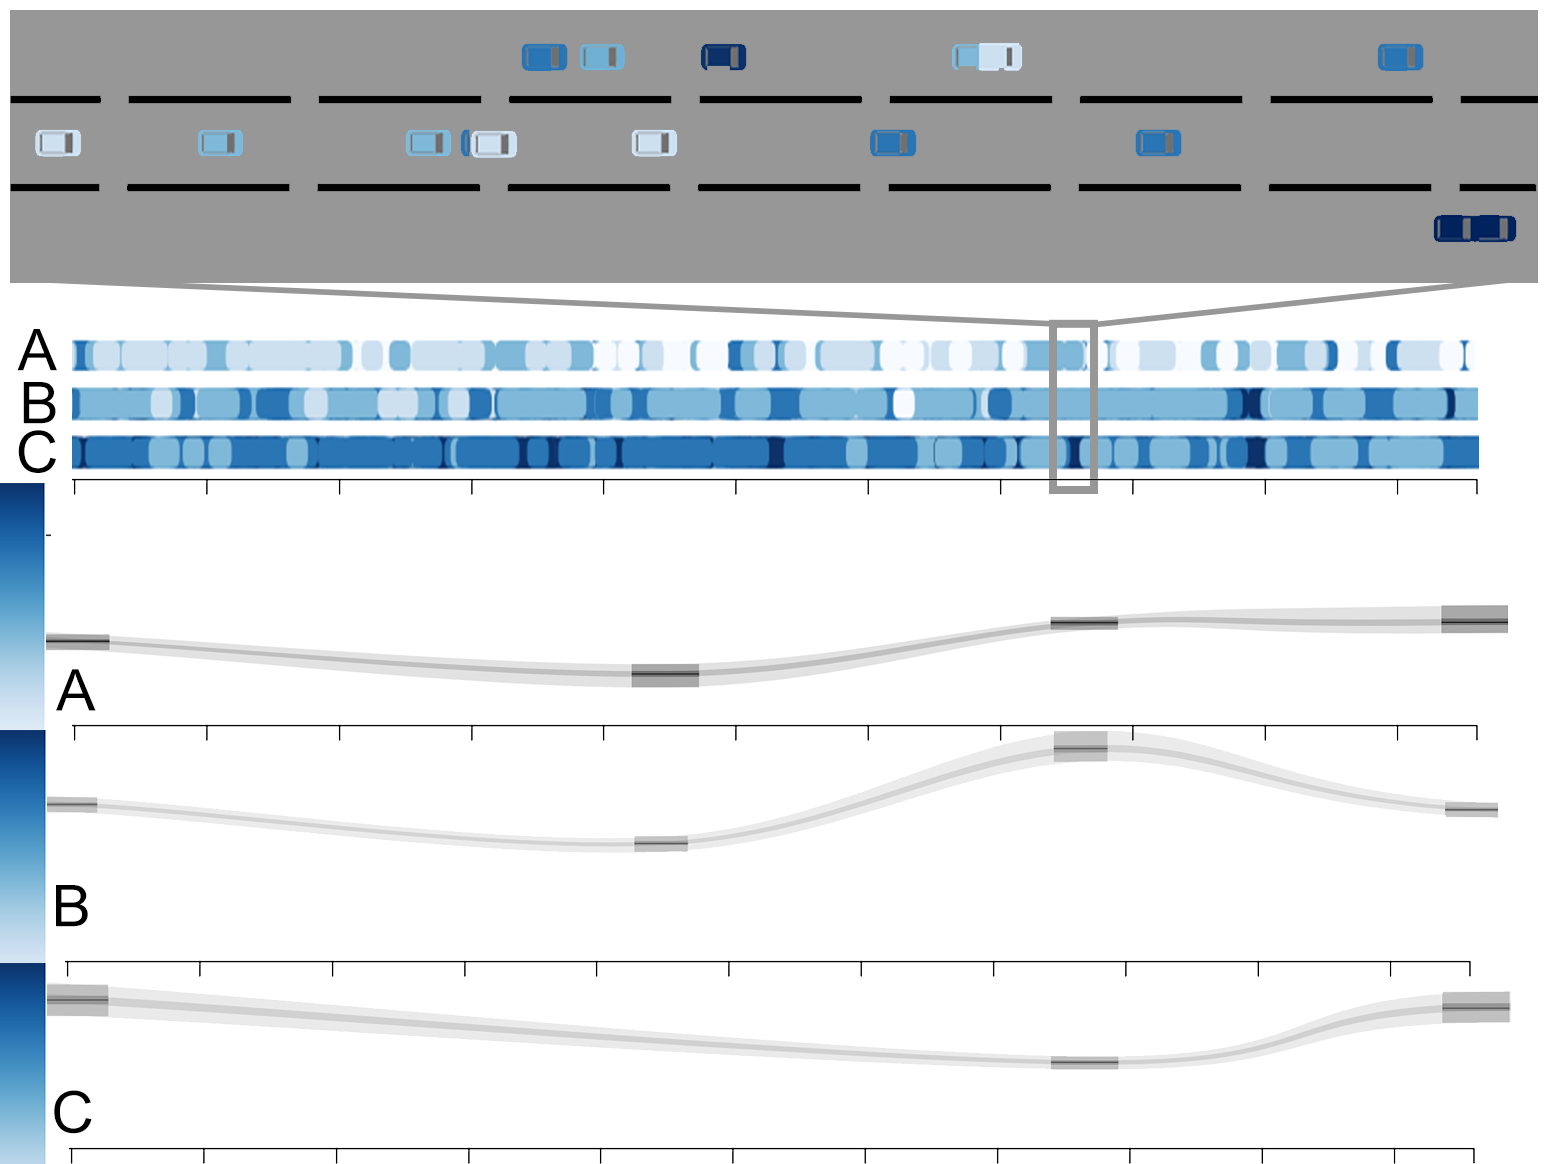
\includegraphics[width=\textwidth]{images/sampling/traffic_example_updated.png}
        \caption{}
        \label{sumo_example}
    \end{subfigure}
    \begin{subfigure}{0.32\textwidth}
        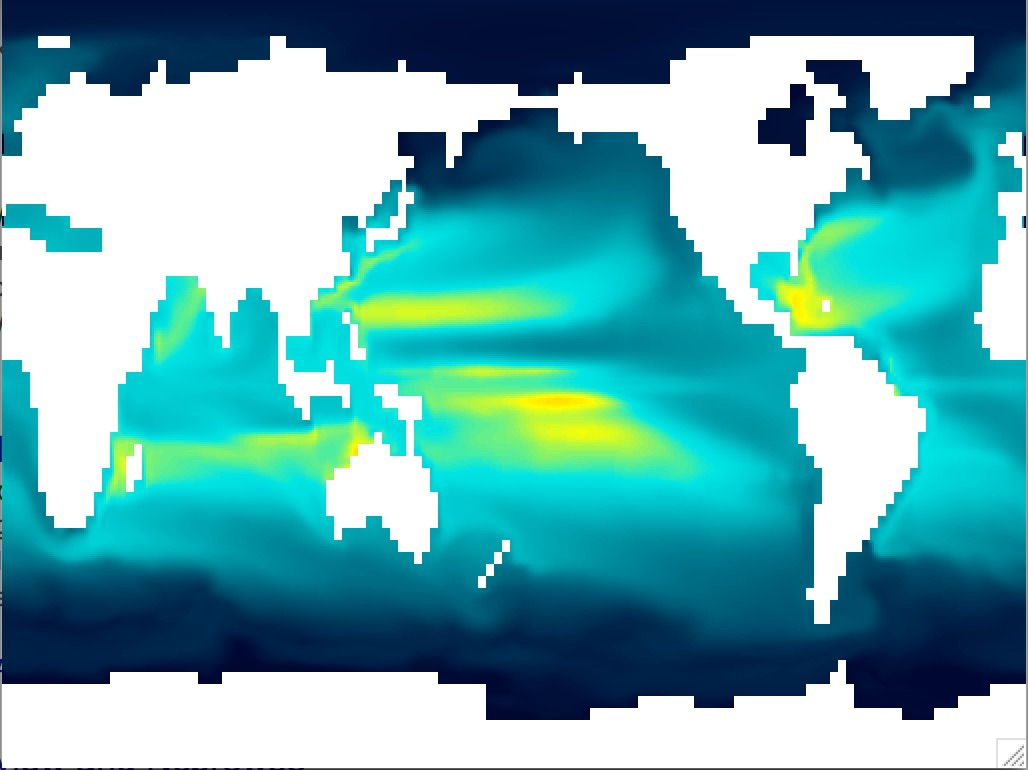
\includegraphics[width=\textwidth]{images/sampling/CanCM4_screenshot.jpg}
        \caption{}
        \label{cmip_example}
    \end{subfigure}
     \caption{Example snapshots of simulation output. (a): Dark matter particles (speed mapped to color: purple is faster) from the final timestep of an Illustris simulation. Note the halos that have formed in dense regions. (Image credit: Illustris Collaboration.) (b): One snapshot of output from SUMO for three lanes (A, B, C) along a stretch of road. At bottom, we see the average speed and its uncertainty, measured at four detector locations (one of the detectors is inactive in lane A) in one time window; in the middle, a snapshot of all the cars along this stretch of road for a single time in the window; at top, a zoomed-in view of the cars very near one detector at this time. In all sections, speed is mapped to the blue scale at left (darker is faster). (c): CanCM4, which is one of the CMIP5 models. Here, the ocean cells at a single depth level, with temperature mapped to color (yellow is warmer; blue is colder), are shown in the netCDF viewer.}
     \label{data_examples}
\end{figure*}

% emphasize the ways in which these simulations have orthogonal properties to one another:

% - different sources of discretization
% - 

% --> claim "transferability to people with the same needs" of the tool (rather than "generality") (do this a bit later in the paper)

\subsubsection{Dark Matter Simulations}
\label{dark_matter}
Our first source is Illustris~\cite{illustris_original},~\cite{illustris_release}, a suite of cosmological simulations. We downloaded the dark matter data from a single snapshot, the final timestep ($z=0$) of a dark-matter-only simulation run, Illustris-3-Dark. In N-body simulations such as these, dark matter mass distributions are represented by discrete particles. This representation approximates the continuous distribution of dark matter in the universe, creating uncertainty known as ``particle shot noise.'' Shot noise inserts uncertainty into all analyses of these simulations.

% also mention the size of the dataset we used, and the size of the biggest Illustris simulation, as well as the size of other n-body DM sims out there

Dark matter halos, which are gravitationally bound groups of dark matter particles that coalesce over time, are interesting partly because they are the environments in which galaxies form.  Algorithms that identify catalogs of halos from time-variant dark matter simulation data are called ``halo finders.'' A wide range of halo finders exists; assessing the quality of their performance is difficult, because there is no clear definition of ``halo,'' and because halos can have complex structures~\cite{behroozi}. However, the results from a halo finder determine the accuracy and usefulness of properties derived from halo catalogs. 

The ``halo mass function'' (HMF), one of these derived measurements, is a histogram of the mass distribution of dark matter halos within a simulation. Particle shot noise uncertainty, which means that the assignment of particles to particular halos is uncertain, and therefore halo masses are also uncertain, leads to uncertainty in the HMF.  Small differences in halo finder results may result in significant differences to the resulting HMFs and to ``merger trees,'' which are plots of how dark matter halos merge together over time~\cite{avila2014sussing}. (For more information on dark matter, halos, and merger trees, see~\cite{lacey1992}.)

As new surveys from telescopes measure cosmological properties to ever-greater precision, the need for accurate measurements from cosmological simulations, and understanding of their bias and uncertainty, becomes even more urgent. For comparison with sky surveys, HMFs measured from simulations need to be accurate to within 1-5 percent~\cite{behroozi},~\cite{tinker}. In order to use the HMF to observationally probe dark matter, cosmologists must continue identifying the sources of, and reducing, uncertainties in theoretical HMF measurements~\cite{murray2013}.
          
\subsubsection{Traffic Simulations}
\label{traffic_sims}
%what are traffic simulations?
% what's the source of uncertainty?
% what are we measuring and what's the significance of it?
% what are some use cases?

Our second data source is SUMO~\cite{SUMO2012}, an open source, microscopic traffic simulation. In this context, ``microscopic'' means that the behavior of each individual vehicle is simulated. SUMO simulates the placement of data-gathering detectors along roadways. Quantities available in our selected dataset include locations of detectors, time and speed of each vehicle when it passes each detector, vehicle length, and lane. Traffic model analysts use derived traffic variables, such as flow rate and vehicle density, to find \textit{spatiotemporal traffic patterns}~\cite{kerner2014introduction}. For example, using traffic models, analysts can quantify a distinction between free flow and congested traffic, then try to identify the causes of jams and congestion.

Traffic models are crucial to transportation planning in a range of situations. For example, traffic models are often used to plan for evacuations~\cite{Pel2012}. Predicted quantities can include number of vehicles involved in an evacuation, their starting points and destinations, and the traffic flow that will result from these conditions. In emergency situations, it is vital to understand the confidence in a given prediction, so that officials can make decisions based on the most likely scenarios.
Quantifying the uncertainties in traffic simulations, however, which come from inputs and from the models themselves, is challenging~\cite{traffic_volume}. One of these uncertainty sources is discretization of differential equations that describe traffic movement. To understand the likelihood of different traffic forecasts, one must understand the influence of uncertainty.
          
\subsubsection{Climate Models}
\label{climate_models}

Our third source is an ensemble of climate models from Phase 5 of the Coupled Model Intercomparison Project (CMIP5)~\cite{taylor2012overview}. Climate models are highly complex, including hundreds of tunable parameters determining the behavior of interdependent physical processes \cite{debusschere}, \cite{randall}. We select an ensemble of nine models: CanCM4, CanESM2, CCSM4, CNRM-CM5, IPSL-CM5A-LR, MIROC4h, MIROC-ESM-CHEM, MRI-CGCM3, NorESM1-ME~\cite{taylor2012overview}. Models are run according to scenarios, called ``Representative Concentration Pathways'' (RCPs), which are possible trajectories for future greenhouse gas emissions. All models in our ensemble represent RCP4.5, which is a scenario of future low-emissions climate policy~\cite{van2011representative}. These RCPs provide a manageable, intuitive set of projected outcomes to analysts and policymakers~\cite{mcsweeney}.

% talk about size of models (and that ours is smaller because we're just using ~1 variable), and potentially larger sizes of other ensembles
The choice of models making up an ensemble is a source of uncertainty.  Most often, climate scientists measure quantities and patterns by averaging over an ensemble of models (``multi-model mean'')~\cite{vavrus}. Uncertainty is defined by the spread of models around this mean \cite{deser}, \cite{georgakakos}. Information about the spread in the models, such as their standard deviation, can help quantify this uncertainty. But the choice of models to include in an ensemble also contributes to uncertainty \cite{knutti}, \cite{vavrus}. For example, results may significantly change with the inclusion of one model in place of another. If a particular model is in disagreement with the consensus of most other models, it is unclear whether to include or exclude this model: its outlier status does not necessarily mean it is wrong, and it may well be within the range of plausible outcomes \cite{mcsweeney}. There may be scientific reasons for excluding a particular model from the ensemble--if it does not realistically represent a key, known climate process--but that analysis is outside the scope of our study; our results may be applied to any group of models with any selection criteria. 

%Several approaches to quantifying this uncertainty due to model choice are outlined in \cite{vavrus}. The authors choose to strike a balance between simple and complex methods using bootstrapping (see Section~\ref{bootstrapping}). They demonstrate that the mean and standard deviation of a bootstrapped, resampled climate model ensemble provide precise information about the confidence level of a prediction. Bootstrapping the ensemble allows for far more nuanced uncertainty analysis than does simply considering the range of values in the models themselves~\cite{potter:2009}

We choose ocean heat content (OHC) for analysis because of its conceptual importance. Ocean heat content is a key indicator of climate change effects \cite{cheng}. It is also mathematically simple: calculating OHC requires integrating heat capacity over every ocean grid cell volume in a model. Therefore, we select our models from among those CMIP5 models with ocean cell volumes and ocean heat capacity data. Models have different spatial resolutions, adding another source of discretization uncertainty. It is important to assess and constrain uncertainty in OHC, as it is closely related to Earth's heat balance, which is crucial to the conclusions of climate change studies ~\cite{cheng},~\cite{gregory}. 

\subsection{Bootstrapping and Simulation Uncertainty}
\label{bootstrapping}
Bootstrapping is the process of randomly sampling a dataset with replacement. One randomly chooses elements of a dataset, allowing elements to be chosen multiple times. Some items, then, will be included more than once, and some will be excluded. Repeating this many times creates an ensemble of datasets useful for estimating variance of the source dataset~\cite{Steck}. Thus, bootstrapping provides a simple, generalizable, powerful way to quantify uncertainty. 

For example, bootstrapping techniques have been used  in~\cite{rau} to estimate the effect of particle noise in N-body simulations. Researchers use N-body simulations to study gravitational lensing, a phenomenon in which light is bent around a massive object in space. The authors of~\cite{rau} create a dataset with 100 bootstrapped resamplings, each containing the same number of particles as the original dataset; this allows them to test the effect of particle noise on the lensing in the simulation.

Bootstrapping has also been used to estimate uncertainty in measurements of climate models. As discussed in Section~\ref{climate_models}, the multi-model mean used to assess climate ensembles introduces uncertainty. The authors of~\cite{vavrus} use bootstrapping, resampling from an ensemble of 13  models, to assess the uncertainty of temperature and precipitation measurements. Similarly, bootstrapping has been used to estimate uncertainty in traffic forecasting models~\cite{RePEc:eee:transa:v:39:y:2005:i:6:p:531-547},~\cite{Brundell2000}.

Differentiating among uncertainties in climate simulation data based on their sources is quite difficult. Bayesian models may be used to determine the contribution of each source of uncertainty~\cite{northrop}, but in general, the complexity of uncertainties in interacting processes can occlude one another. Bootstrapping over the choice of models provides a conceptually elegant way to assess the effect of the model choice on uncertainty. This is true, too, for particle noise; bootstrapping will allow us to extract and quantify the uncertainty resulting from particle noise. 

A bootstrapping and sampling procedure has the advantage of being strongly generalizable. These techniques can be performed without any prior modeling of the data. Additionally, sampling can be improved on-the-fly; if a certain number of samples does not give satisfactory results, one can increase the number of samples as desired without having to start over~\cite{Cormode:2012:SMD:2344400.2344401}.

\section{Methods}
We outline the steps taken to measure and model discreteness uncertainty for each dataset, aiming to develop a generalizable procedure. 

\subsection{Sampling}
First, we extract samples of size $f$ from each dataset, for a range of values of $f \ll 1$. Table~\ref{speedup_table} shows the sample sizes used in our case studies; these samples were chosen to be small enough for significant speedup, while large enough to capture sufficient information (see Section~\ref{results}). For the particle data, we randomly select $f * n_p$ particles, where $n_p$ is the total number of particles in the simulation. From each climate model, we extract $f * n_c$ cells, where $n_c$ is the total number of ocean cells in a model, and from the traffic model, we extract $f * n_o$ observations, where $n_o$ is the number of traffic detections. While the mass per particle is constant in Illustris-Dark, the CMIP models have different numbers of ocean cells, and total ocean volumes vary. Therefore, a dark matter sample of size $f$ includes a total particle mass of $f$ times the total particle mass, while an ocean model sample of size $f$ does not necessarily have a volume equal to $f$ times the total ocean volume.

Next, we must identify the independent variables for each dataset: 
we will want to know the uncertainty at points in this parameter space.
For the halo mass function, these values are mass bins; for ocean heat content change, these are timesteps (monthly); and for average traffic speed, these are positions of detectors.

%We determine a number of domain bins, sample points, etc., for each dataset, or assign an algorithm to automate this decision. This is straightforward for the climate model data, which in our case is divided into monthly timesteps. In our first modeling attempt with the dark matter data, we set uniformly spaced mass bins. In order to ``smooth'' our input data for improved modeling---so as not to overfit the data---we set the number of bins to half as many as were automatically chosen by the yt halo finding algorithm \cite{yt}. This provided good spacing for larger mass bins, with smoothly varying values between mass bins at various sampling sizes. For the smaller mass bins, however, the measurements---i.e., the number of halos larger than these masses---had high values that varied greatly between adjacent mass bins and were wildly inconsistent depending on the sample size. Thus, we use adaptive mass binning (TO DO.)

\subsection{Uncertainty Measurement}
Next, we estimate the variance in the relevant measurement, for each sample, using the following procedure:

\begin{enumerate}
\item Use bootstrapping to resample the sample once.
\item Perform the relevant measurement (HMF; OHC; average speed) on this resampled data.
\item At each timestep/mass bin/position, measure the variance of all measurements we have taken so far.
\item Repeat (1-3) until the variance converges at most timesteps, mass bins, or positions.
\end{enumerate}

%can include table of number of resamples & epsilon values for each application + fraction.

Because the total mass in the Illustris samples varies with fraction size, we use relative mass values, first measuring the range of halo masses for each halo catalog, then dividing this range into equally-spaced steps. Through trial and error, we find that sampling masses regularly along a logarithmic scale provides smoothly varying, and consistently-shaped, halo mass functions.

Step 2 is highly domain-specific. To obtain halo catalogs for each dark matter subset, we modify the yt halo-finding library~\cite{yt} to find halo measurements at our specified mass bins. This yields, for each bootstrapping iteration, a value for halo number density at each mass bin, which is the halo mass function (HMF). 

For the climate data, we measure ocean heat content (OHC) for each bootstrapping iteration by integrating over the heat capacity for each ocean cell, then taking the multi-model mean, for each timestep. To account for the varying ocean cell volumes, we normalize these values using the ratio of the sampled volume to the total ocean volume in each model. This yields, for each bootstrapping iteration, an OHC value for each timestep. We then calculate the change in OHC with respect to a reference time, which is the format that scientists most often study.

Lastly, for the traffic data, we simply average the speeds measured at each detector in our sample, within time bins. This yields an average speed at each detector for a range of time windows.

For each of these measurements, we check the variance in each timestep or bin by plotting the variance per iteration and measuring the threshold of variance (i.e., the number of iterations N after which the range of values is within some value $\epsilon$). Once we have calculated the OHC or HMF over enough iterations to have reached convergence in most mass bins or timesteps, we store the bin/timestep, variance, minimum, maximum, and median values, and 25th and 75th quartiles. These comprise the five summary statistics of uncertainty often depicted in boxplots~\cite{brodlie2012review}. 

%FIGURE: boxplots (in my interface) of results so far for each application, or just for one if not enough space.

\subsection{Kernel Regression and Extrapolation} 
\label{methods}
%this section most recently edited by yiran:
Next, we aim to learn a model, $\mathcal{M}$, for predicting the uncertainty of each measurement on the full datasets, using the information we have gathered as input:
\begin{equation}
\mathcal{M}(u_f, f, x) = u_{1.0}(x)
\end{equation}
where $u_f(x)$ is the uncertainty at $x$ (i.e., some timestep or mass bin) for fraction $f$. We represent uncertainty using the \textit{five-figure summary} of distributions found in boxplots: minimum, maximum, median, lower quartile, upper quartile. To reduce the dimensionality of the problem, we learn five models, one for each of these quantities. Ideally, we can save a model, once learned, then use other datasets---for example, samples from a similar simulation run---as input. 

	To predict the value of responses, given predictors, and estimate the associations among predictors and responses, one can use regression techniques. Our predictors are the uncertainties of a small data subset, and our responses are the ground truth (the uncertainties of the corresponding full dataset.) Parametric regression fits a functional form to the model inputs and outputs. This would be conceptually elegant for inserting new data into the model inputs and calculating the outputs. However, choosing a functional form to fit would be difficult without intuition for what shape the uncertainties of a dataset should take. Nonparametric modeling has the advantage of more degrees of freedom, sacrificing the elegance of a functional form---which may not be generally applicable to many types of scientific data---for greater predictive power. 

%NOTE: how do we allow substitution of a new dataset into the model?
%%%
One difficulty is that our model requires extrapolation. That is, the inputs for $f$ include values $f \ll 1.0$, but we would like to predict the output at $f = 1.0$, far beyond the range of inputs. In our case, extrapolation is motivated by the fact that the ground truth's uncertainty-related values usually share a similar pattern with those values for smaller fractions (see results in Section~\ref{results}.)

Recent work~\cite{pmlr-v28-wilson13}~\cite{WilsonGCN14} explores the challenge of extrapolation, proposing fast kernel-based regression approaches for performing extrapolation. However, the distance between training and testing inputs in our case is especially long; additionally, we expect that the uncertainty (both its magnitude and its relative values) can be strongly dependent on the sample fraction. This burdens even the best methods for predictions based on spectral mixture kernels. 

%\subsubsection{Data Preprocessing}

%First, we determine how to scale the uncertainty-related values (minimum, maximum, median, lower quartile, upper quartile) and the independent variables. 
% For example, a linear regression was performed for each fraction after the HMF data was logarithmized. 
%(NOTE: we didn't have to do this step for the other applications.)
%In order to make a clear distinction between the effects of two input variables, the linear regression parameters were recorded and then used for normalization. Mathematically, the linear regression equation for fraction $f_i$ is:

%\begin{center}
%$log(u_{f_i}) = A_ix + b_i, i = 0, 1, 2, \dots, n,$  
%\end{center}

%where $x$ is the mass bin index, and $n$ is the number of input fractions. In order to eliminate the influence of fractions on the other input feature, the mass bin indices, the data was then normalized to be of the same linear equation:

%\begin{center}
%$u'_{f_i} = (log(u_{f_i}) - b_i) \times (A_0/A_i) + b_0$
%\end{center}

To improve the extrapolation performance, we tested different ways of scaling the model parameters, ultimately making choices based on trial and error. We aim to bring the features near enough to accommodate kernel learning in the following step, but not to distort the data so much that floating point arithmetic becomes a factor. Our interface is designed to assist users to make these scaling choices (see Section~\ref{vis}) based on simple equations. For each case study, we scaled the sizes with equations of the form $\mathrm{scale}_{\mathrm{f}}(f) = \mathrm{log}(f^{1/c})$. Depending on the domain, the independent variable (such as mass) may also be scaled in order to serve as a consistent reference for different sample sizes.

To train the model with sampled data, we use pairs of sample uncertainty as the ``input'' and ``output'':

\begin{equation}
%\begin{align}
%\begin{split}
\mathcal{M}(\mathrm{v}_f, \mathrm{scale}_{\mathrm{frac}}(\mathrm{input\textunderscore frac}), \mathrm{scale}_x(x)) = \mathrm{v}_{\mathrm{output\textunderscore frac}}(x)
%\end{split}
%\end{align}
\end{equation}

for each value, $v$, representing uncertainty being predicted. In this study, the values used are the minimum, maximum, median, lower quartile, and upper quartile. To make predictions, we will use the model in Equation 2 with the output fraction set to 1.0 and the input being the array of training samples. 

%A scheme was designed to assist the user in defining the scaling method. Choices of exponent $c$ are made by the user, and then a scaling process and a linear regression was performed based on the chosen exponent. The efficiency of the scaling process is then illustrated by the RMSE of the regression.

\subsubsection{Prediction}
We first arrange input fractions and independent variable indices of the training samples as data points on a grid. We adopt gaussian process methods for extrapolation, closely following the method in~\cite{pmlr-v28-wilson13}. A kernel (covariance function) is selected to represent the distribution of a set of functions, and then a posterior is generated according to the training data. Based on the posterior distribution, predictions are made for the ground truth data.

% don't know whether the formulae are needed here
The spectral mixture kernel, $k_{SM}$, we use is:
\begin{center}
$k_{SM}(x, x'|\theta) = $$\sum_{q=1}^{Q}$$w_q^2\frac{|\Sigma_q|^\frac{1}{2}}{(2\pi)^\frac{D}{2}}\exp(-\frac{1}{2}||\Sigma_q^\frac{1}{2}(x - x')||^2)$\\ 
$\times\cos(x - x', 2\pi\mu_q),$
\end{center}

where $\theta$ represents all of the kernel hyperparameters, and one SM kernel is defined and initialized for each input dimension. To learn the hyperparameters, we maximize the log marginal likelihood:
%The hyperparameters can be learned by maximizing the log marginal likelihood:
\begin{center}
$\log(p(y|\theta, X))\propto -[y^\mathrm{T}(K_\theta + \sigma^2I)^{-1}y + \log|K_\theta + \sigma^2I|].$
\end{center}

%We also don't want very different fractions to be too close to one another. 
%to add: is there a way to know while we're tuning this that our choice is a good one? any information available?

%IMAGE: optimized scalings in the interface, for one example.

%discuss multi-scale properties/difficulty:

%Some of these quantities change with varying subset sizes, such as mass, halo number density, and the magnitude of ocean heat content, while some, such as timesteps, don't. Downsampling the data means that though the variance of a quantity in a subset may be roughly proportional to the variance of that quantity in the full dataset, the absolute values will not be the same. For example, when we downscale, the range of halo masses decreases. For our model, we'd like to convert between these masses to the masses found in the full dataset. This will be true of any property that is directly affected by downsampling, such as number densities. Ideally, this scaling can be hidden within the model, which will learn the relationship between input and output values. However, we may have to explicitly scale values if the models do not address this adequately (TO DO).

We run each model to make five predictions, one for each value in the uncertainty spread (five-figure summary). %(Note: is there a better way to learn a distribution??) 
To apply the trained model to a new dataset, such as another simulation run using different parameters, we save the learned parameters and apply them to the new dataset. See section~\ref{ohc_case_study} for an example result.

\subsection{Visualization}
\label{vis}
%THESIS OF THIS SECTION: visualization is crucial to the applicability of our tool. our method is fast so that it enables real-time prediction, and visualization facilitates exploring this prediction AND it also facilitates tuning to more-precise predictions if desired.

%boxes showing convergence quality: striking the balance between too much information -- can have infinite layers of uncertainty if we look hard enough -- and just hinting at the relevant information.

%make sure to gather sources that specifically pertain to this section.

% list what we want users to be able to do/see in our visualization:
Visualization enables the full usefulness of our approach. Through a flexible interactive interface, users can take advantage of its fast prediction and interactive tuning to efficiently explore their own data. Moreover, much of our method's benefit is qualitative: learned patterns in the uncertainty reveal themselves quickly through visualization. Scientists who work with simulations confirm that this kind of information is highly useful (see Section~\ref{uwp}).

Our visualization should enable users to answer the following questions: What is the predicted uncertainty? How confident can we be in the prediction? What are the patterns in uncertainty, depending on sample size? If we change the input, for which values is uncertainty most affected?

Additionally, it should show users enough information so that they can guide the training of an accurate uncertainty prediction model. Our interface contains panels for selecting input data, scaling and optimizing features for modeling (Figure~\ref{control_panel}), and viewing sampled and predicted results (see Figure~\ref{hmf_case_study}). 

%In the left panel, users choose sample sizes to extract, and specify which to include in the model. In the middle panel, we display the distributions of features to be included, allowing the user to scale these distributions as desired. Finally, the panel on the right shows uncertainty measured from the subsamples, and/or the predicted ``true'' uncertainty, in a boxplot-style representation. We indicate confidence in each prediction with a grayscale box representing convergence of uncertainty values for that bin; darker gray corresponds to higher confidence (i.e., better convergence).

The ``control panels'' (Figure~\ref{control_panel}) facilitate all the steps leading up to an uncertainty prediction. First, the user can load a dataset and specify the sizes of samples they wish to extract. Then, the user can ask to perform a measurement of interest by pressing ``calculate.'' This performs the measurement, such as halo mass function or ocean heat content, repeatedly, keeping track of the variance in the results. The calculation is repeated until satisfactory convergence is reached in a majority of the mass bins or timesteps (the desired convergence threshold can be changed as needed).

Once the calculations are performed, the resulting measurement and its uncertainty is shown in colored boxplots, as in Figure~\ref{hmf_case_study}. These can be viewed individually or stacked, with one color representing each sample size. Beneath the boxplots, a box indicates the quality of the prediction (based on the convergence of the variance measurements), with darker gray  indicating higher confidence. The right side of the control panel now shows the distribution of each relevant variable (see Figure~\ref{control_panel}). At this point, users can choose to scale these features, which become inputs into the prediction model, either by using default log scaling, or by typing in the scaling they prefer. This scaling should bring input features closer together for better regression results (see Section~\ref{methods}). In our case studies, we focus on scaling the ``size'' feature.

%\begin{figure}[h]
%    \centering
%    \includegraphics[width=0.45\textwidth]{placeholder_sample_ohc.png}
%    \caption{Our prototype interface. In the left panel, users choose sample sizes to extract, and specify which to include in the %model. In the middle panel, we display the distributions of features to be included, allowing the user to scale these distributions %as desired. Finally, the panel on the right shows uncertainty measured from the subsamples, and/or the predicted ``true'' uncertainty, in a boxplot-style representation. We indicate confidence in each prediction with a grayscale box representing convergence of uncertainty values for that bin; darker gray corresponds to higher confidence (i.e., better convergence). (See Figure~\ref{hmf_predicted} for another, larger interface image.)}
%     \label{ui}
%\end{figure}

Once the array of samples is chosen and the features are scaled, the user can choose ``update prediction'' to train the model and view the predicted uncertainty (for example, as in Figure~\ref{hmf_predicted}).

\begin{figure}[h]
    \centering
   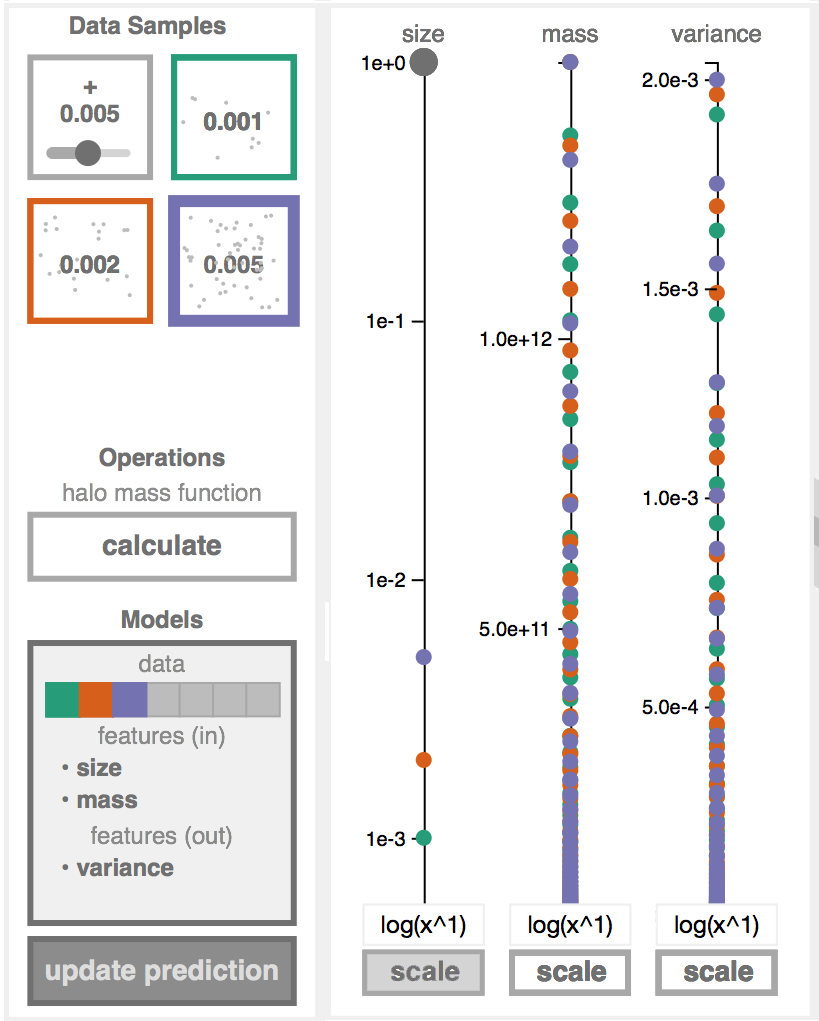
\includegraphics[width=.3\textwidth]{images/sampling/control_panel.png}
    \caption{The ``control panels'' for our interface. On the left, users can choose the sizes of data samples to extract; the ``models'' show which samples and which features are included as input and output to the model to be trained. On the right, the user has scaled the ``size'', or input fraction, parameter.}
    \label{control_panel}
\end{figure}

The default appearance is important, because users might be dissuaded if they have to perform complex interactions before seeing a meaningful result. The fine tuning of our regression model depends on several choices, but the basic implementation of our approach (see Section~\ref{methods}) can provide an estimate of the uncertainty without supervision. We show this estimate by default, allowing the user to then modify feature scalings to optimize the prediction.

% talk about UI components

% talk about problem of comparison

% talk about problem of multiple scales

% TO DO: talk about how to highlight changes

\section{Results and Applications}
We evaluate our method and visualization tool through interviews with scientists working on simulations and three case studies. First, we establish the current work practices of scientists working with simulations, including understanding any visualization tools they use and what needs are not met by those tools. Then, we aim to understand which capabilities of our tool would be useful to them, and the scenarios in which they might use it. Finally, we demonstrate the use of our method and tool on three representative datasets (described in Section~\ref{data}).
%emphasize transferability to people with similar analysis needs

%What's the advantage, if any, of looking at the uncertainty for the measurements on the subsets?


%NOTE: we could discover that the results aren't good in ___ domain but are good in ___ domain (hopefully), and that the application makes sense in ___ domains but not ___ domains, and those may not be the same categories. but if we present those results systematically, it will be convincing.

\subsection{Understanding Work Practices}
\label{uwp}
% cite sources to justify how we did evaluation:
% - "a systematic review on the practice of evaluating visualization"

% identify state-of-the-art for quantifying this type of uncertainty in each field, and qualitatively compare

% to be strong, we need to assess both visualization and data analysis process, with emphasis on the latter

\label{hmf_case_study}
\begin{figure*}[h]
      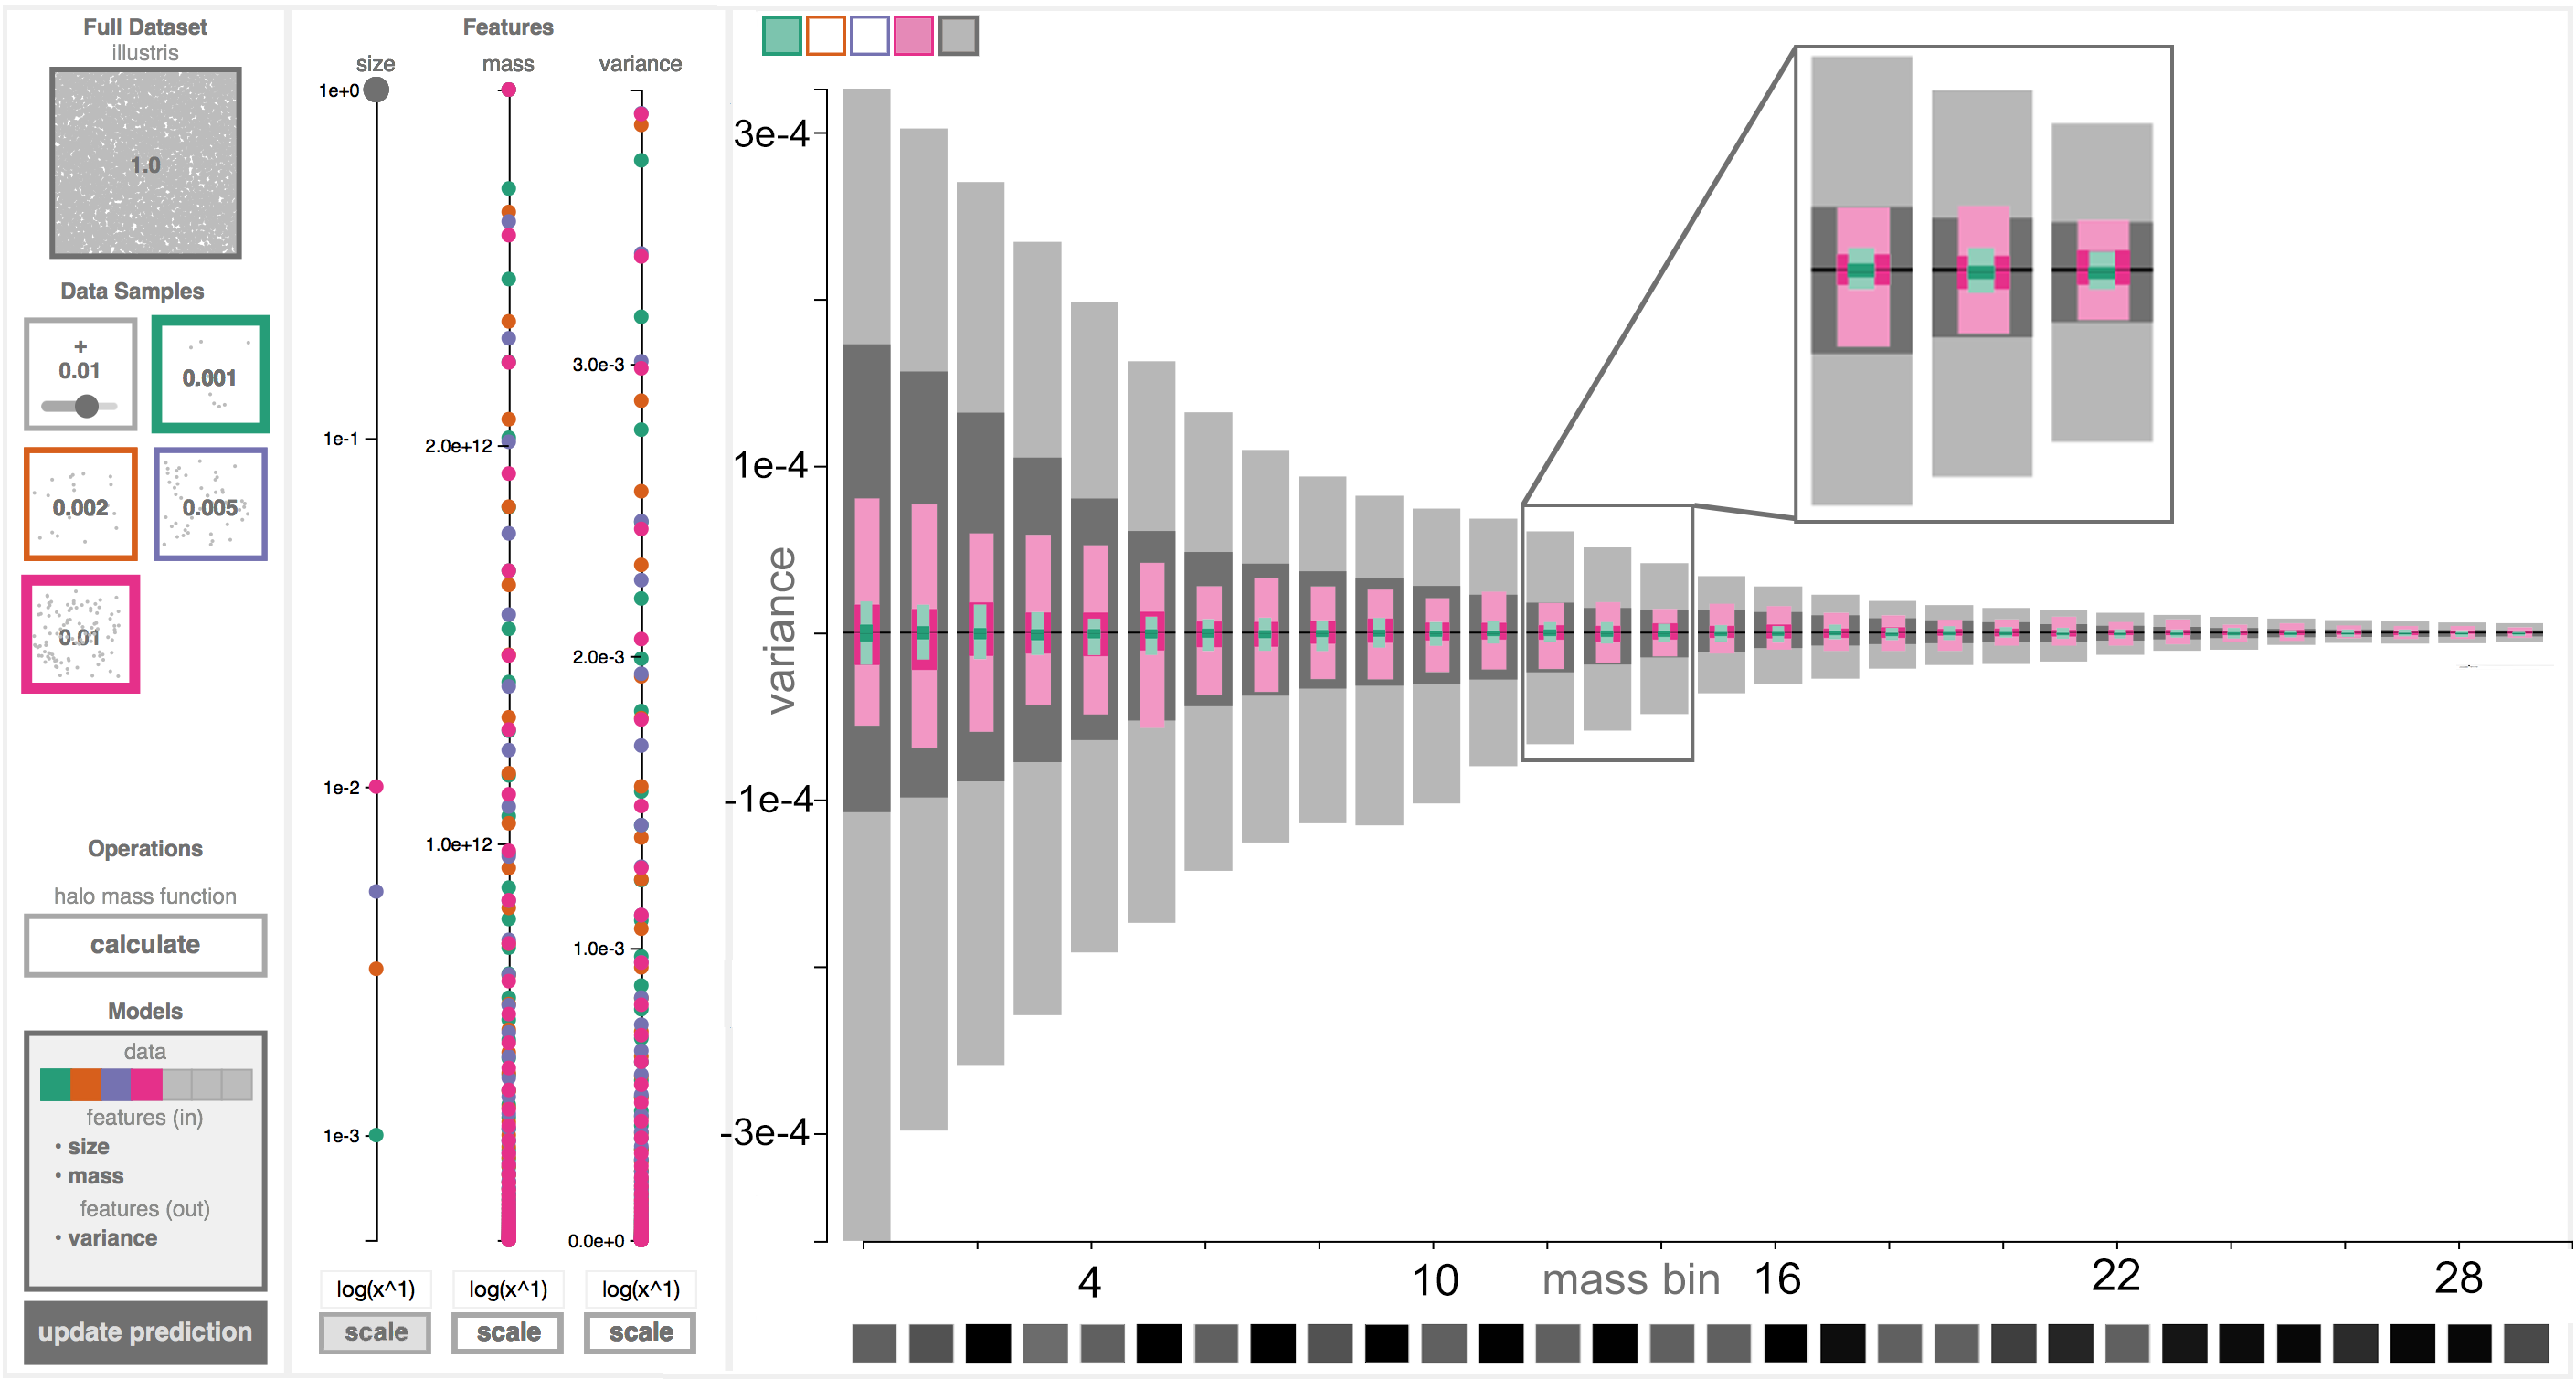
\includegraphics[width=\textwidth]{images/sampling/hmf_prediction_case_study.png}
     \caption{Prediction, and sampled uncertainties, for the dark matter halo case study, shown in our full interface. At left, we see the set of samples the user has chosen. The user has highlighted two samples to show in the uncertainty view. In the middle panel, we see that the user has scaled the ``size'' values as input into the prediction model. At right, we see the measured uncertainties for the samples (pink, green), and the predicted uncertainties (gray), shown in stacked boxplots. Because the halo mass function spans several orders of magnitude, it is difficult to show in one view; instead, we are showing the boxplots centered around their medians for each mass bin. The quality indicator boxes on the bottom of the right panel show that most predictions have a very high confidence. (Axis labels are enlarged for display purposes.)}
     \label{hmf_predicted}
\end{figure*}

To assess the potential usefulness of our approach and visualization tool, we consulted with domain experts who work with climate models and dark matter simulations. Specifically, we spoke with: one Cosmology researcher at a university, in person, who primarily works on N-body dark matter simulations; one Cosmology researcher at a university, in person, who works with observational data but in tandem with other researchers using simulations; one Atmospheric Science researcher at a national laboratory, in person, who primarily works with ocean dynamics in climate models; one Atmospheric Science researcher at a university, over e-mail, who primarily works with ensembles of climate models.

We held these conversations with the goal of understanding common work practices in fields for which simulations play a crucial role. According to a recent survey of evaluation practices in visualization~\cite{6634108}, process-based evaluation such as understanding work practices is crucial yet under-utilized. Through this analysis, we can draw a clear link between our method and tool and the real-world scientific problems it may be applicable to solving.

\subsubsection{Current Tools}
None of the interviewees currently uses visualization tools beyond those offered in R or Python libraries. Several expressed that visualization software is never used in their peer groups, or that visualization is an afterthought, especially for analysis. The reason most cited for this was time, but also lack of a flexible enough tool; one had tried to use ParaView but felt he was unable to use it to show derived properties of his data, and especially not to show uncertainty.

They are all familiar with boxplots or contour plots for conveying uncertainty, and some produce these plots themselves. One person mentioned that he creates his own ``animations'' from series of Python-generated plots. In general, they perform their own statistical analysis using generic packages in R or Python. One atmospheric scientist expressed that the current level of formality in his analysis varies widely, depending on the case; sometimes, statisticians might help with a problem, but they are unlikely to have any expertise in climate modeling. One researcher mentioned using machine learning to explore the parameter space of simulation inputs (see below).

\label{traffic_case_study}
\begin{figure*}[h]
    \centering
    \begin{subfigure}{0.32\textwidth}
        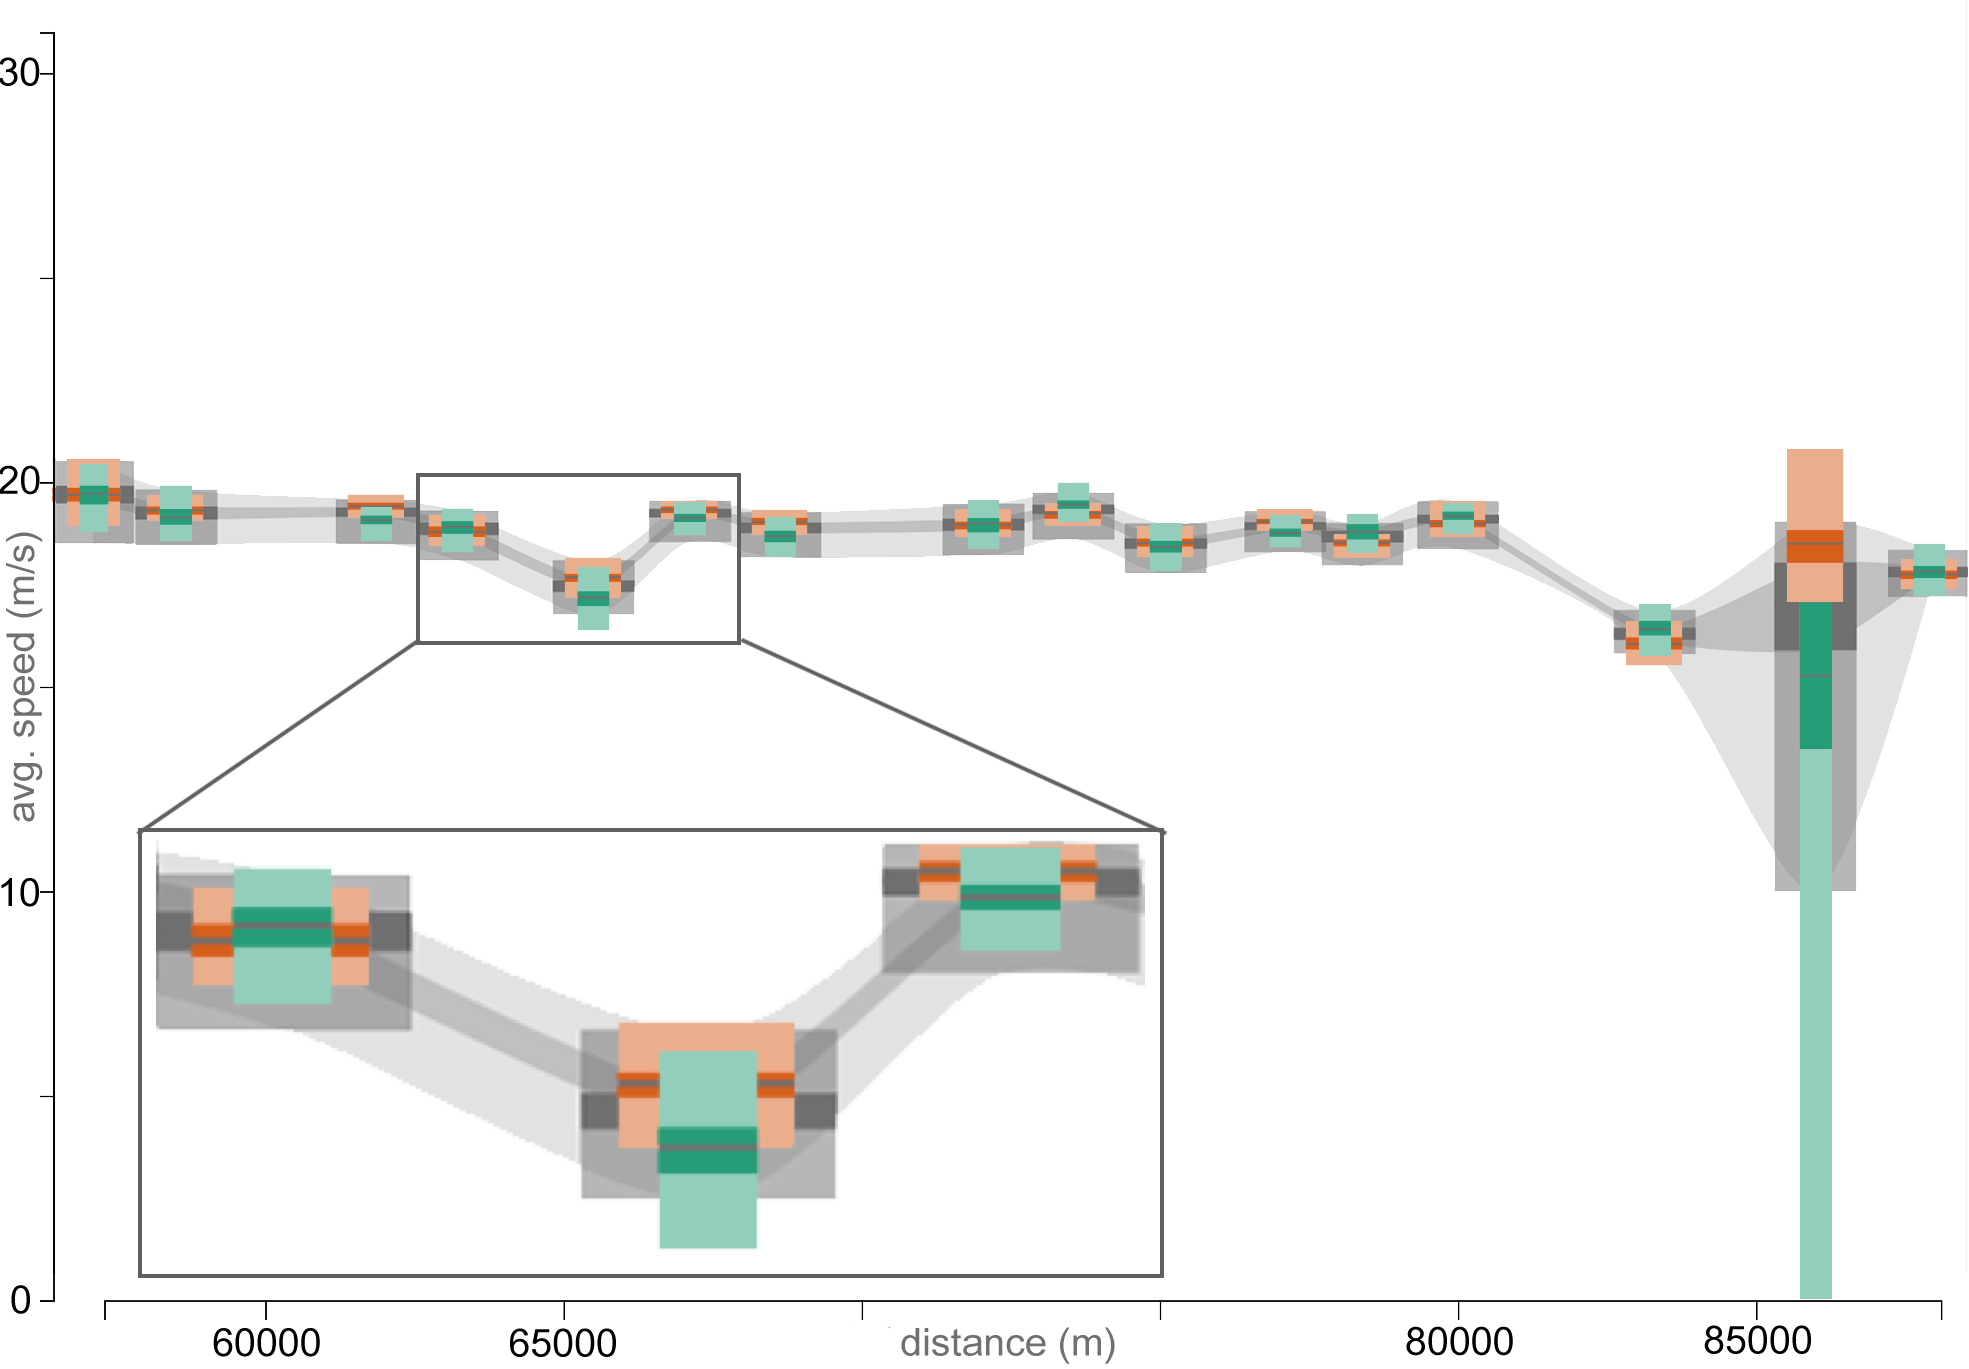
\includegraphics[width=\textwidth]{images/sampling/timestep_a_samples_predicted.png}
        \caption{Time window 1.}
        \label{fig:a}
    \end{subfigure}
    \begin{subfigure}{0.32\textwidth}
        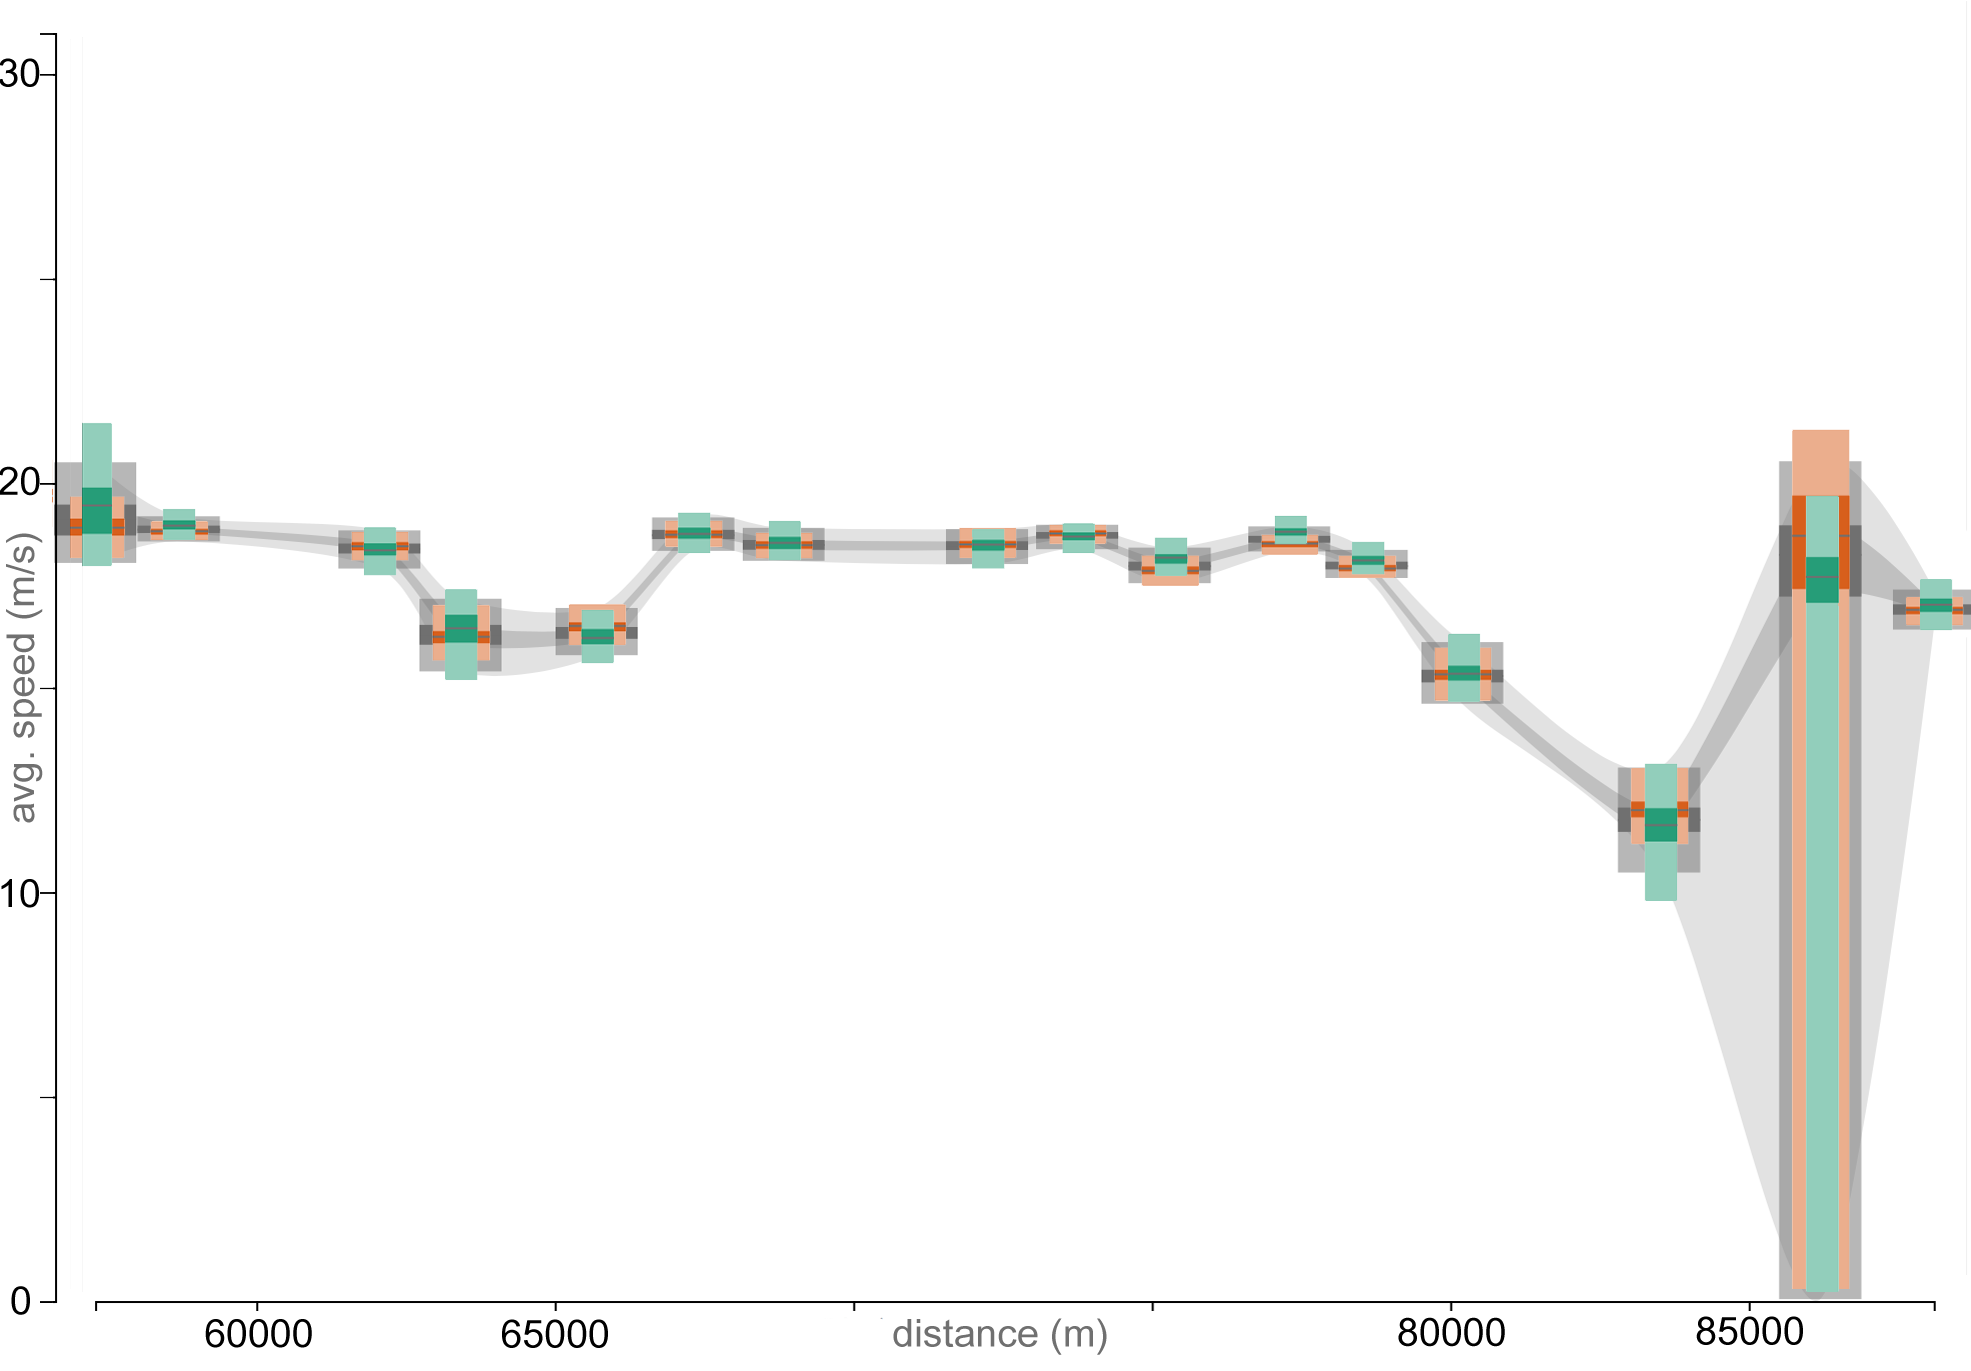
\includegraphics[width=\textwidth]{images/sampling/timestep_b_samples_predicted.png}
        \caption{Time window 2.}
        \label{fig:b}
    \end{subfigure}
    \begin{subfigure}{0.32\textwidth}
        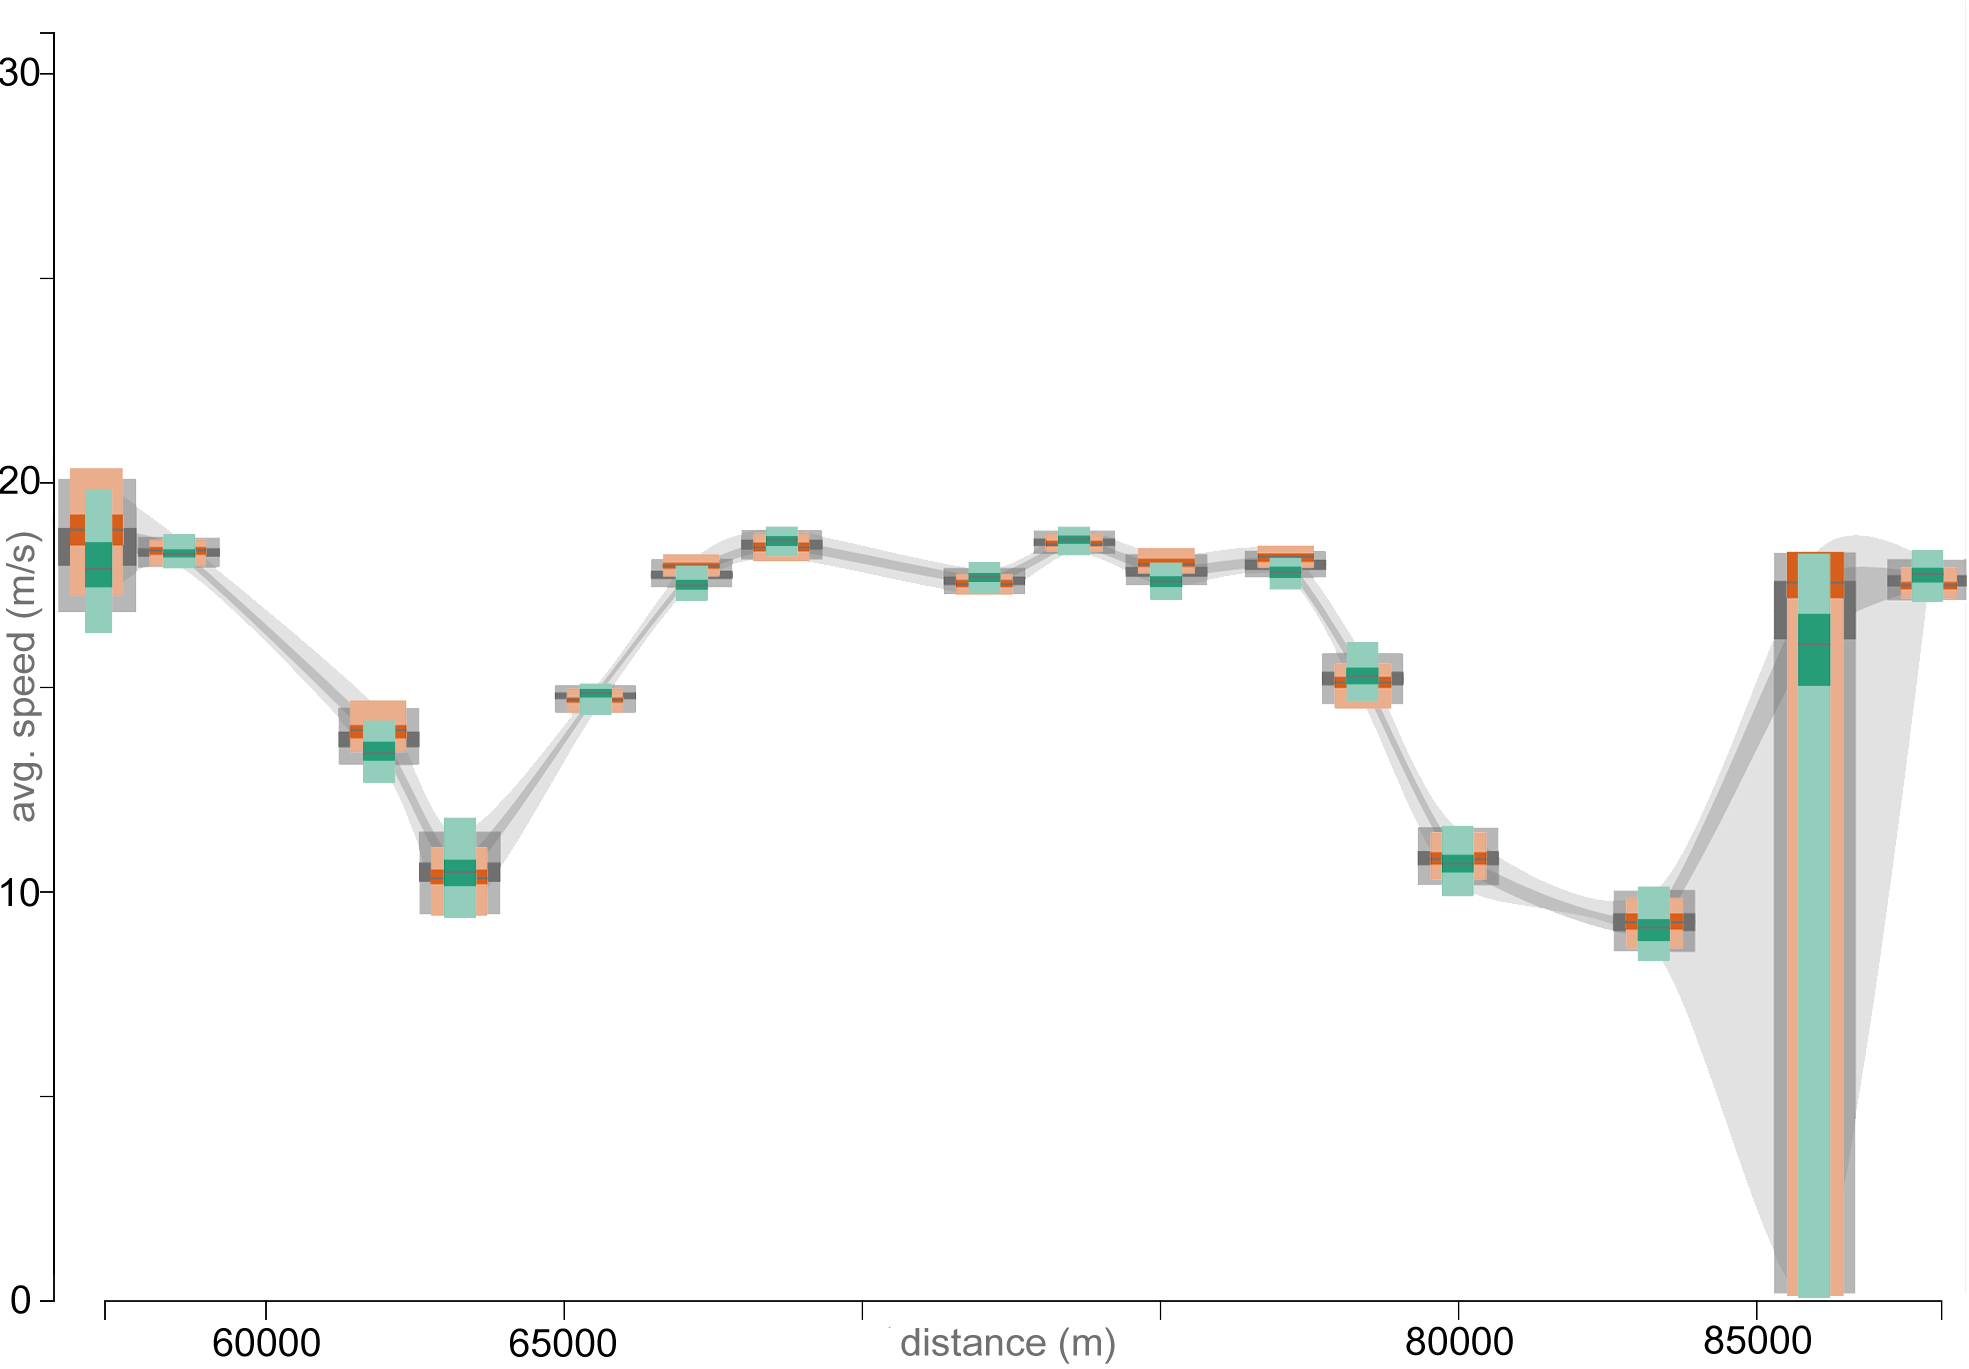
\includegraphics[width=\textwidth]{images/sampling/timestep_c_samples_predicted.png}
        \caption{Time window 3.}
        \label{fig:c}
    \end{subfigure}
     \caption{Average speed and uncertainty for samples with sizes 0.05 (green) and 0.1 (orange), and the predicted uncertainty (gray, connected by an interpolated curve), for three consecutive time intervals. The interpolated curve of predicted values helps discern the path of a time series, especially when the samples are unevenly spaced, as in this example. The inset box in (a) shows the overlaid boxplots in detail. Here, the green box, representing sample size = 0.05, represents the median (middle gray line), upper/lower quartiles (darker green), and min/max (lighter green). Similarly, orange ($f=0.1$) and gray (prediction, $f=1.0$) boxplots are stacked behind.}
     \label{traffic_predicted}
\end{figure*}

\begin{figure*}[h]
    \centering
    \begin{subfigure}{0.32\textwidth}
        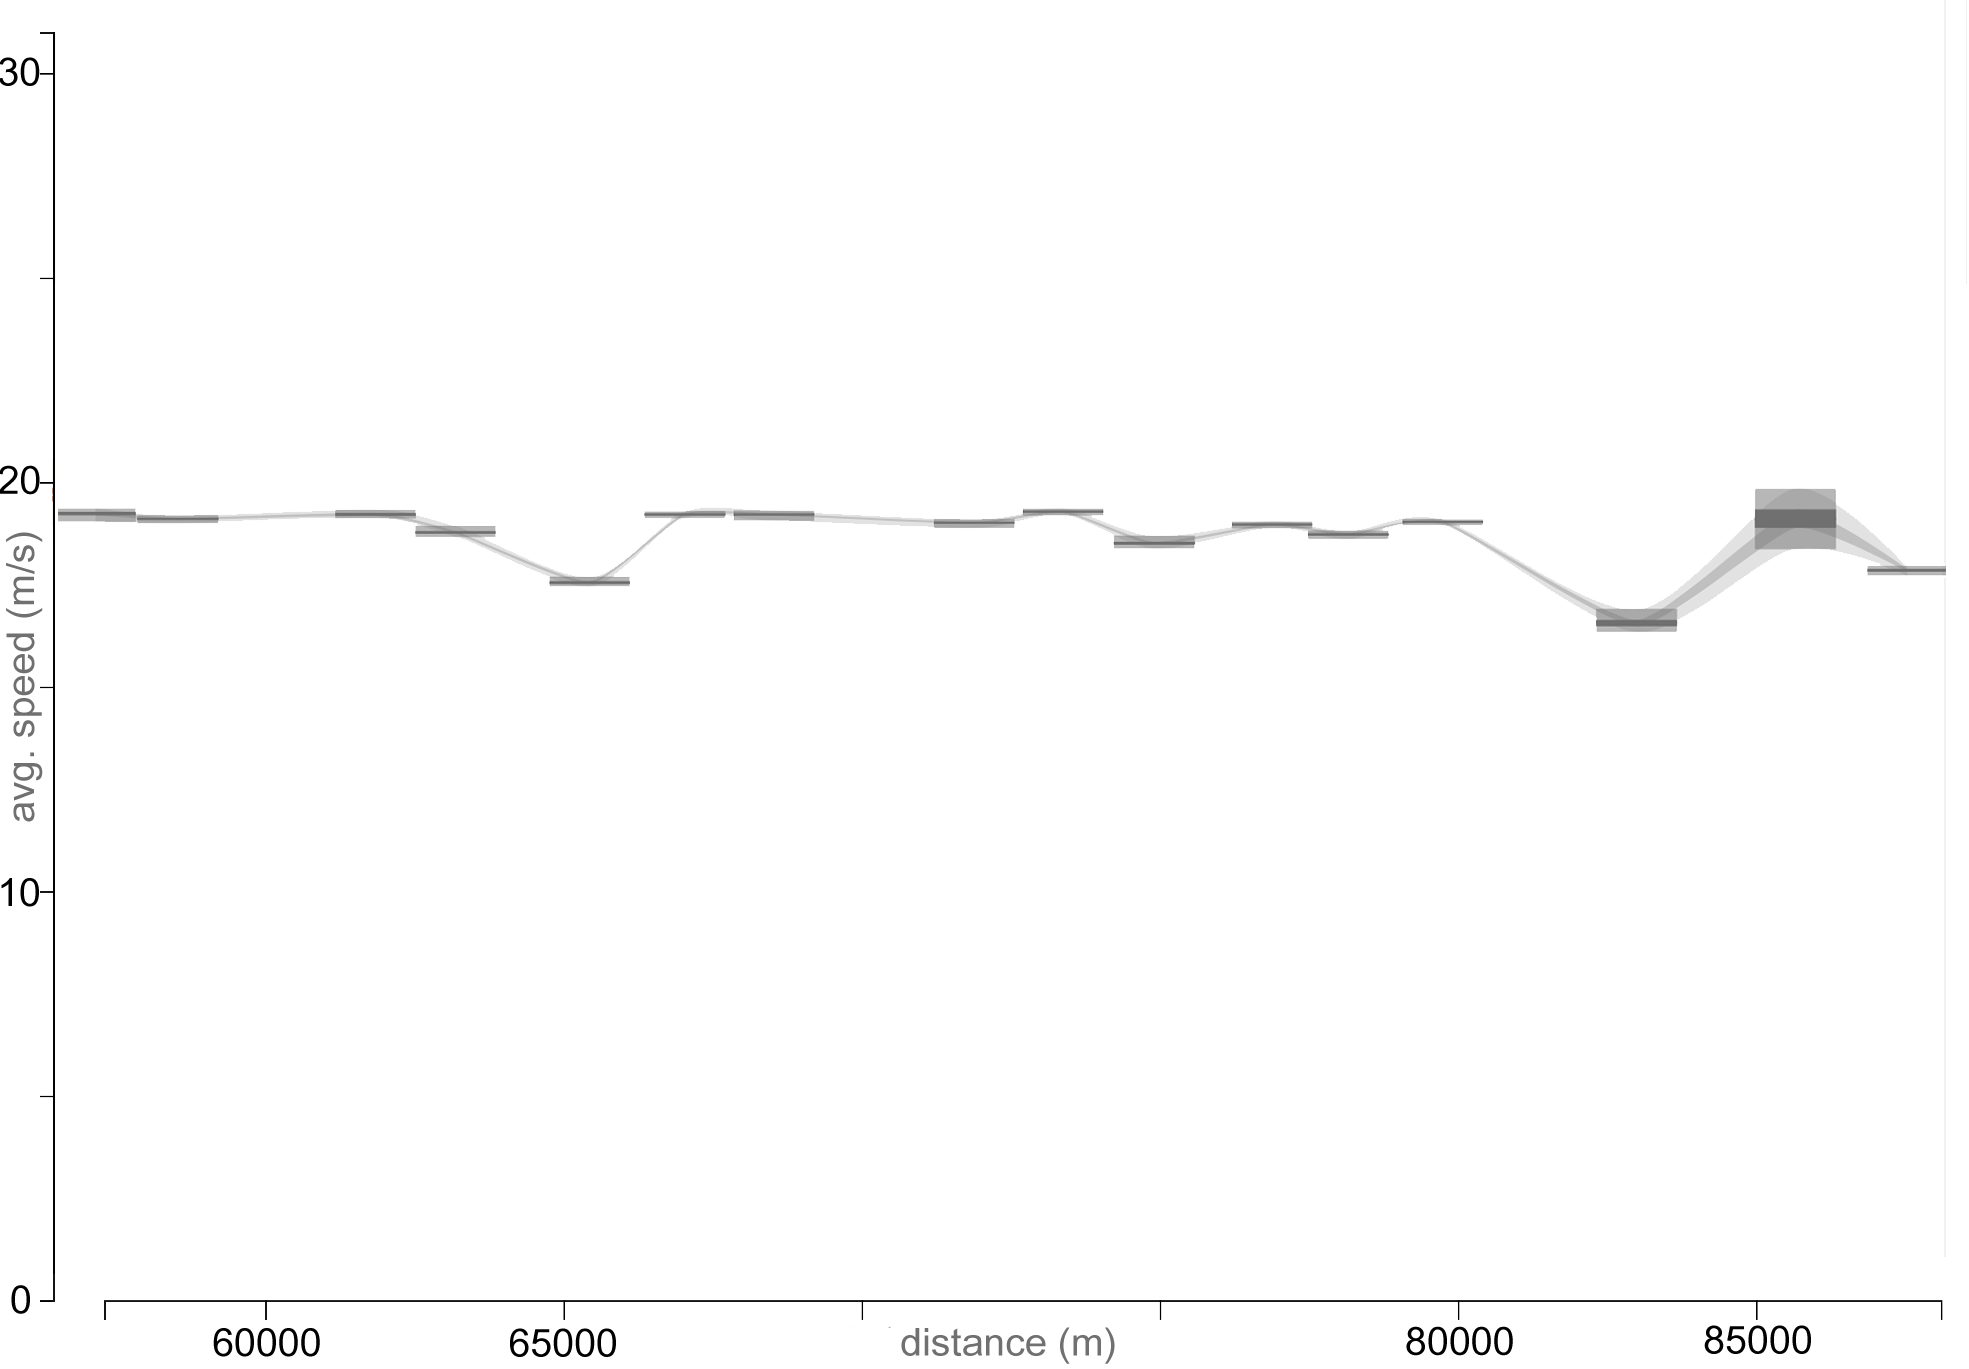
\includegraphics[width=\textwidth]{images/sampling/timestep_a_truth.png}
        \caption{Time window 1.}
        \label{fig:d}
    \end{subfigure}
    \begin{subfigure}{0.32\textwidth}
        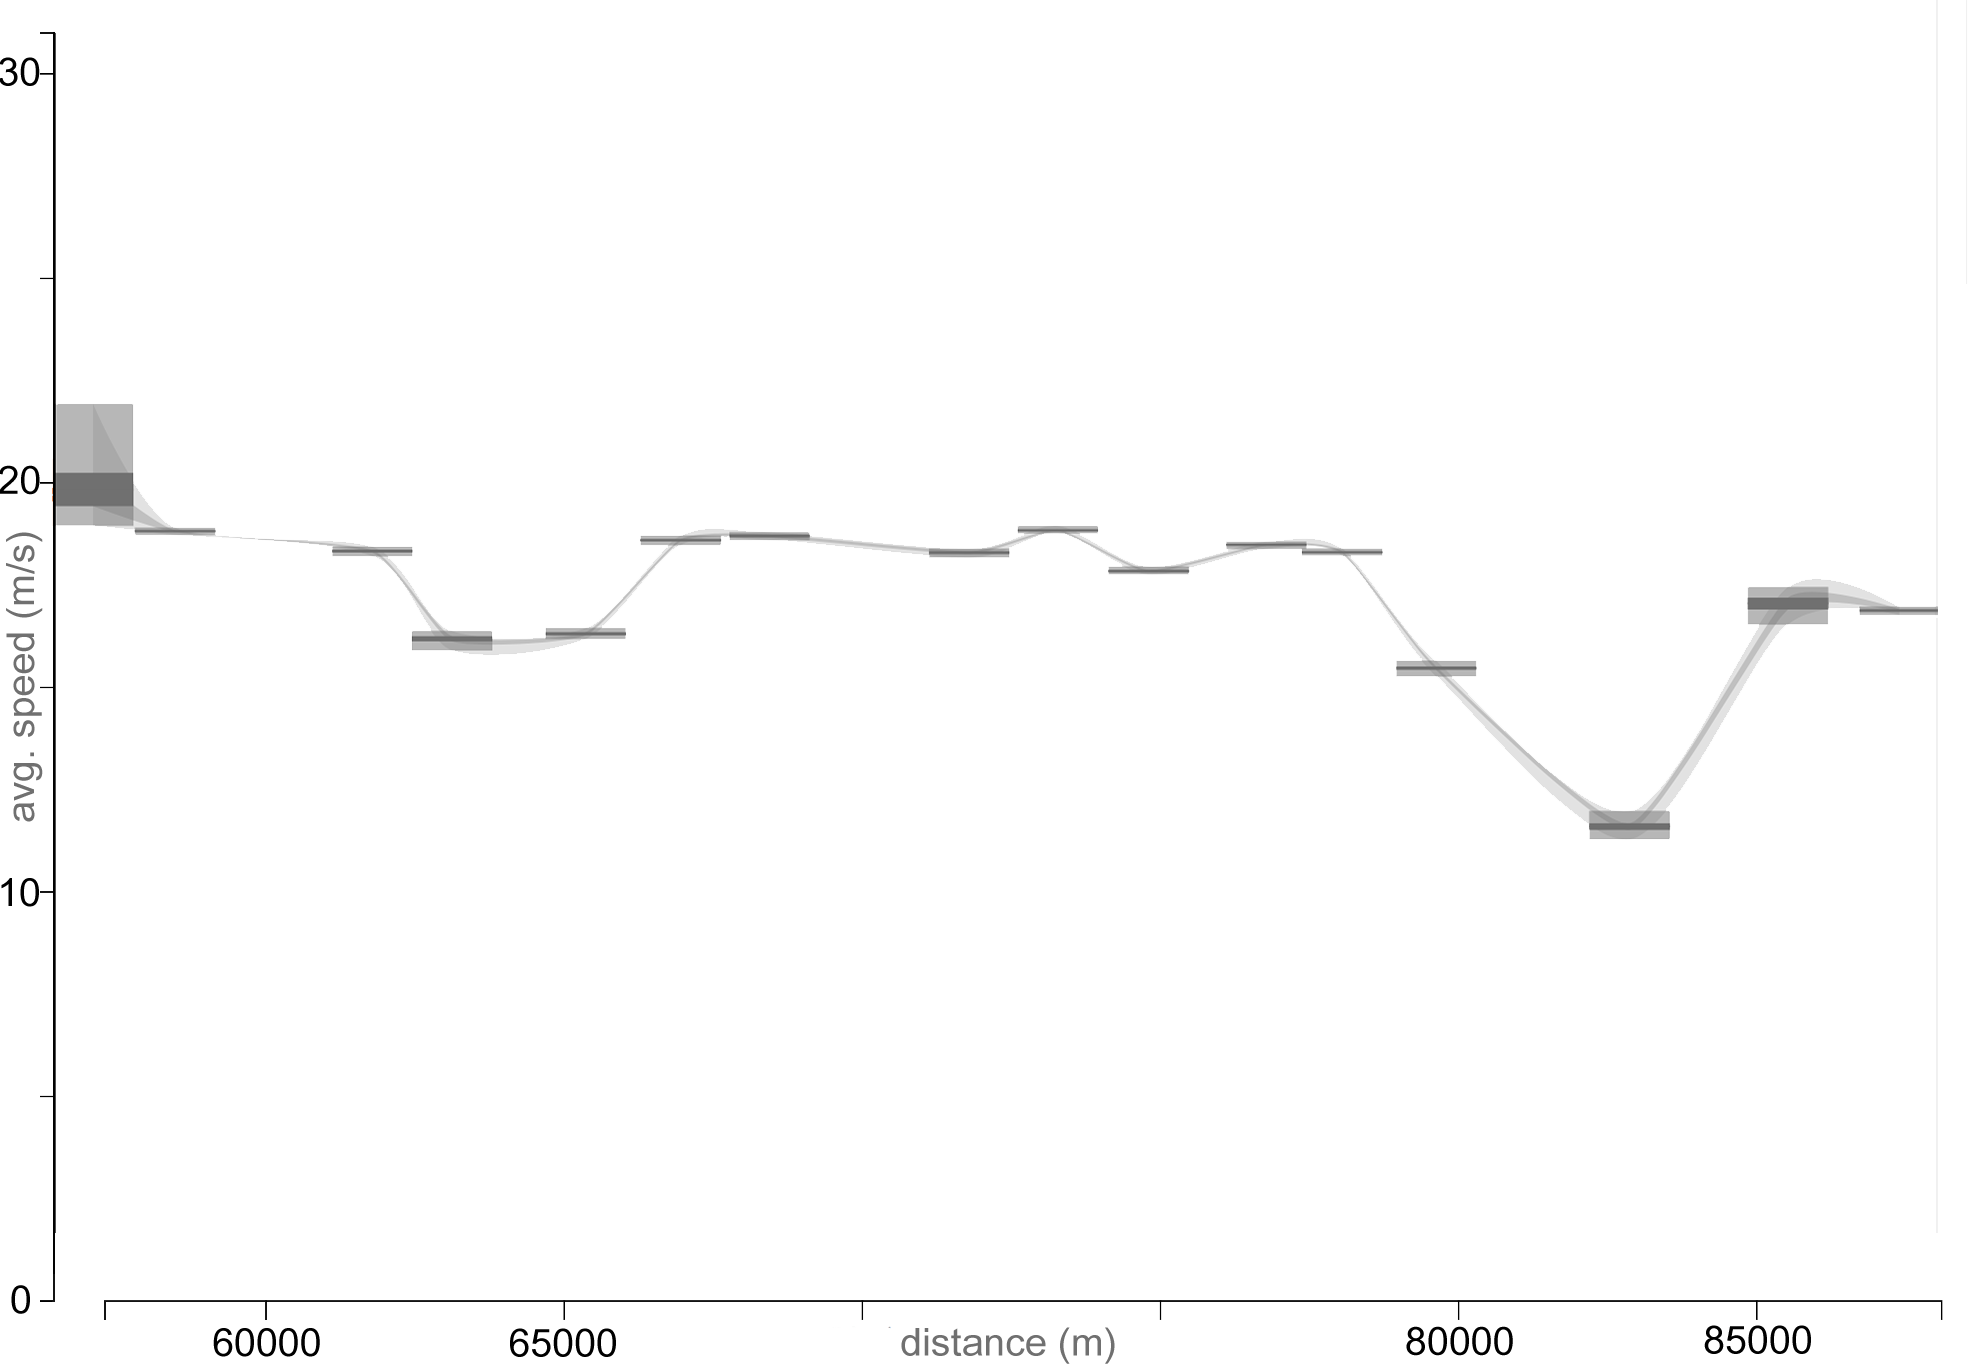
\includegraphics[width=\textwidth]{images/sampling/timestep_b_truth.png}
        \caption{Time window 2.}
        \label{fig:e}
    \end{subfigure}
    \begin{subfigure}{0.32\textwidth}
        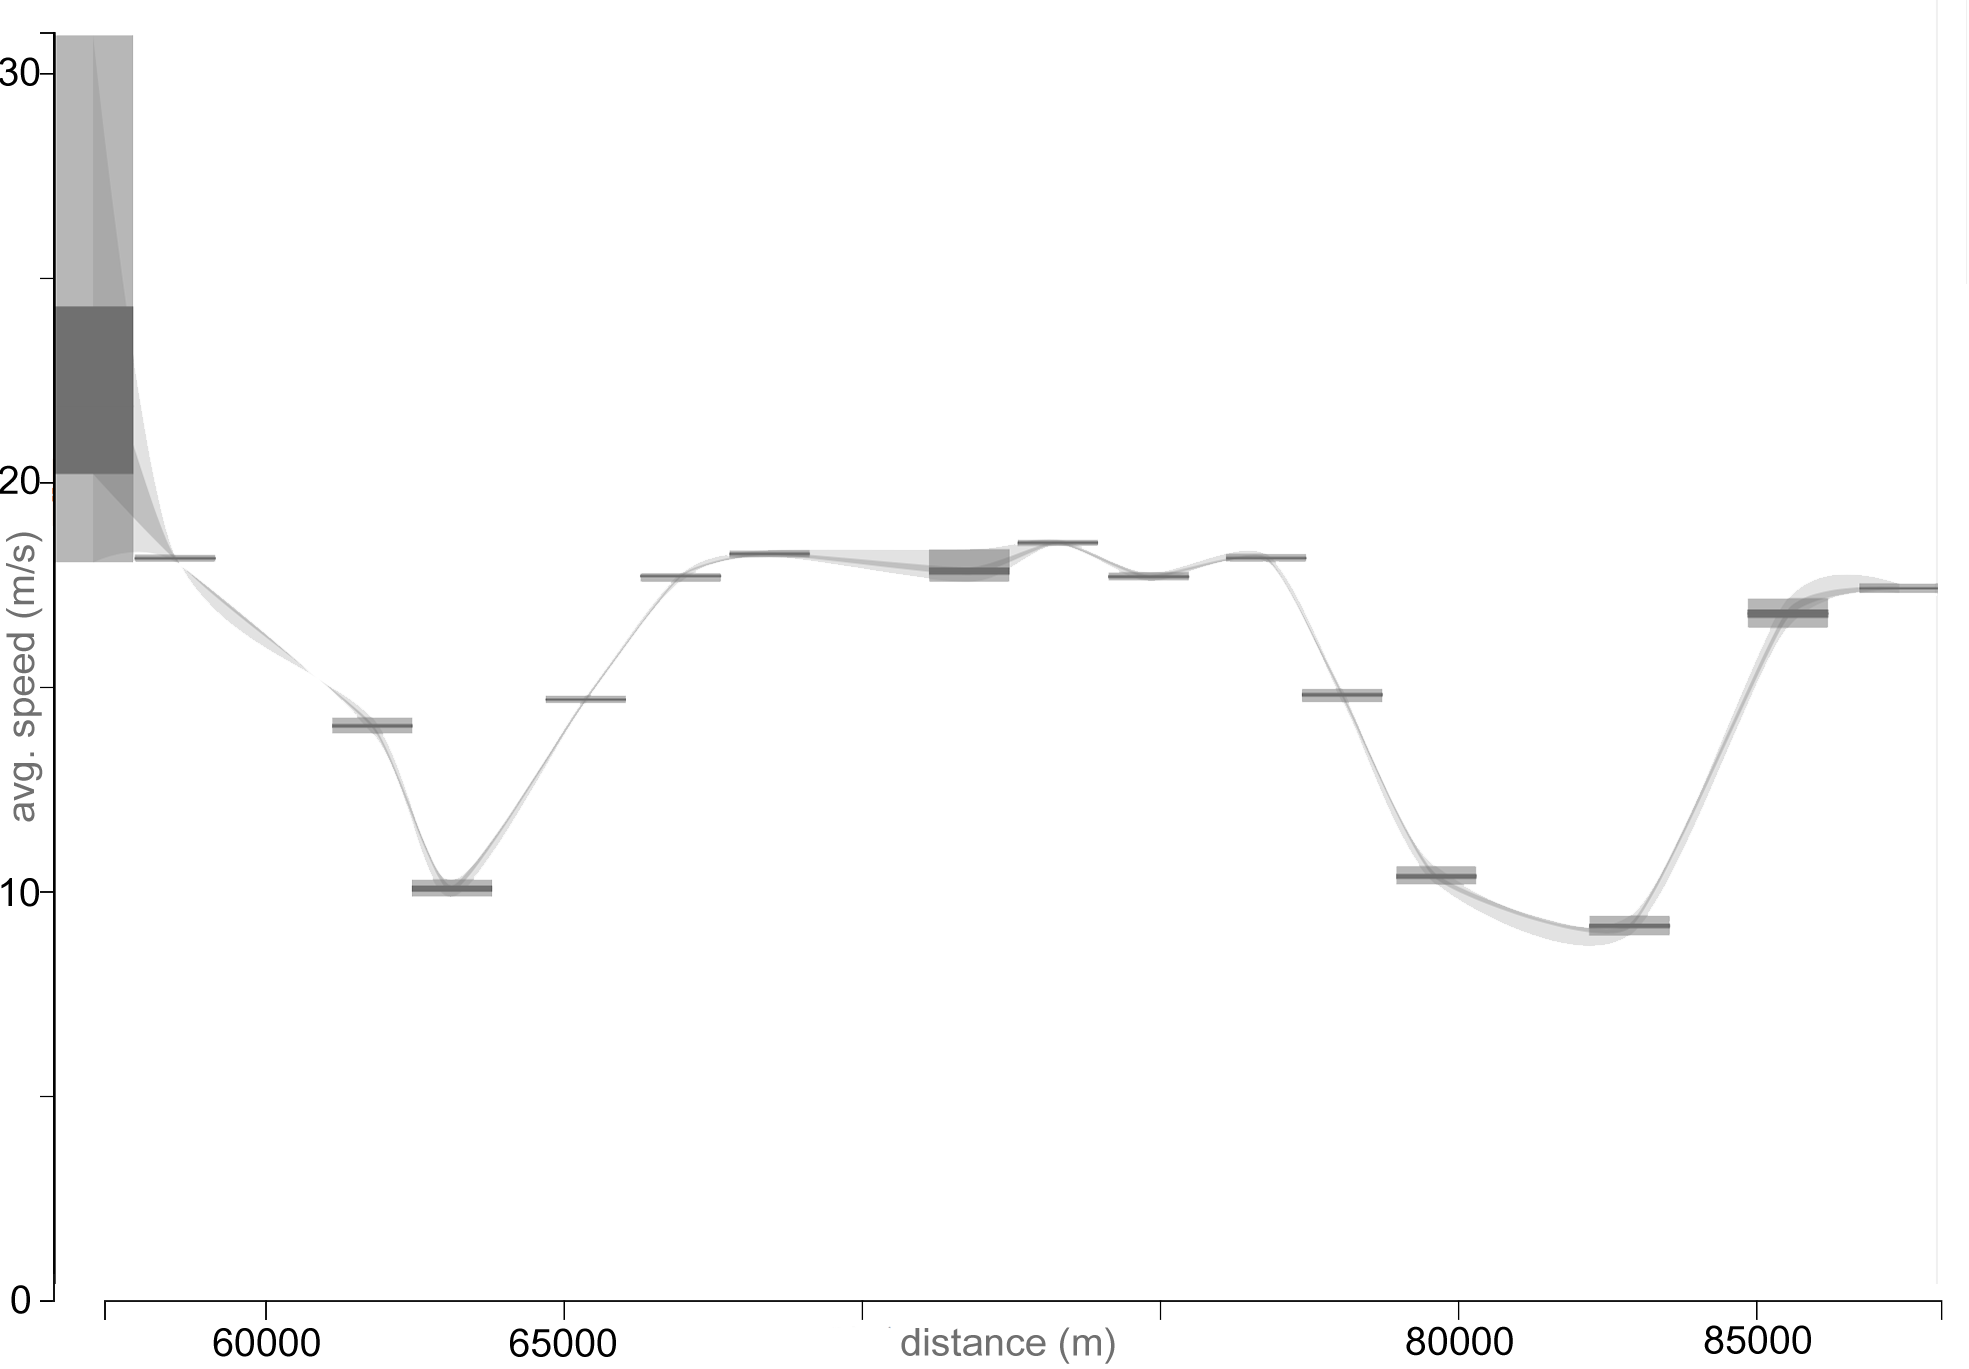
\includegraphics[width=\textwidth]{images/sampling/timestep_c_ground_truth.png}
        \caption{Time window 3.}
        \label{fig:f}
    \end{subfigure}
     \caption{The ``true'' variance in speed for the above scenario, calculated by bootstrapping over the full dataset for each time window.}
     \label{traffic}
\end{figure*}

\subsubsection{Analytical Needs}
The researchers confirmed that, in general, they are interested in ``teasing apart the sources of uncertainty,'' which may or may not be feasible. Lacking that information, they may present their results as a range of possible outcomes with associated confidences.

We proposed that our tool could enable both rapid, rougher estimates of uncertainty, as well as the option to further optimize the predictions. Somewhat surprisingly, there was especially strong interest in the first of these capabilities, the rougher, faster estimate.

One researcher specified that the precise optimization would be useful, but less useful than the less precise but more rapid prediction. He elaborated that at one point, there was a push within the climate modeling community to use ``adjoint methods'' (i.e., sensitivity analysis) to measure uncertainty, but they are quite expensive. “For instance, determining model sensitivity to the choice of particular tuning parameters typically requires 3-4 multi-decadal simulations to see the effect. This is generally untenable with limited computational resources.” Therefore, he said, our rapid estimation would be useful. This could allow scientists to determine which areas---time spans, sets of parameters, etc.---to measure more fully.

Another researcher added that ``basic quality checks are always important'' when analyzing simulations. Visualization to enable qualitative checks such as the growth of uncertainty over time would be very useful, because errors are likely to occur somewhere in the simulation or analysis codes, and visualization tools like ours could help perform basic ``sanity checks'' throughout the modeling process.

\begin{table}[h]
\caption {Training times, and sizes of samples used, for each dataset.} \label{speedup_table} 
\centering
\begin{tabular}{ >{\centering\arraybackslash}m{1.6in}  >{\centering\arraybackslash}m{1.5in} >{\centering\arraybackslash}m{1in} >{\centering\arraybackslash}m{0.5in} >{\centering\arraybackslash}m{1in} >{\centering\arraybackslash}m{1in}}
%\toprule[1.5pt]
%NOTE: edit fractions used based on final results.
{\bf Source} & {\bf Fractions Used} & {\bf Full Size} & {\bf Training}\\ 
Illustris (dark matter simulation) & 0.001, 0.002, 0.003, 0.005, 0.01  & 94 million particles & 188 s\\
\midrule
SUMO (traffic simulation) & 0.05, 0.1 & 9 million entries & 88 s\\
\midrule
CMIP5 (climate models) &  0.0001, 0.0002, 0.0005, 0.001, 0.002, 0.005 & $\sim$2GB per model & 110 s\\
%\bottomrule[1.25pt]
\end {tabular}
\end {table}

%(LK:) the precision needed is driven by what particular question you’re asking. he mentioned being more interested in ‘dominant’ sources of uncertainty. what conclusions are you trying to draw? once we understand a more dominant source of uncertainty, a smaller source of uncertainty may then become more interesting.

One of the atmospheric scientists shared his research interests in depth. He is interested in the likelihoods of extreme weather events, such as extreme precipitation, and how parameter choice affects these likelihoods. One needs many, very high-resolution model runs to properly characterize uncertainty, especially to capture unlikely events. He explores a seven-dimensional space of physical parameters, running a large ensemble of models with values that span the parameter space to try to figure out which sets of parameters most reflect reality. This approach is very expensive, and it is difficult to be sure that one is covering a representative sample of the parameter space, especially because results might not have a continuous dependence on a parameter or combination of parameters. 

%(BT: comparing likelihoods in different climate scenarios, e.g. human emissions and no human emissions. observations can be really hard to come by — only have good observational data for the world (with humans!) for last 30-50 years at best, and for the non-human data, have to be more resourceful (e.g. paleoclimatology?), so correctly characterizing the uncertainty in simulations is even more important

%(BT: talked about work that would have a similar workflow to his, with different particular parameters/outcomes being studied; really into the idea of a flexible tool that could accommodate all of tehse things. could use a list of standardized metrics of climate models that’s avaialble.

All of the researchers, whether working with observations or simulations, strongly emphasized the importance of understanding uncertainty as they work with ensembles of model outputs, and referred to the current difficulty of quantifying and comparing model uncertainties. 
They all assess uncertainty resulting from various parameter or input combinations regularly in their research.

%The workflow of assessing uncertainty resulting from various parameter combinations or initial conditions was common to all of the researchers.

\subsubsection{Our Approach}
The researchers we talked to felt confident that our method and visualization tool could provide useful and accurate information: ``the general idea of taking sub-samples...to inform what the uncertainty is of the ensemble, that's a very straightforward approach, which makes sense to me,'' one said. One person was particularly interested in being able to see the trends in all the samples. Several appreciated the idea that someone interacting with the tool would not have to worry about the specifics of the modeling behind-the-scenes.

Another researcher, the one who explores parameter spaces in climate models, was excited by the idea of an interface like ours, that one can plug any data into, adjust as needed, and flexibly see a quick result. He could imagine interactively tuning the parameters and getting a quick idea of how uncertainty varies with various combinations of parameters, showing him which parts of the parameter space to explore further; this could save a lot of time. We discussed the need for flexibility of data formats and parameter types; he felt it was reasonable for a tool to require a little bit of custom scripting for a particular use case. He pointed us to a standardized list of climate model measures, which could be built into our tool.

\subsection{Case Studies}
\label{results}
For each application---the SUMO traffic model; the Illustris dark matter simulation; the ensemble of CMIP5 ocean models---we show an example use of our method and visualization tool, and discuss successes and difficulties that are particular to each. To interpret the figures: in a boxplot representation, a smaller range indicates higher confidence, and the most likely outcomes are within the darker segments. Throughout this section, ``ground truth'' refers to the uncertainty measured by bootstrapping the full datasets until the results converge. Though we use the ground truth for validation, in a real-world scenario, we expect that users do not have access to the result of this time-consuming calculation.

\subsubsection{Case Study 1: Dark Matter Halos}
We demonstrate our method on halo mass functions in Figure~\ref{hmf_predicted}. In this case,  the halo masses scale with the size of the sample. Therefore, both the magnitudes and the relative values of the uncertainties are strongly dependent on sample size, and both relationships must be described in the model. Our results show a prediction of uncertainty that smoothly decreases with each mass bin, which is the behavior that the ground truth variance converges to.

The magnitude of variance in our prediction roughly matches the ground truth measurement. The predicted variance is on the order of $10^{-4} \mathrm{Mpc}^{-3}$, while the halo mass function peak is about $0.3\mathrm{Mpc}^{-3}$; this is within the desired precision of 1-5 percent~\cite{behroozi},~\cite{tinker}. 

A researcher could use a trained model to quickly check new simulation runs and determine whether the particle shot noise is likely to be within an acceptable level. In the case depicted in Figure~\ref{hmf_predicted}, he would decide that the simulation could proceed because the uncertainty meets the requirements for comparing simulation output to observed data. However, if the particle noise were projected to be too large, he could choose to stop this simulation run and investigate the problem before using more computing resources.

\subsubsection{Case Study 2: Traffic Jam Evolution}
We tested our approach on three consecutive time windows of the traffic model SUMO~\cite{SUMO2012} (see Section~\ref{traffic_sims}). Within each time window, we display the average speed of cars that pass several detectors, measured with two small samples of the simulation data. We simultaneously show the predicted uncertainty values (Figure~\ref{traffic_predicted}), and compare with our calculation of the ``true'' uncertainty (Figure~\ref{traffic}).  

In time window 1 (Figure~\ref{fig:d}), cars travel at a fairly consistent speed, with one slow-down around $x_a = 65,000$ and another, more significant, slow-down around $x_b = 80,000$. Imagine an emergency manager monitoring an evacuation route represented by this traffic model (Section~\ref{traffic_sims}). Looking at Figure~\ref{traffic}, she sees a confident prediction that the jam at $x_a$ will be alleviated after a short distance. 

Meanwhile, the emergency manager can see that for the jam at $x_b$, there is a much more significant probability that the jam will get worse through $x=83,000$m. Therefore, she focuses on this second jam location to look for alternate routes there. Indeed, in Figure 7 we see with high confidence that the second jam continues to worsen.

In general, our model overestimates the magnitude of the variance. Since the training samples display more variance in average speed (because outliers have a stronger influence over the average of smaller samples), this extra variance is reflected in our prediction. To mitigate this effect, one could include more samples; then, the model would have more training to recognize a diminishing variance with larger sample sizes. We see this in Figure~\ref{traffic_predicted}, where larger samples (orange) have slightly lower variance than smaller samples (green).

\label{ohc_case_study}
\begin{figure*}[h]
    \centering
    \begin{subfigure}{0.49\textwidth}
        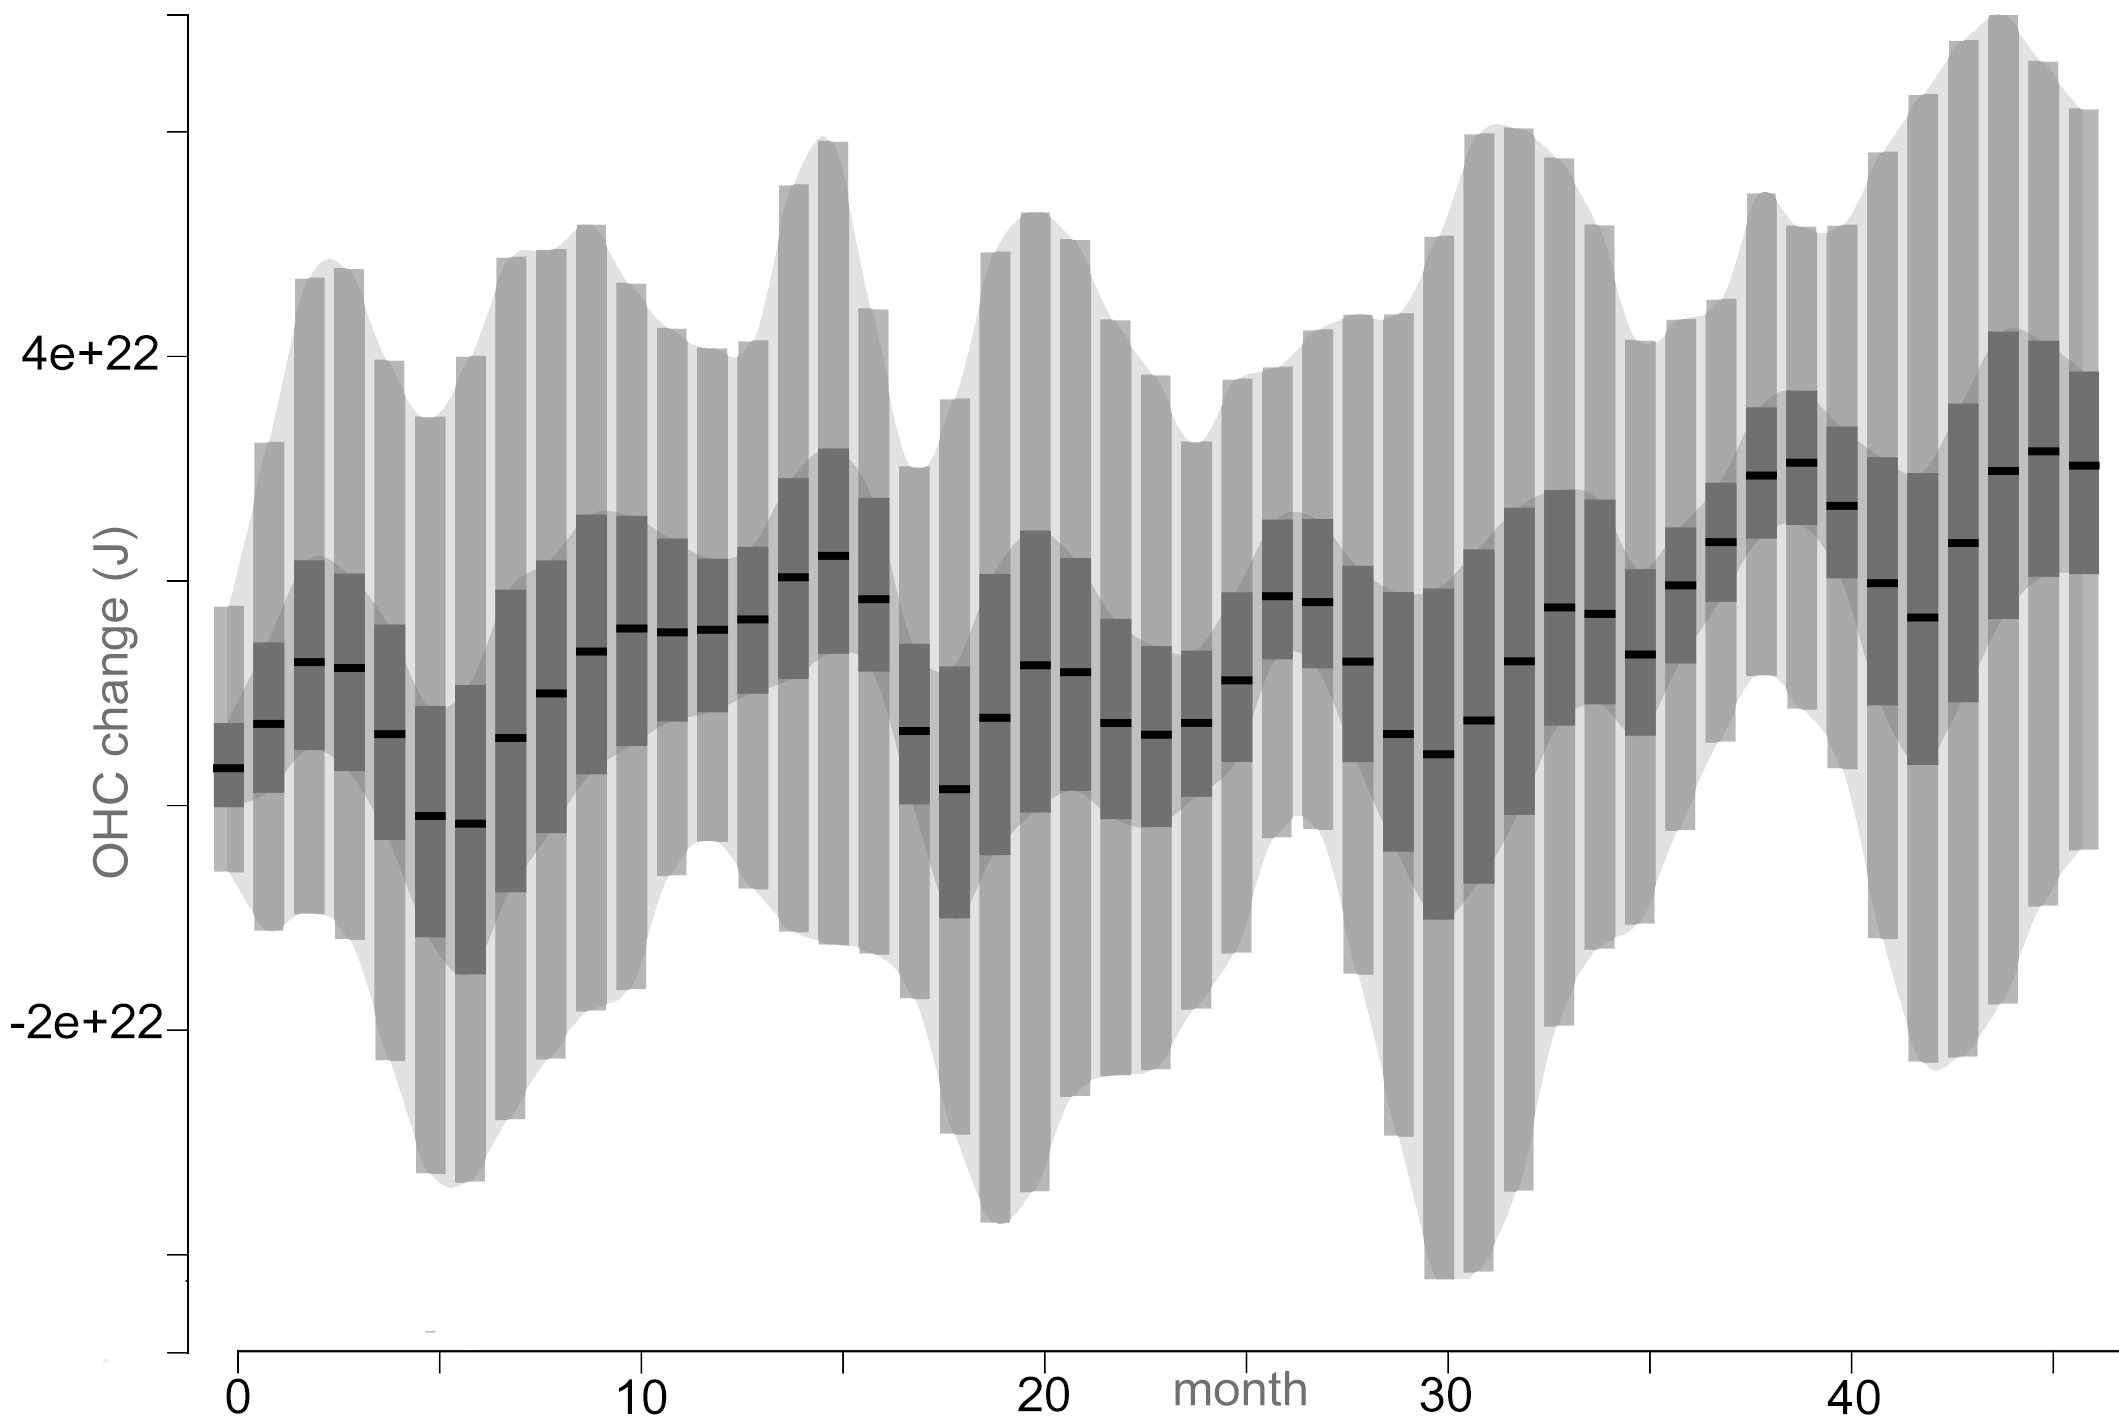
\includegraphics[width=\textwidth]{images/sampling/cmip_prediction_2006_2010_cropped.png}
        \caption{Predicted variance in ocean heat content change, 2006-2009.}
        \label{ohc_predicted_a}
    \end{subfigure}
    \begin{subfigure}{0.49\textwidth}
        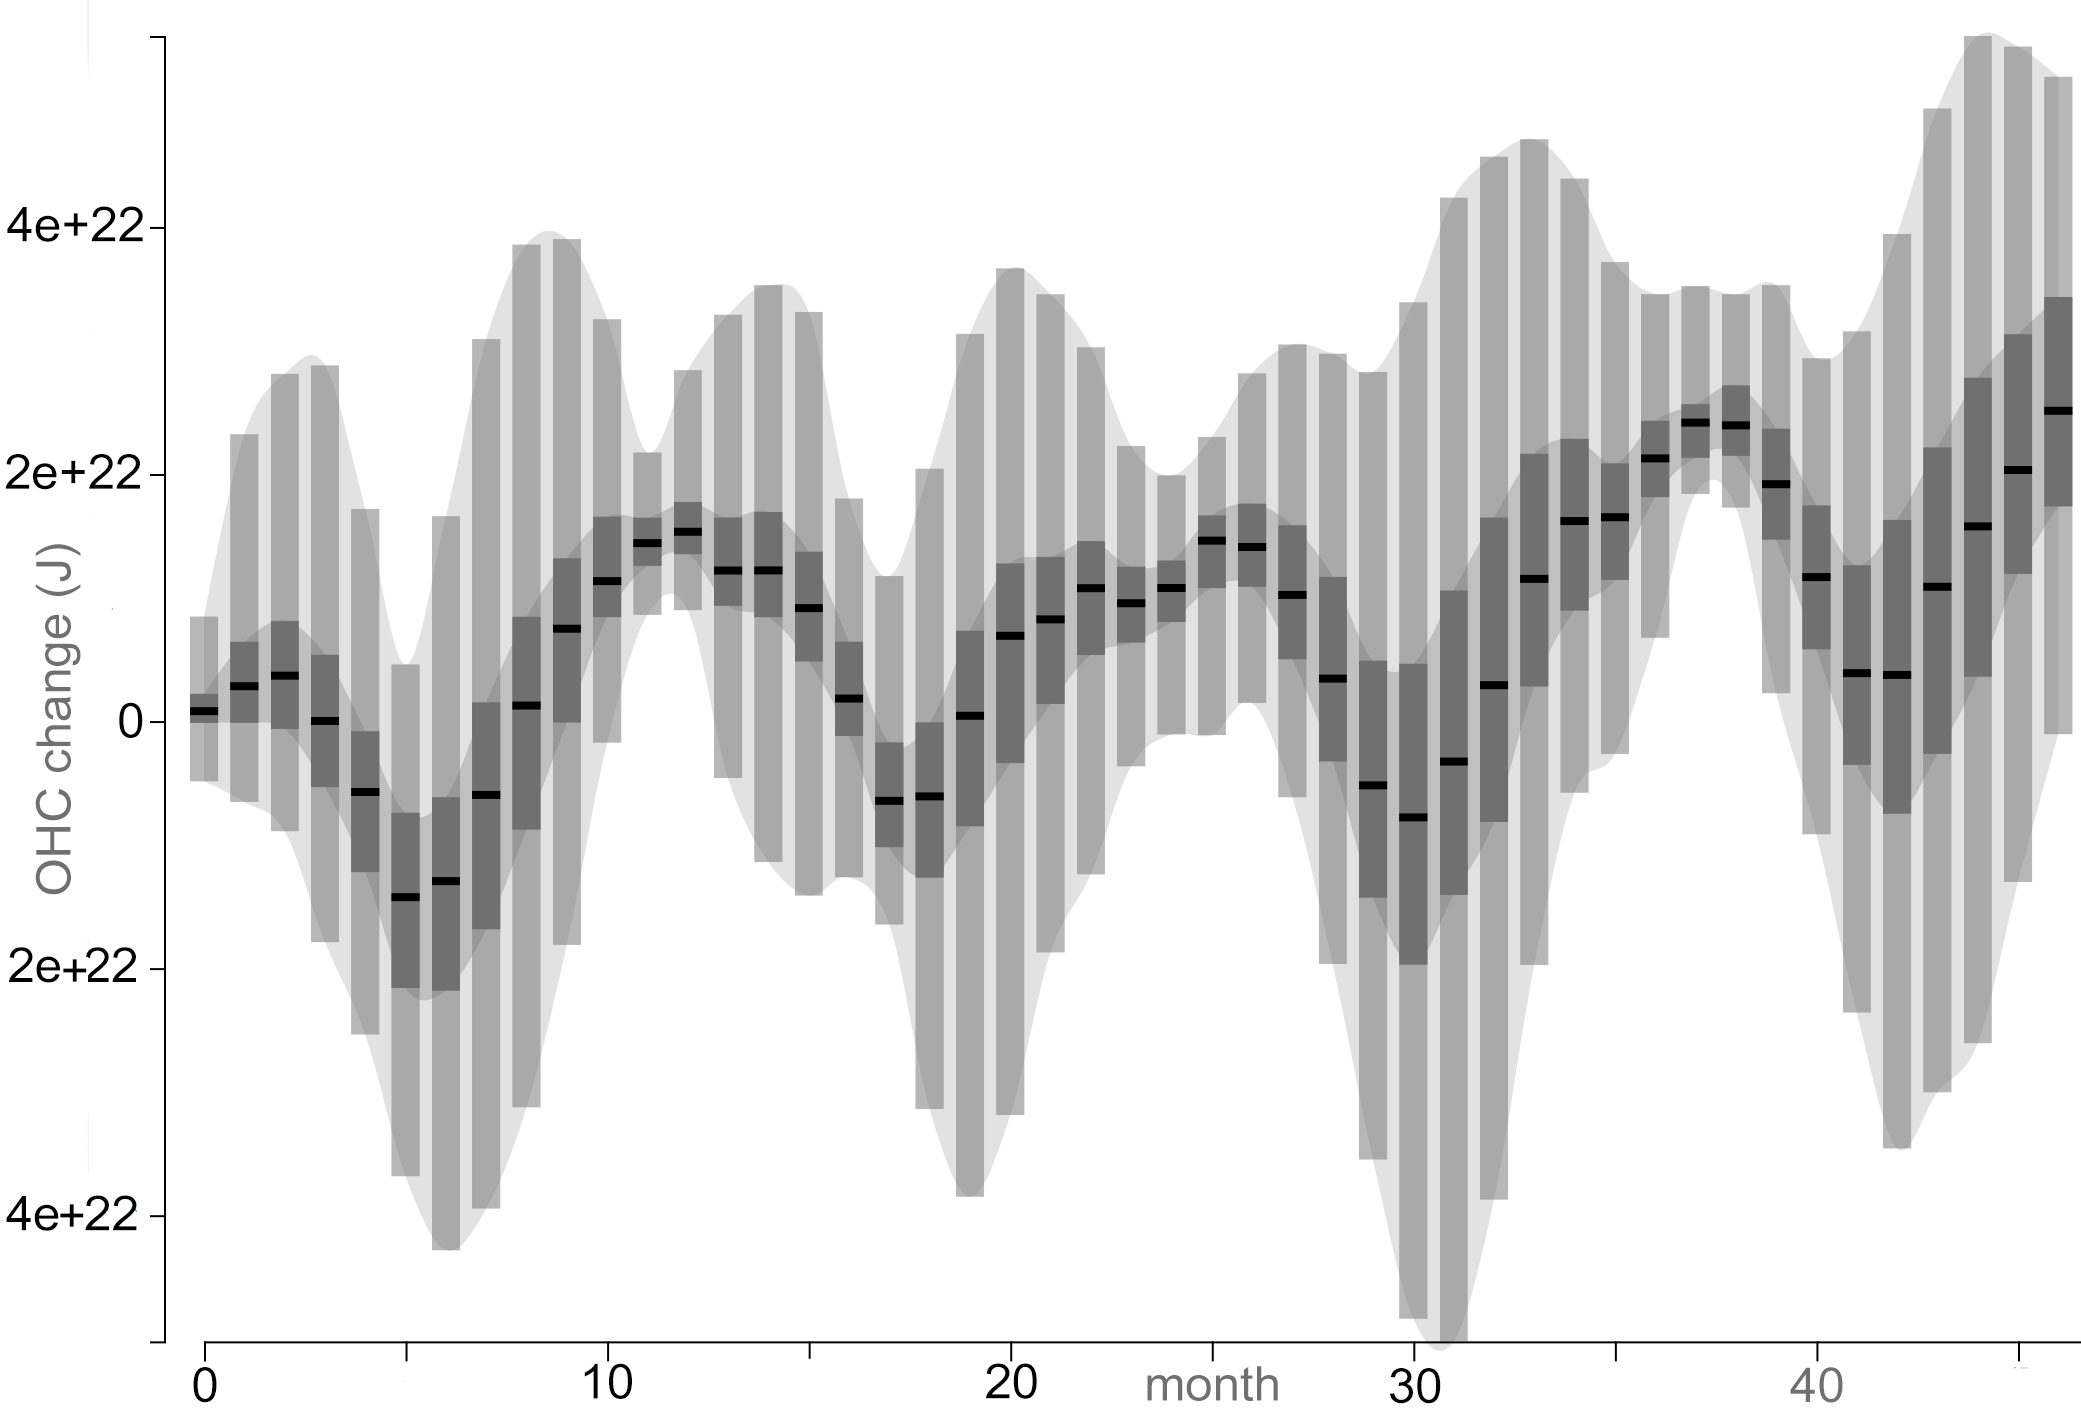
\includegraphics[width=\textwidth]{images/sampling/cmip_ground_truth_2006_2010.png}
        \caption{``True'' variance in ocean heat content change, 2006-2009.}
        \label{ohc_true_a}
    \end{subfigure}
     \caption{CMIP5 ensemble data from 2006-2009.}
     \label{ohc_a}
\end{figure*}

\begin{figure*}[h]
    \centering
    \begin{subfigure}{0.49\textwidth}
         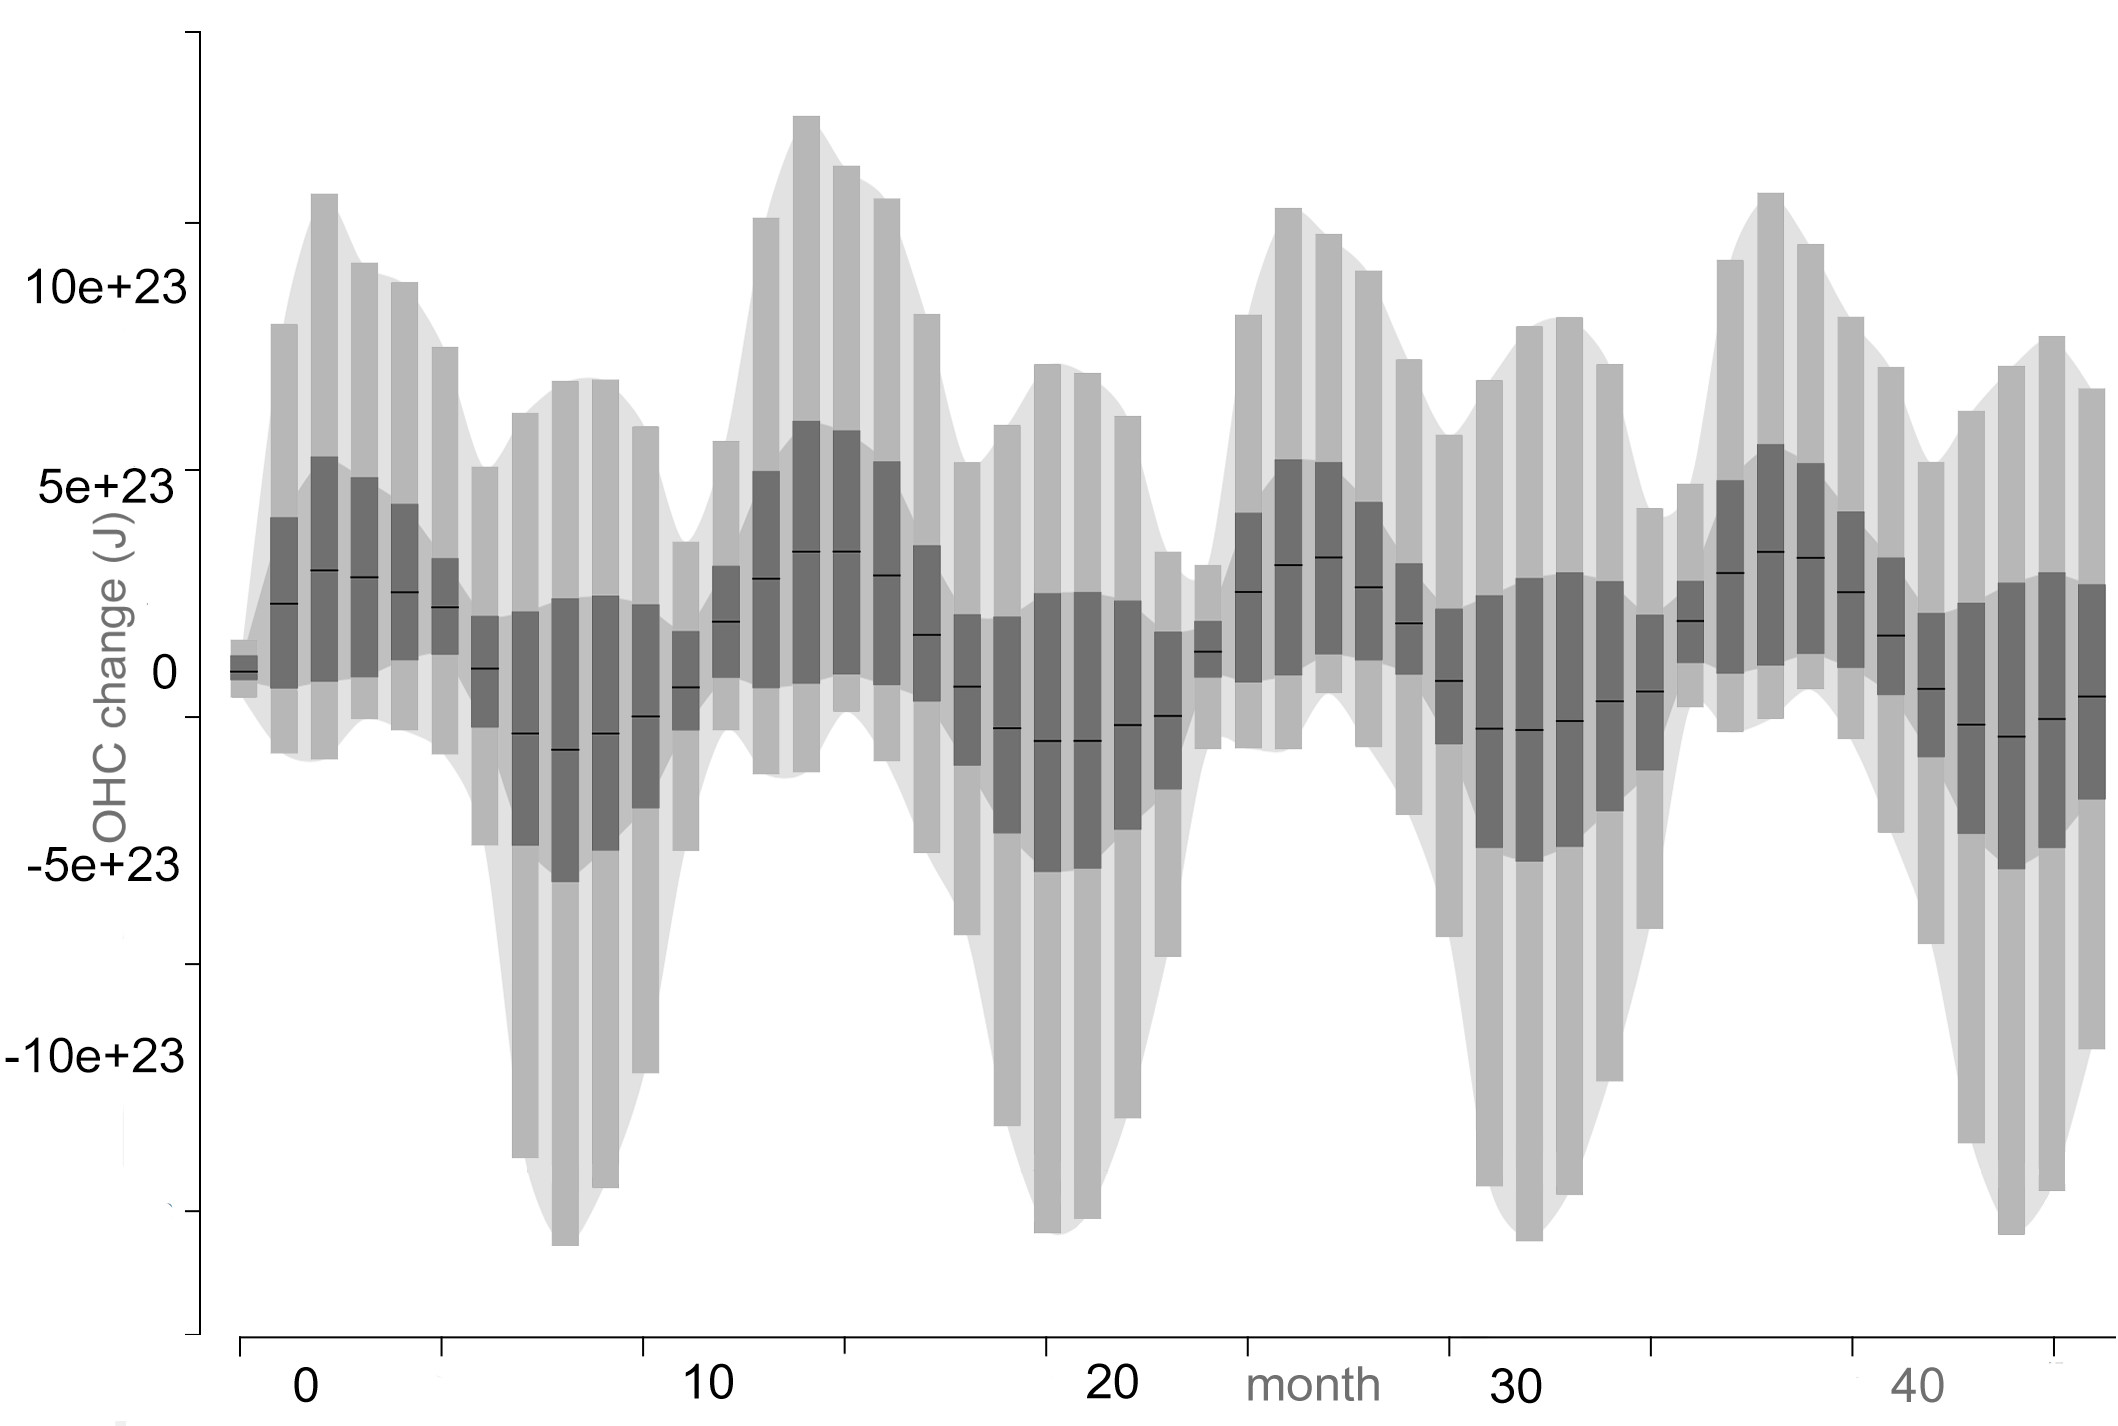
\includegraphics[width=\textwidth]{images/sampling/2010_2014_predictions}
        \caption{Variance in ocean heat content change, predicted with the model trained above (Figure~\ref{ohc_predicted_a}), 2010-2013.}
        \label{ohc_predicted_b}
    \end{subfigure}
    \begin{subfigure}{0.49\textwidth}
        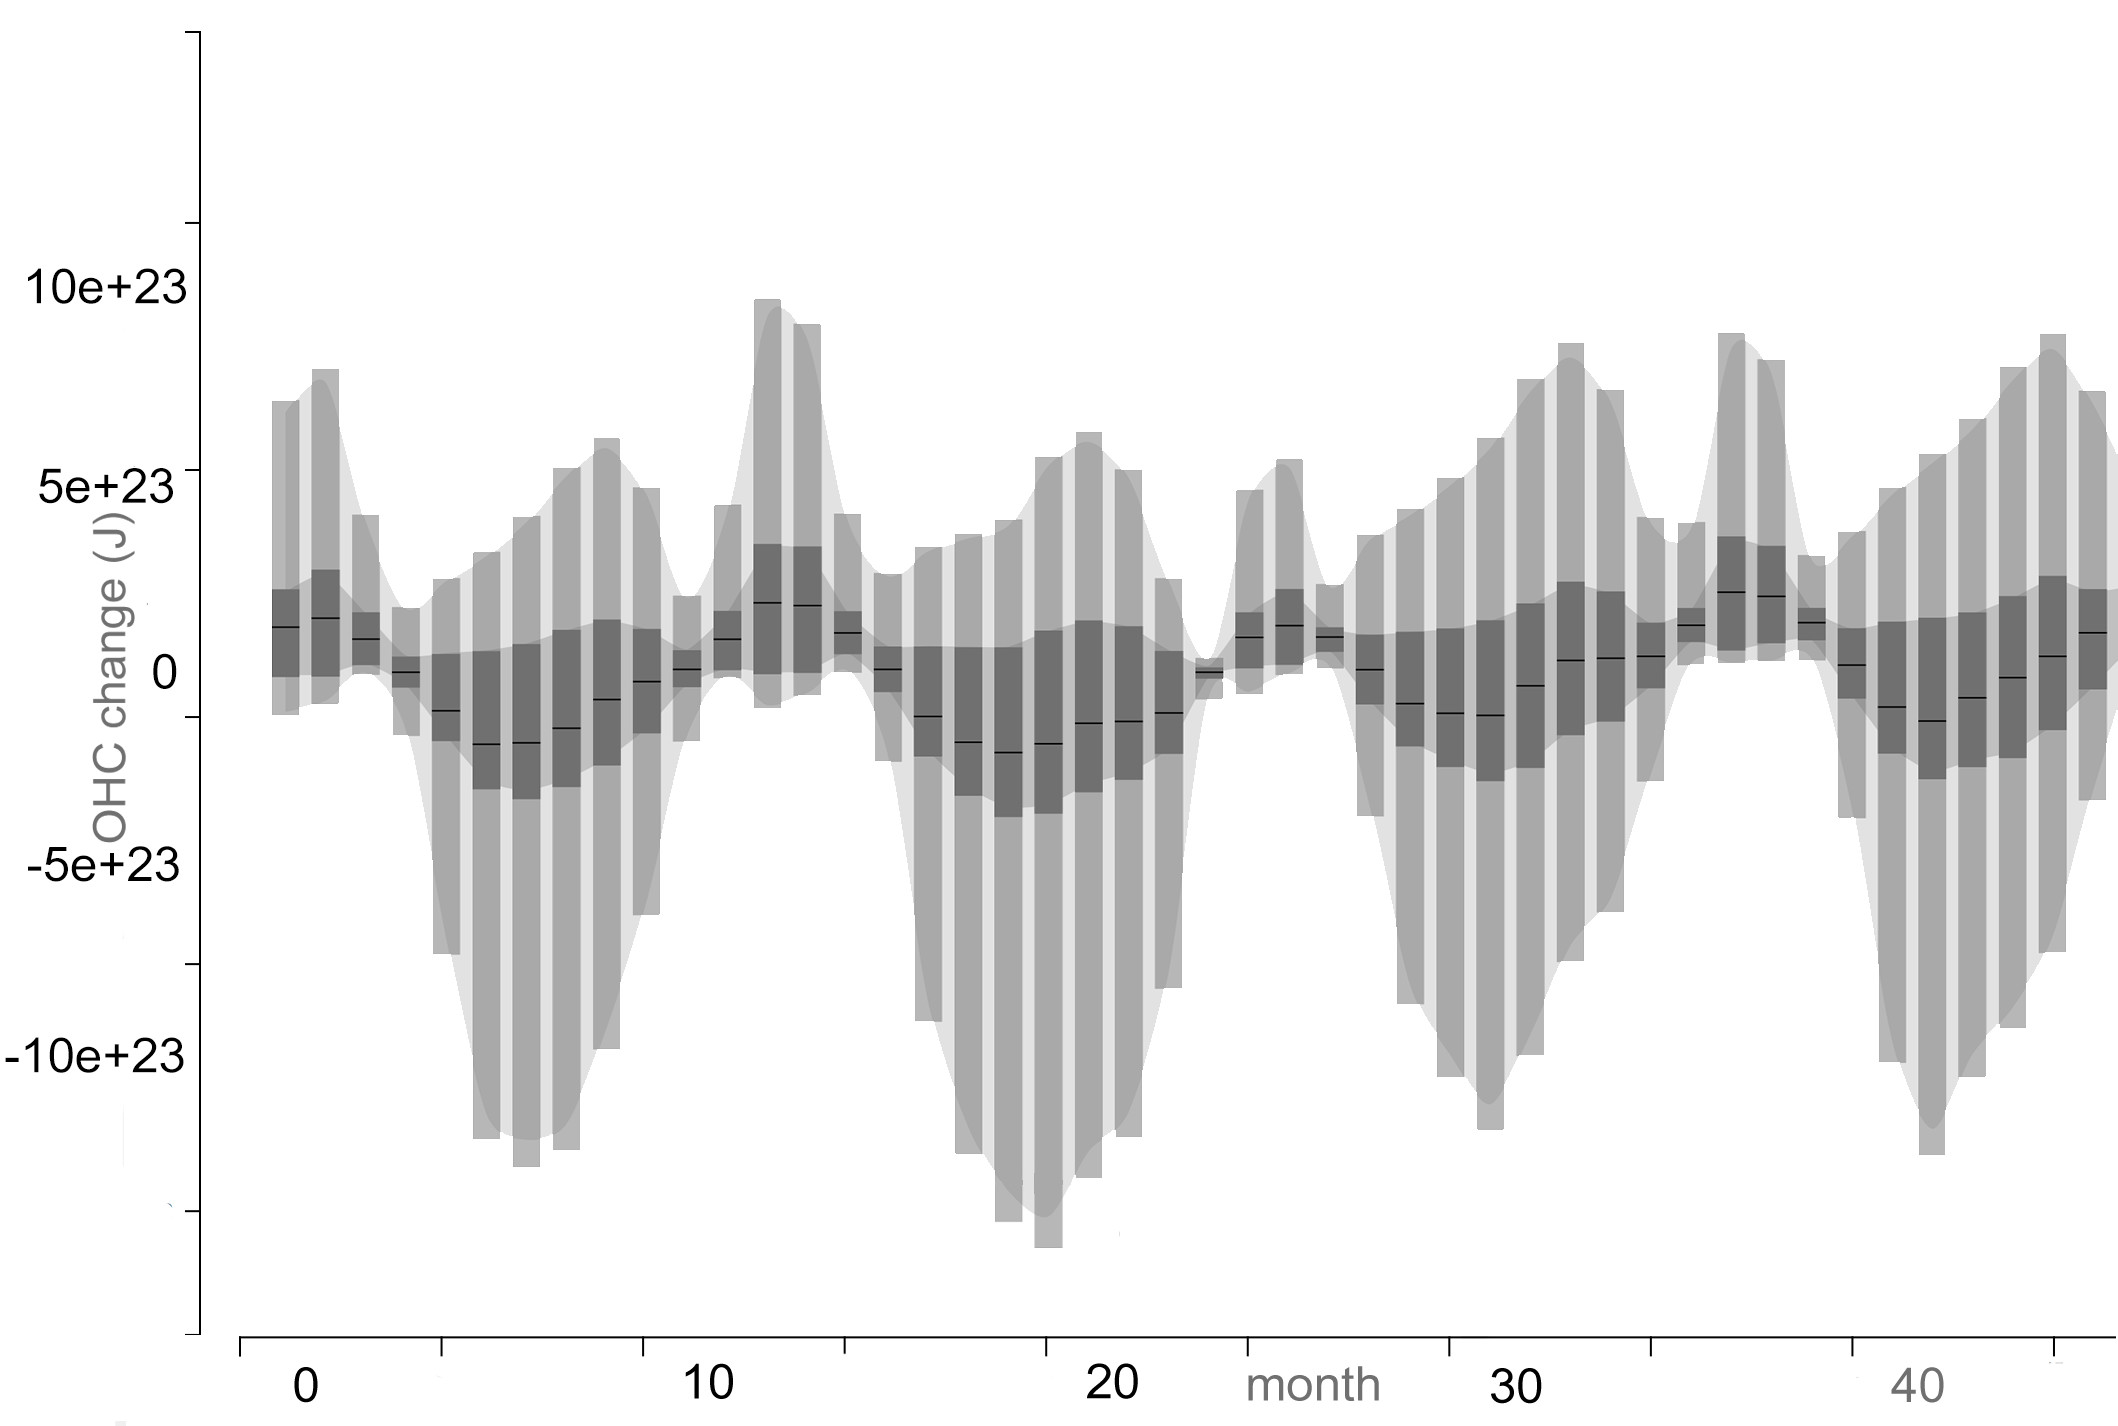
\includegraphics[width=\textwidth]{images/sampling/cmip_truth_2010-2014}
        \caption{True variance in ocean heat content change, 2010-2013.}
        \label{ohc_true_b}
    \end{subfigure}
     \caption{CMIP5 ensemble data from 2010-2013 (a different combination of models than those used in training), the testing dataset.}
     \label{ohc_b}
\end{figure*}

\subsubsection{Case Study 3: Rising Ocean Heat Content}
As described in Section~\ref{climate_models}, we sampled an ensemble of ocean models, then performed our bootstrapping method over the ensemble to measure uncertainty. Our set of models is smaller than ensembles that researchers may use in practice, so our results are noisier than real-world results might be. The shape of the uncertainty contours is largely accurate: almost all of the values have the correct relationships with neighboring values, and the periodic increase is reflected. However, our model (Figures~\ref{ohc_predicted_a},~\ref{ohc_predicted_b}) overestimates the magnitude of the variance (Figures~\ref{ohc_true_a},~\ref{ohc_true_b}). In general, scientists are interested in constraining uncertainty; overestimation can still be useful. 

Many scientists are primarily interested in the relative confidence levels for different sets of parameters. A researcher could use our prediction to see that, for the set of parameters used in our example, the magnitude of uncertainty tends to increase at later times, and that the peak OHC values (e.g. month 26, month 38) have higher confidence than the lower values. Then, the researcher could feed another dataset to the model, such as a sample from another simulation with different input parameters or initial conditions, to see how this difference affects the confidence in the OHC values. We tested this workflow by applying our trained model to OHC values from another ensemble of CMIP5 simulations for a different time period, 2010-2013 (see Figure~\ref{ohc_predicted_b}). The prediction shows a higher likelihood of greater seasonal swings in OHC than in the years 2006-2009. This increasingly volatile behavior is confirmed in Figure~\ref{ohc_true_b}.
	
The most accurate results we obtained for this case study omitted the three smallest sample sizes we had taken (see Table~\ref{speedup_table}). Comparing uncertainties for these samples in the interface, we could see that the smallest samples did not have a consistent pattern. Omitting these samples, we got a better prediction result; this is an example of how human-guided reasoning with our tool is a helpful supplement to modeling.
    %note: if/when i present about this, this would be a good example slide

% this phenomenon is something to watch out for when the measurement is an average (?). (Similar to climate.)

%explain the other outliers.

%quantitative results here.

\subsubsection{Performance}
%Results go here.
Compared to calculating uncertainty with bootstrapping on a full dataset, our method offers a speedup of $\mathcal{O}(N)$ (where $N$ represents the sample sizes used). That is, for each of our case studies, the relationship between sample size and uncertainty computation time is roughly linear. Note that, for the dark matter data, our speedup is highly dependent on halo finder implementation; some halo finders can be parallelized for efficient performance, though halo finding in general is quite expensive.

We also report model training times in MATLAB for each of the applications. These times were measured on an iMac with a 4GHz processor. Our aim is to show our method's feasibility with easily accessible computing resources. These times reflect the results shown in the case study images, but more precise results are usually possible with more fitting iterations and/or more hyperparameters.

% SHOW SCALABILITY.
%\caption {Training time for the regression model in each case study.}
%\label{speedup_table}

\subsection{Limitations}
%Lower limit on sample sizes.
For each application, there is a lower limit on the possible sample sizes. One reason is that a sufficiently small sample size captures too little information to provide to a model; these very small samples may omit large groups of outliers and/or be overly influenced by the inclusion of outliers (see section~\ref{traffic_case_study}). It should be possible, however, to identify these cases using our tool. If sampled uncertainties do not follow any discernible pattern, they are likely too subject to noise and therefore too small to use for modeling. With an increased simulation size, one can attain equally good results with smaller relative fractions; however, too extreme a discrepancy between sample size and absolute size makes extrapolation difficult.

% unsure whether this would work on all simulation types! e.g. astrophysical ones. depends on type of data and type of measurement, probably. future work can come up with more concrete limitations.

%scaling / log ...

% wrap up with summary of what works & what doesn't for each application we tested.
% - HMF was very hard because of the scaling; also, there are some pretty scalable halo finding algorithms out there, so it's harder for us to claim a significant improvement
% - OHC was easier, but ...
% - traffic ?

\section{Conclusion and Future Work}
Our method and visualization tool can facilitate fast estimates of discreteness uncertainty in several types of simulations. We establish that our method is generally transferable to researchers who need to characterize uncertainty in their simulations. However, in this study, we limit our tests to one category of uncertainty, which we measure with one type of approach. Separating sources of uncertainty is difficult, so our method provides the benefit of understanding one particular source in isolation. In the future, though, more tools need to be created, with capabilities such as sensitivity analysis to separate causes of uncertainty, and offering enhanced ability to supervise prediction kernels.

Methods and tools such as ours can be used as a basis to implement more complex or domain-specific uncertainty quantification. More broadly, tools like ours, which favor generalizability and applicability to realistic scenarios over precision, will be crucial for expanding the next generation of usable scientific visualization tools.
\chapter{Uncertainty-Aware Visual Analysis for Remote Sensing}
\section{Introduction: Wildfires and Emergency Management}
Wildfires are an increasingly frequent source of destruction in many regions, including the western United States, causing billions of dollars in losses in destroyed structures, agriculture, and fire-fighting resources, emitting harmful aerosols into the air (Figure~\ref{teaser}), and triggering evacuations~\cite{Smith2013}. Fires are most often caused by humans, making it difficult to predict where they might be started; they are also highly complex, influenced by factors such as weather, wind speed, vegetation, and terrain, and therefore it is quite difficult to model their spread~\cite{gollner2015towards}. Many types of relevant data are available, for historical fires and/or in real time, from local, state, and federal government agencies. These data include satellite detections, vegetation maps, fire perimeters, loss estimates, written descriptions, and weather station data, among others; additional data, such as soil composition, are relevant to hazards, such as mudslides, which may be triggered several months after a wildfire.

% * <mvgomov@ucdavis.edu> 2018-07-16T21:06:20.686Z:
% 
% > is relevant to events that are triggered by wildfires, such as mudslides.
% I believe the term that Dana used for these is hazards, and it might be worth noting that they're hazards "down the road" (e.g. mudslides might be months later when the rains come), and also preventable if addressed in a timely manner (e.g. re-seeding an identified mudslide hazard); this helps motivate the work just a bit more?
% 
% ^.
These sources of information suffer from a range of uncertainties, including detections affected by smoke or cloud cover, human error, inconsistent information from different people or sensors, incorrect time stamps, and others.
Emergency managers must make decisions about evacuation, fire prevention, and fire mitigation based on these often incomplete, delayed, or otherwise problematic pieces of information. The stages of emergency management decision-making include several assessments that must be made with awareness of probability and uncertainty, including ``identification of increased potential for an event'' and deciding that ``the event is likely or imminent''~\cite{Baumgart2006}. Lacking precise predictions for the movement of a fire---current modeling techniques are not fast or accurate enough to be useful in real time---emergency managers must often use broad characterizations: \textit{which direction is the fire moving, and how fast?}, to make decisions such as whom to notify of evacuation, where to send resources, and what the economic losses might be. 

This project is a result of the early stages of collaboration with local and statewide emergency management organizations, with personnel who are interested in improved data ingestion, display, and analysis capabilities in real time. Currently, emergency managers often use simple visualization tools such as Geographic Information System (GIS) dashboards to explore the types of data outlined above. Improved data analysis and visualization capabilities could be applied to all aspects of emergency management, which include preventing, mitigating, managing, and recovering from disasters~\cite{Akter2017}.
% * <mvgomov@ucdavis.edu> 2018-07-16T21:04:31.120Z:
% 
% > Currently, emergency managers often use simple visualization tools such as GIS dashboards to explore the types of data outlined above.
% You should explain what GIS is before you use the term
% 
% ^.
\begin{figure*}[t]      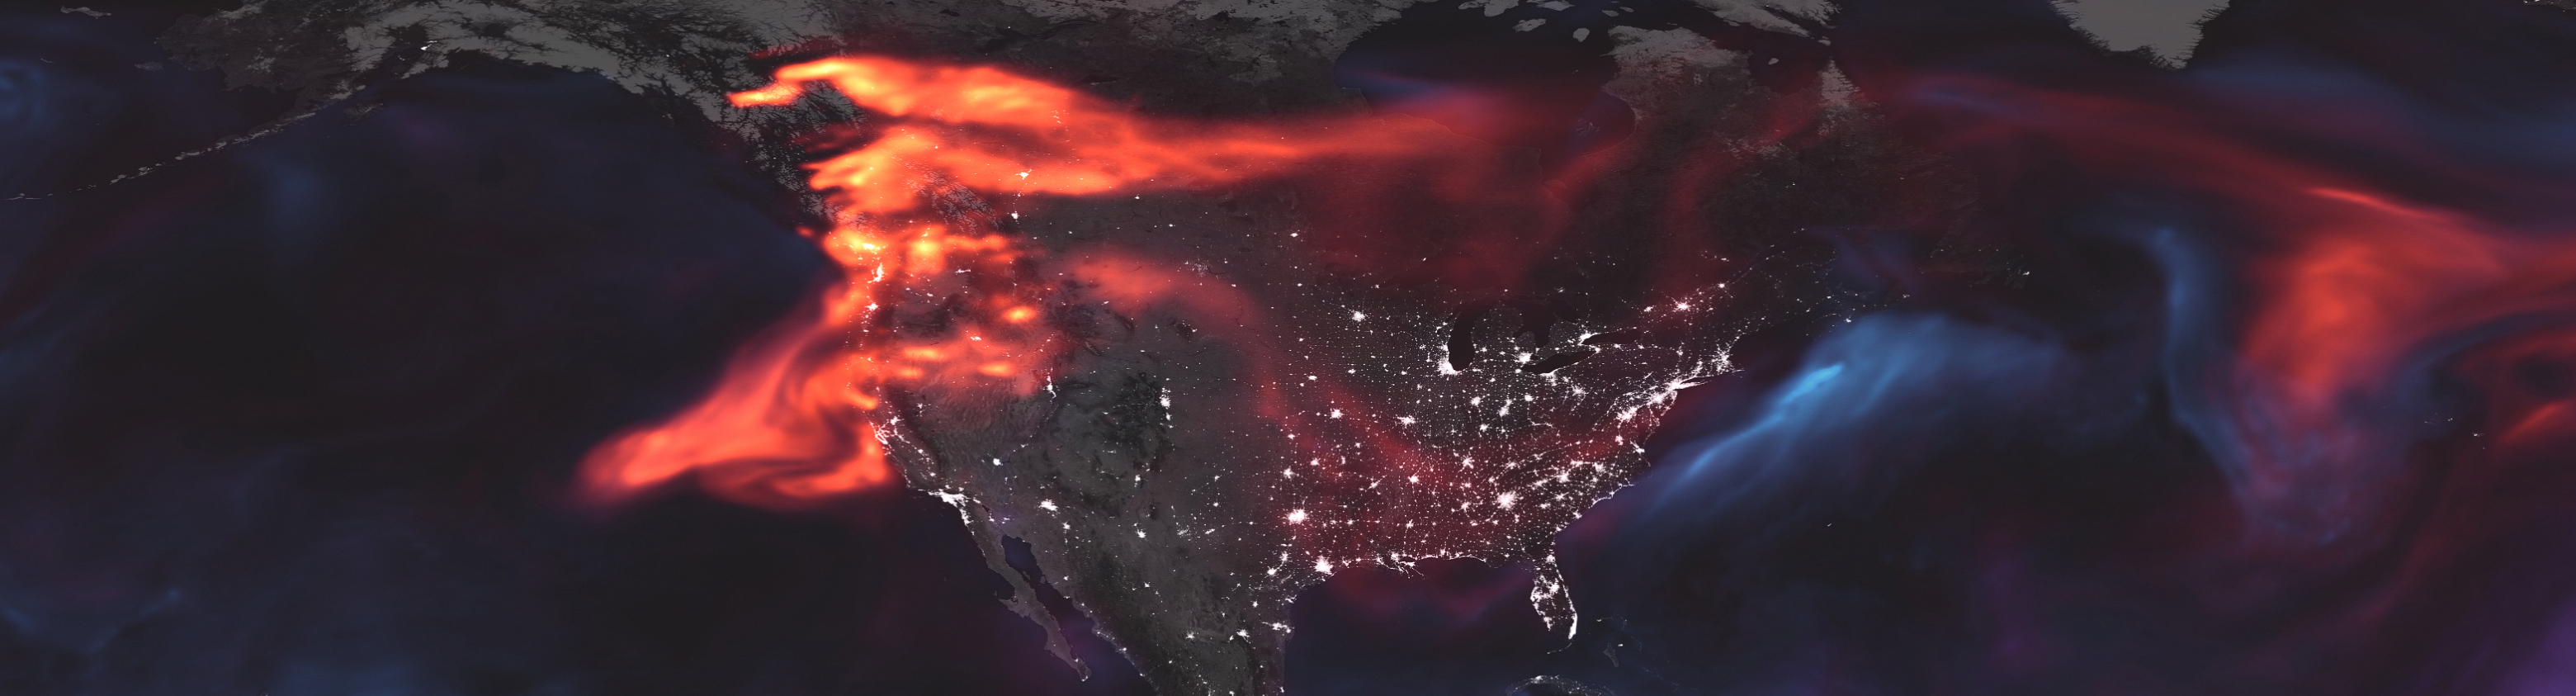
\includegraphics[width=\textwidth]{images/remote_sensing/aerosols_cropped.jpg}
  \caption{A visualization of aerosols over North America on August 23, 2018, using output from NASA's Goddard Earth Observing System Forward Processing model. Black carbon (red) in this image is primarily due to wildfires in the United States and Canada; it can also be emitted by vehicles and factories. Image Credit: NASA/Joshua Stevens/Adam Voiland.}
  \label{teaser}
  \end{figure*}
  
\subsection{Remote Sensing and Analysis}
There has been much research on approaches to analyzing wildfire-related data, though few approaches are practically applicable to real-time scenarios. The authors of~\cite{Coen2013} use remote sensing fire detection data to initialize and evaluate fire growth simulations. In such simulations, uncertainty grows over time; updating the model with the most recent satellite detections helps make sure that the model and the detections are within one another's error bounds. As with modeling fires themselves, modeling the traffic from evacuations is highly dependent on variation and uncertainty in input data. However, approaches such as dynamic traffic assessment (DTA), for planning for evacuations and related traffic, currently assume deterministic inputs, whereas whether an evacuation plan is optimal, or even possible, depends upon the confidence in the inputs~\cite{Yao2009}. (These inputs include properties like specific fire conditions,  and a fire's likelihood of moving in a certain direction.)



%…real-time….
Satellites are increasingly vital to real-time assessment of natural disasters. For one, they help provide relative certainty while ground-based information is often limited, incomplete, or inconsistent, especially during an ongoing disaster~\cite{Voigt2016}. Satellite data are especially promising for filling gaps in current modeling and prediction capabilities. Detections are often provided at more frequent intervals than perimeters, which are reported by humans observing the fire on the ground. 

% * <mvgomov@ucdavis.edu> 2018-07-16T21:09:52.262Z:
% May be worth noting that they provide relative certainty while also being provided at a more regular (& frequent) interval than "on-the-ground" data like perimeters, which are only supplied every ~6-12h (and embargoed by Calfire for some time before they're publicly released as well?) 
% 
% ^.

However, analyzing satellite data involves myriad challenges, including uncertainties from a wide range of sources, and the general difficulty of combining heterogeneous sources~\cite{Luppino2017}. Historical data are widely used to test and hone detection analysis methods. For example, the authors of~\cite{Luppino2017} use clustering analysis to identify changes among heterogeneous satellite images. Interpolated satellite data can be used in the process of making biomass estimates~\cite{Zhang2011}; this links satellite data to what has happened on the ground, to learn how to better interpret satellite data.

%how do things like clouds and smoke affect the analysis we can do of historical fires? how can we use that to help us improve responses to future fires?


Fire radiative power (FRP), estimated from satellite detections, can be used to estimate the total energy released in burning, which in turn can be used to model atmospheric emissions from a fire~\cite{Boschetti2009}. However, this process is highly sensitive to the uncertainties introduced by cloud cover, etc. Estimating the total energy released in a fire (the Fire Radiative Energy, or FRE) is of interest for modeling the atmospheric emissions due to a fire. The authors of~\cite{Boschetti2009} fuse FRP data with burned area data to provide FRE estimates; they attain promising results that are still highly sensitive to the fusion approach and the treatment of uncertainty. FRP can also be used to classify fires into distinct types~\cite{Smith2005}.

Still other applications require more precise information and improved analysis to solve, such as ``spatially and temporally explicit estimates of the quantity of biomass consumed'' in a fire~\cite{Giglio2006}. These estimates may be possible using satellite detections~\cite{Zhang2011}. There is interest in, for example, discovering the correlations between FRP and meteorological information; currently, data available from satellites are generally not detailed enough to be able to make meaningful connections in this area~\cite{Peterson2012b}. Improved tools for visual analysis of historical satellite detections, other related data, and integration with data science techniques can help improve the outlook for advanced wildfire management using satellite detections.

In this study, we present an uncertainty-aware visualization approach for assessing satellite data through several analysis steps: characterizing raw, heterogeneous detections, fusing these detections, and interpolating them. Through a set of case studies, we examine how uncertainty-aware visualization can inform this process, with the potential to improve real-time analysis of satellite fire detections and other sensor data through data science approaches.

%Primarily, our focus is on fusing heterogeneous data to make it accessible for decision-making by emergency management workers. The visualization and analysis in this process is a vital link between gathering raw data and decision-making (either from interpolated detections or from other derived information).

%The ultimate goal is to help emergency managers decide where to allocate resources in a fire, and in general, where the fire will move; this affects structures, roads, pipelines, agriculture, people, and animals.

%what’s the target audience for this? is there a scenario in which the uncertainty part will be useful for users?
%- people honing algorithms (those working on wildfire predictions, or domain experts within emergency management department
%- temp emergency management users (at the endpoint)

%We present the following contributions:
%\begin{itemize}
%\item{An interactive visualization framework for tracking uncertainty through data analysis processes, incl. fusion and interpolation}
%\item{(how much to generalize or narrow this statement?)}
%\item{goal: at each step, we understand the data and uncertainty for proper application of data analysis}
%\item{allow for evolving/varied/domain-specific understanding of what each type of detection means, and therefore how to add it to existing knowledge from other detections}
%\item{``summarize,'' quantitatively, what the satellite data is telling us, in order to put into other fire-related algorithms, etc}
%\end{itemize}

\begin{figure*}[h]
    \begin{subfigure}[t]{0.26\textwidth}
        \centering
        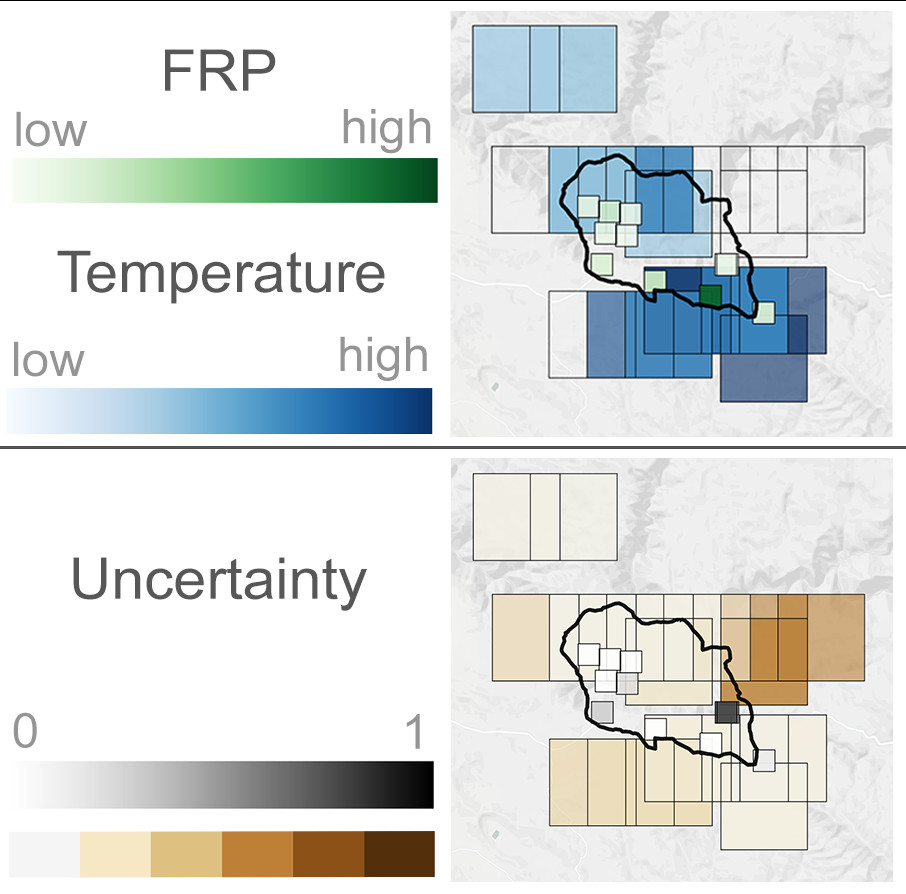
\includegraphics[height=1.6in]{images/remote_sensing/satellite_fusion_diagram_1.jpg}
        \caption{Raw detections.}
        \label{demo_1}
    \end{subfigure}\hfill%
    \begin{subfigure}[t]{0.44\textwidth}
        \centering
        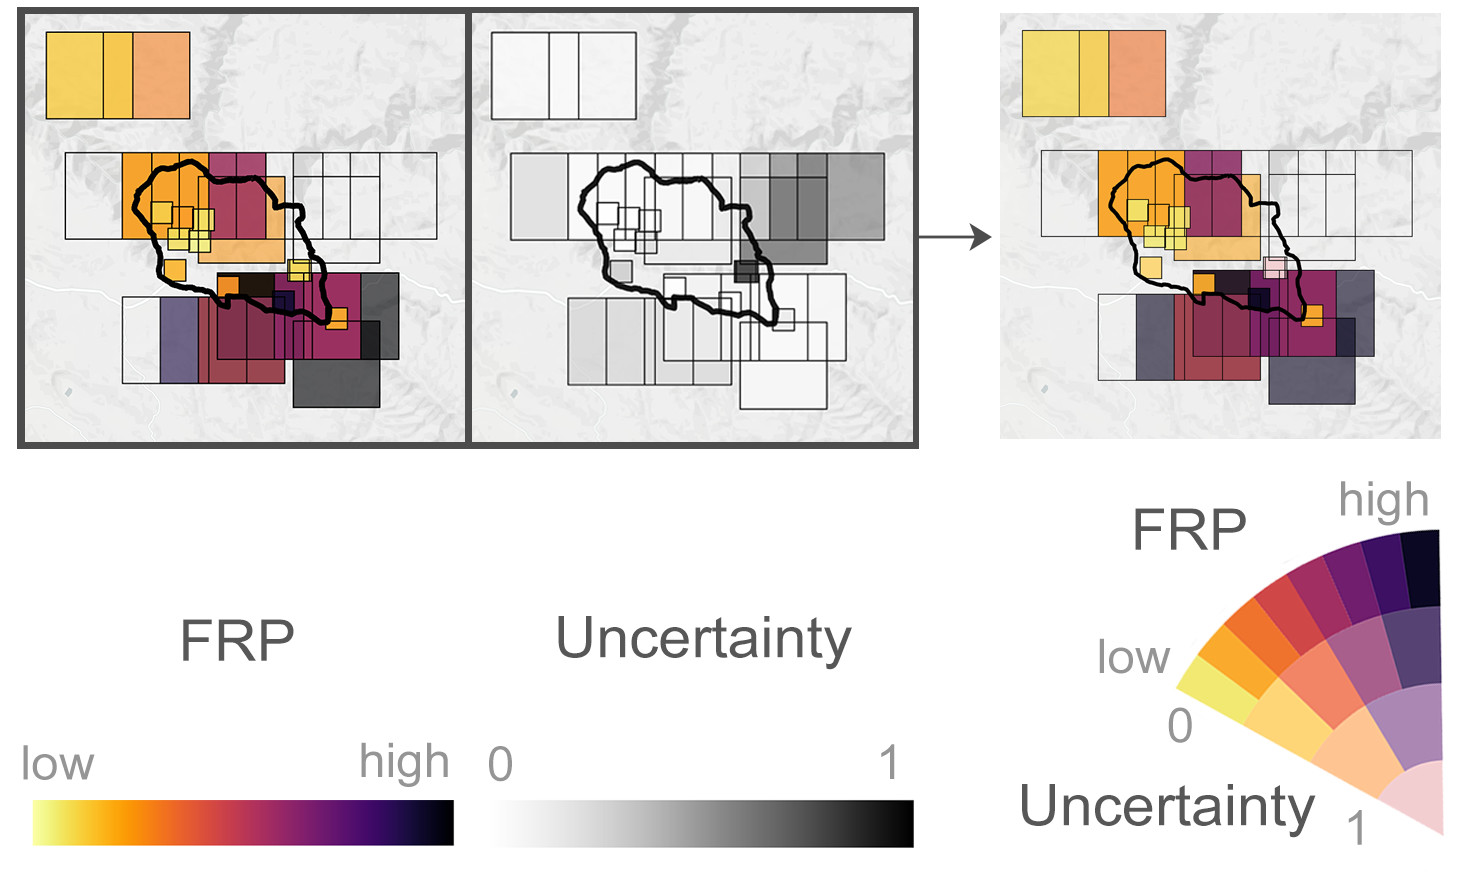
\includegraphics[height=1.6in]{images/remote_sensing/satellite_fusion_diagram_2.jpg}
        \caption{Detections and uncertainties.}
        \label{demo_2}
    \end{subfigure}\hfill%
    \begin{subfigure}[t]{0.26\textwidth}
        \centering
        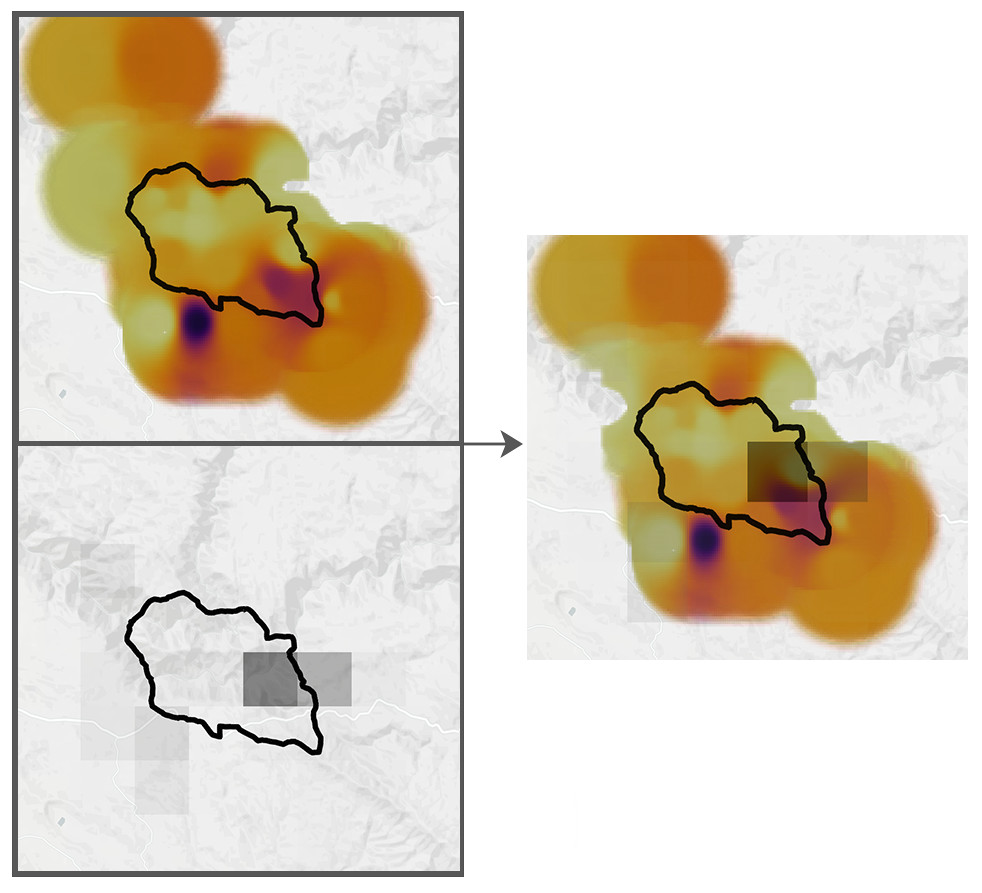
\includegraphics[height=1.5in]{images/remote_sensing/satellite_fusion_diagram_3.jpg}
        \caption{Interpolated detections.}
        \label{demo_3}
    \end{subfigure}
     \caption{Visual encodings to show uncertainty propagating through the data analysis process. \\Step 1 (a): Raw detections from GOES (larger) and MODIS (smaller). Top: FRP and temperature estimates are encoded with different scales; some GOES detections have no temperature estimate. Bottom: uncertainties for each detection, encoded with two different scales, one numerical and one categorical. \\Step 2 (b): Detections and uncertainties are each encoded into a single color scale. Note the high-uncertainty small detection on the right side of the perimeter; this corresponds with a detection showing a low FRP value amid other high detection values. At right, we use a bivariate ``value-suppressing uncertainty palette''~\cite{VSUP} to encode values and uncertainty simultaneously. \\Step 3 (c): Interpolated detections using IDW (top); corresponding uncertainties encoded in a grid (bottom). Combining these images into a single view (right), we see that the uncertainty reflected in the low-FRP detection from Figure~\ref{demo_1} is occluded by the uncertainty grid.}
     \label{summary_figure}
\end{figure*}

\subsection{Data}
We obtained data from two of the most common sources of satellite data for wildfire analysis: NASA's Moderate Resolution Imaging Spectroradiometer (MODIS) and NOAA's Geostationary Satellite Server (GOES). MODIS instruments fly on two ships, Terra and Aqua, each with a different orbit around Earth; we use detections from both. Combining Aqua and Terra data can help eliminate non-detections and decrease the uncertainty in detection rates~\cite{Hawbaker2008}. Additionally, we use detections from two GOES satellites, GOES-13 and GOES-15.

Recently, NASA and USGS have planned to combine GOES and MODIS detections, and others, in real time, to improve the tracking and documentation of fires; many historical fires are missing from state and federal records~\cite{Howard2014}. Therefore, we hope that an exploration of how to analyze these highly heterogeneous data together will be more broadly applicable to other data fusion applications.

%These instruments each have multiple sensors, and report results with different spatial resolutions, at different frequencies, with different measurements and uncertainties. 

%FRP, detections, resolution

%\item{talk about the wide range of uncertainties in the data}
%\item{for example, what does information about what a satellite footprint actually tell us vs. what we need to know? — how likely is the actual detection to be in any part of the footprint? what can we deduce outside the footprint?}


%~\cite{Giglio2006} MODIS can be used to estimate burned area after a fire,,,
%talk about measurements and uncertainties
The GOES detections we obtained have a resolution of 4km, while the MODIS detections have a 1km resolution. GOES provides a temperature estimate if possible, as well as an uncertainty class, such as ``high confidence fire pixel'' or ``saturated fire pixel'' (for more detail, see~\cite{nesdis2010goes}).
MODIS estimates FRP using the temperature, as in~\cite{Freeborn2014}. This calculation introduces uncertainty into the reported value of FRP, especially due to variation of the actual detection location within a satellite pixel.

These detections and estimated temperature and FRP values include uncertainty primarily resulting from cloud cover, smoke cover, and saturation.
There are uncertainties in MODIS detection rates, which makes it hard to accurately interpret statistics derived from detections~\cite{Hawbaker2008}.

FRP is a good characterization of fire intensity~\cite{Peterson2012b}. However, FRP alone is simplistic; for example, an FRP value could be equal for two pixels in different scenarios, such as a large fire with low intensity or a small fire burning with high intensity~\cite{Peterson2012a}. To supplement this information, some high-confidence detections also contain sub-pixel estimates for temperature; we ignore these in this study.

In this study, we consider historical data, but with an aim toward data analysis that could be performed in real time. Additionally, historical study is important on its own. For example, to study and improve decision-making, emergency management workers use historical weather data in simulated scenarios because of the difficulty in simulating weather~\cite{Baumgart2006}. Similarly, modeling fires and weather's effect on fires is difficult, so studying historical fire data (especially in conjunction with historical weather data) is important.

\begin{figure}[t]
    \begin{subfigure}{0.48\textwidth}
        \centering
        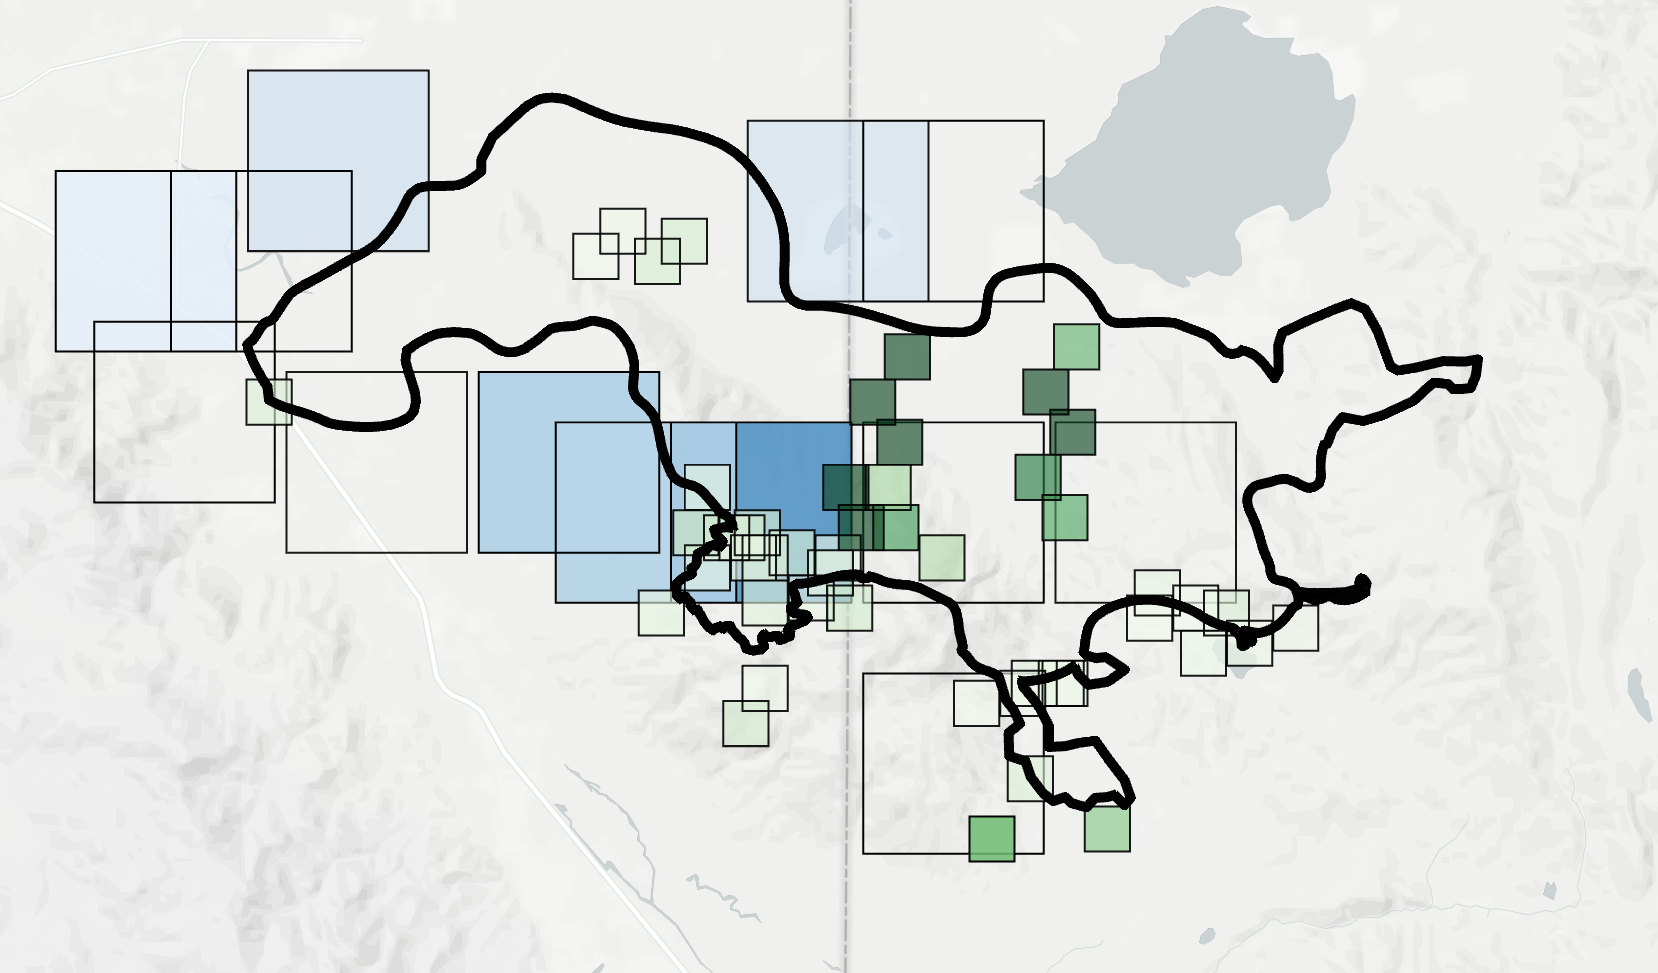
\includegraphics[width=\textwidth]{images/remote_sensing/step_1_example.png}
        \caption{Detections from GOES (temperature mapped to blue) and MODIS (FRP mapped to green) for one 12-hour span. The corresponding perimeter is overlaid.}
        \label{raw_detections}
    \end{subfigure}
    \begin{subfigure}{0.48\textwidth}
        \centering
        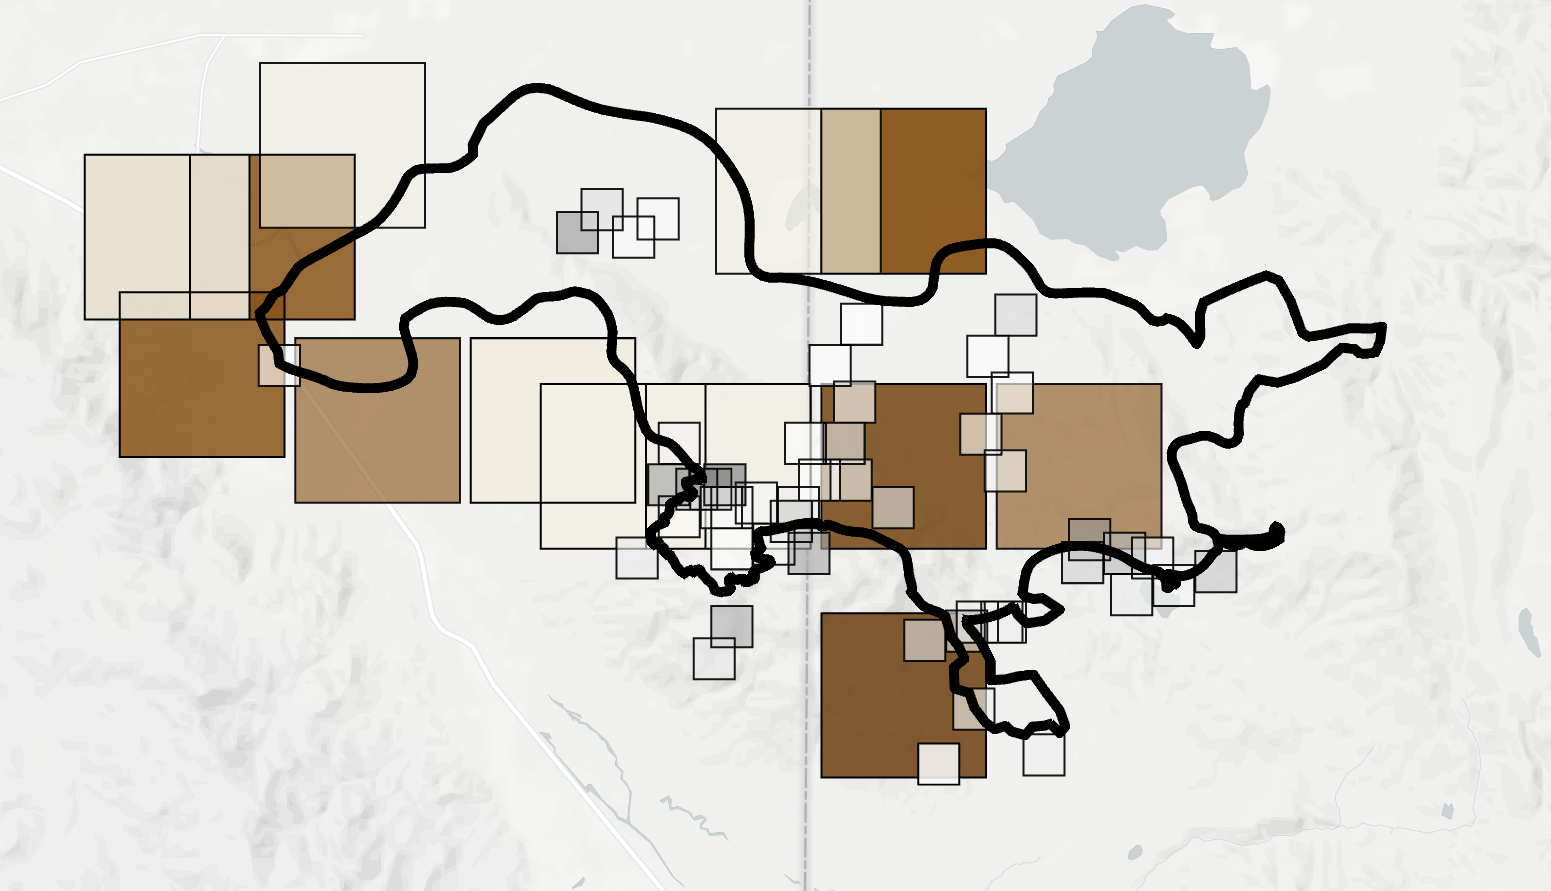
\includegraphics[width=\textwidth]{images/remote_sensing/step_1_uncert.png}
        \caption{Uncertainties from GOES (brown) and MODIS (gray) detections corresponding to Figure~\ref{raw_detections}. Note that GOES footprints can have a confidence level without a corresponding temperature estimate.}
        \label{raw_uncertainty}
    \end{subfigure}
     \caption{Satellite detections and uncertainties for the Long Valley fire in California and Nevada for the last twelve hours of July 14, 2017. The color mappings used are introduced in Figure~\ref{demo_1}.}
     \label{assess_detections}
\end{figure}

\section{Methods}
\label{methods_section}
The primary steps in our analysis are:
\begin{enumerate}
\item{Assess raw (heterogeneous) data}
\item{Fuse data}
\item{Interpolate and analyze data}
\end{enumerate}

\noindent In each step, uncertainty is involved, growing with each transformation. According to~\cite{Pogson2015}, ``the effects of combining aggregated spatial data are found to obey standard properties of error propagation,'' including for resolution-related uncertainty. We employ standard error propagation as appropriate in our calculations. These steps are shown in Figure~\ref{summary_figure}. Before describing our visualization approach, we outline each step in more detail.

\subsection{Assessing Detections}
In this stage, we note that some of the GOES detections have no temperature estimates, but they still have uncertainty values (see Figure~\ref{assess_detections}). We can use this information as desired in the next steps. We can also note areas where detections from different satellites seem to show quite disparate information, and determine whether reported uncertainty explains the discrepancies.  

\subsection{Fusing Data}
Merging multiresolution, multiple-sensor data has several possible approaches, including principal component analysis and high-pass filtering~\cite{Chavez1990}. In our case, there is generally only one value per detection, as opposed to image data, so we use simpler approaches.

First, we would like to merge temperature estimates and fire radiative power (FRP) estimates into a single numerical scale. Temperature and FRP are theoretically related by the Stefan-Boltzmann relationship~\cite{Peterson2012a}:
\begin{equation}
FRP = \sigma(T^4 - T_b^4)A_f
\label{frp_eqn}
\end{equation}
where $\sigma$ is the Stefan-Boltzmann constant, $T$ is the detected temperature, $T_b$ is the background temperature, and $A_f$ is the detected area. In practice, calculating FRP from temperature is complex due to subtleties in determining the background temperature and detected area~\cite{Xu2010}. To measure FRP for individual pixels retrieved by MODIS, a best-fit equation is employed~\cite{Peterson2012a}. For our proof-of-concept, we provided a rough estimate for the conversion between temperature and FRP for GOES detections. Equation~\ref{frp_eqn} could include propagation of uncertainty from the temperature values, but because this is a rough estimate, we do not think it would be meaningful to calculate uncertainty this way at this stage. Figure~\ref{fuse_detections} shows a fused result which we can use to check that the temperature scaling makes sense.

At this stage, we also combine the reported detection uncertainties into a single numerical scale. (We do not yet take uncertainty from multiple resolutions into account.) Detections from MODIS rank uncertainties on a 0-100 scale, while GOES provides categorical designations. To convert between the two, we assign a numerical value to each category (for example, ``medium possibility fire pixel'' = 70, ``high possibility fire pixel'' = 90, ``partially cloudy/smoke fire pixel'' = 30). We can use a fused view to check that these uncertainties are somewhat consistent with one another. Most will be particular to their satellites, but external uncertainties such as cloud or smoke cover should have a similar effect on all detections.

\begin{figure}[h]
     \centering
    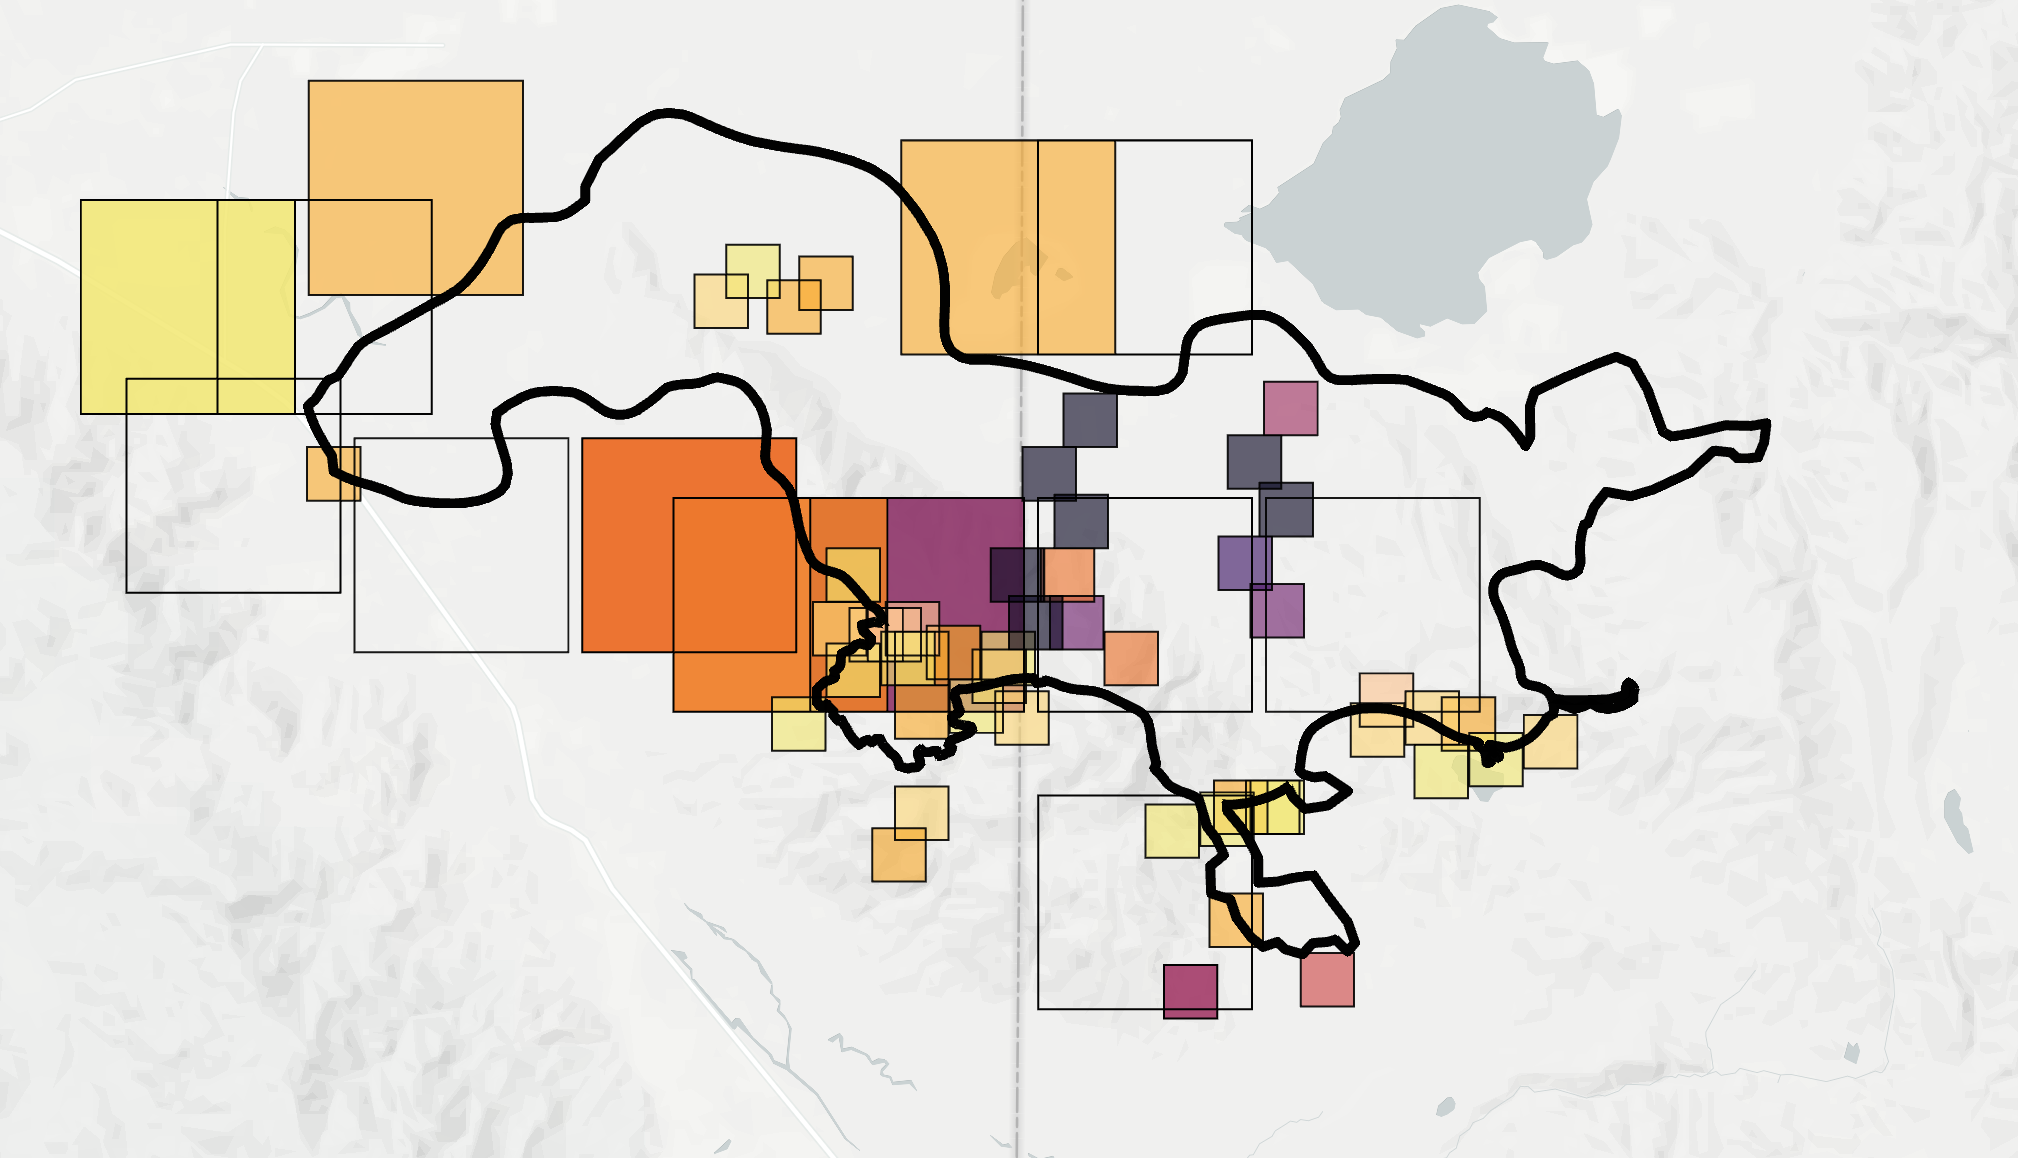
\includegraphics[width=\textwidth]{images/remote_sensing/step_2_example.png}
     \caption{Fused satellite detections and uncertainties for the Long Valley fire, corresponding to data in Figure~\ref{assess_detections}. The VSUP~\cite{VSUP} color mapping used is shown in Figure~\ref{demo_2}.}
     \label{fuse_detections}
\end{figure}

If we combine uncertainty and value (see Section~\ref{visualization}), we must decide what to do with footprints that have no corresponding temperature. Perhaps they can increase the confidence of any other nearby detections if their confidence is relatively high. However, Figure~\ref{raw_uncertainty} shows that the low-confidence GOES detections correspond to those without a temperature estimate, so ignoring these data is also a viable option.

\subsection{Characterization and Analysis}
%The ambiguity introduced by the steps above introduces ambiguity into interpolated outcome.
%how does IDW treat uncertainty ``the right way'' ?
Next, we use data analysis to characterize the satellite detections over a time window. 
\subsubsection{Inverse Distance Weighting}
One approach is to use interpolation techniques to estimate values for points over a smoothed region. Interpolation has been successfully used to supplement incomplete fire information with satellite detection data, such as mapping the day-to-day progression of burning~\cite{Parks2014}. Here, interpolating the timing of satellite detections can make up for the fact that fire perimeters are often incomplete or unavailable. The author of the day-of-burning study compared ten interpolation techniques and found that variations of Weighting by Mean and Distance (WMD) and Inverse Distance Weighting (IDW) provided the best results; however, uncertainty was not taken into account, and no confidence levels were assigned to the predicted values.

In IDW, values are calculated using:

\begin{equation}
V(x) = \frac{\sum_{i=1}^{n}w_i(x)v(x)}{\sum_{i=1}^{n}w_i(x)}
\end{equation}

where the weight is based on the inverse of the distance to some power, $p$:
\begin{equation}
w_i(x) = \frac{1}{\mathrm{dist}(x, x_i)^p}
\end{equation}

IDW can weight either the $n$ nearest neighbors or those within a radius $r$. The latter gives us smoother results. It also makes more sense for this application: our intuition says that detections probably have meaning within some consistent radius, maybe related to their spatial resolution.

Using standard error propagation, we calculate how uncertainty in each detection contributes to uncertainty in the interpolated value:

\begin{equation}
    \sigma_v = \frac{\sqrt{\sum_{i=1}^{n}(w_i
    \sigma_{v_i})^2}}{\sum_{i=1}^{n}w_i(x)}
    \label{idw_uncert}
\end{equation}

To use the result in Equation~\ref{idw_uncert}, we need to know the standard deviation of each temperature or FRP measurement, $\sigma_{v_i}$, but instead, we only have the reported confidence levels or categories, which do not have a clear association with standard deviation. One approach is to supply an estimate of the relative standard deviation, $\sigma_{v_i}/v_i$, for each confidence level. In this application, we are concerned with relative confidence in the measurements, rather than a precise  range of possible values for each measurement, so we propose that this approximation is sufficient for understanding the propagated effect of uncertainty in the measurements.

We could also include the propagated effect of errors in the distances used, as in~\cite{doi:10.1080/10106040801966704}. This would significantly complicate the error calculation. Additionally, there is not a clear way for us to measure the error in the distance between each detection and the sample position. One interpretation could be to assign more uncertainty to lower-resolution satellite detection footprints, indicating that these data provide less precise information about position than do high-resolution footprints. In this study, we choose to assume no error in the sample distances, using only the centroid positions provided for input into the IDW algorithm.

%Kriging is another possible approach to interpolating the detections over an area.

%want to keep original data available (i.e. frp for hovered-over points)
\subsubsection{Kernel Density Estimation}
For our second approach to characterizing satellite detections, we use kernel density estimation (KDE). KDE estimates the probability density function, $f(x)$, of a variable (in this case, FRP):

\begin{equation}
f(x) = \frac{1}{nh}\sum_{i=1}^{n}K(\frac{x-x_i}{h})
\end{equation}

where $K$ is the kernel, and $h$ is the \textit{bandwidth}, which determines how wide a radius
to smooth values over. In this study, we use a Gaussian kernel.

%which kernel do we use?
%how can/does KDE take uncertainty into account?

With this approach, we hope to identify, roughly, the likeliest new and ongoing fire activity around the perimeter. KDE does not put out an uncertainty value; instead, the uncertainty is encoded within the result itself. That is, detections with higher uncertainty are assigned lower weights. Therefore, we can inspect uncertainty through the rest of the pipeline, leading up to performing KDE, to assess whether it looks like uncertainty information has been properly incorporated.
%briefly weighting

%how does it take reference and target time into account?

%can i weight the more recent detections more heavily?

\subsection{Visualization Approach}
\label{visualization}

As much as possible, our encodings should be ``informationally equivalent'' throughout the data analysis steps, which is difficult because uncertainty introduces a lot of complexity and clutter to maps~\cite{Kinkeldey2014b}. Ideally, adding more information to an image should not look like ``more fire'' is being added, just that we are more certain about the information that is there. Above all, our encodings should be intuitive to someone without much specialized knowledge. While emergency managers such as our collaborator have extensive knowledge of fire-related data, during an ongoing event, workers who do not have specific emergency management expertise may be brought in; any tool supporting decision-making with visual analysis should be easily accessible to them. The visualization approaches we use are summarized in Figure~\ref{summary_figure}.

In a survey of geospatial-uncertainty-related user studies~\cite{Kinkeldey2014b}, the authors identify three main dichotomies: intrinsic/extrinsic; coincident/adjacent; static/dynamic. We explore these axes to apply the appropriate uncertainty visualization mode for each step in our data analysis.
 
No significant distinctions are found between coincident and adjacent approaches~\cite{Kinkeldey2014b}. Here, we aim for coincident when possible (i.e., when the information is reduced enough for meaningful coincident encodings); it seems easier on the mental map. Most approaches surveyed used static images rather than dynamic, animated approaches. For simplicity, we focus on static images representing a chosen time window.

\begin{center}
    \begin{tabu} {p{2.2cm}|p{10cm}X[l]}
          Coincident & Use if possible: easier for the mental map\\
          \midrule
        Adjacent & Use if there is too much information to meaningfully include with data 
    \end{tabu}
\end{center}

For intrinsic uncertainty depiction, the authors find that from the studies surveyed, hue, value, and transparency are best for conveying uncertainty (with darker representing higher uncertainty being most effective)~\cite{Kinkeldey2014b}. The Value-Suppressing Uncertainty Palette (VSUP)~\cite{VSUP} creates a bivariate map for encoding value-uncertainty combinations (see Figure~\ref{summary_figure}). One goal of this approach is to improve decision-making by making it harder for the user to distinguish between uncertain states, and easier to make precise distinctions when uncertainty is low. 

\begin{figure*}[h]
    \begin{subfigure}[t]{0.5\textwidth}
        \centering
        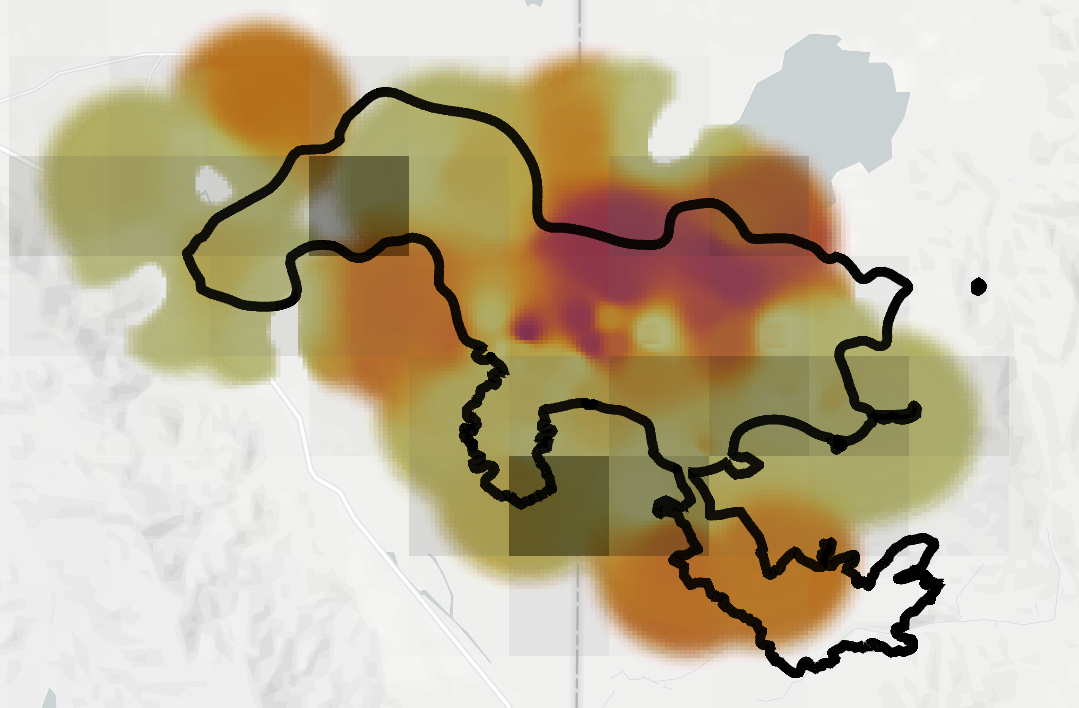
\includegraphics[height=2in]{images/remote_sensing/idw_casestudy_p4_r3_5.png}
        \caption{IDW results with $p=4$, $r=3.5\mathrm{km}$. The next available perimeter is overlaid.}
        \label{idw_result_1}
    \end{subfigure}
    \begin{subfigure}[t]{0.48\textwidth}
        \centering
        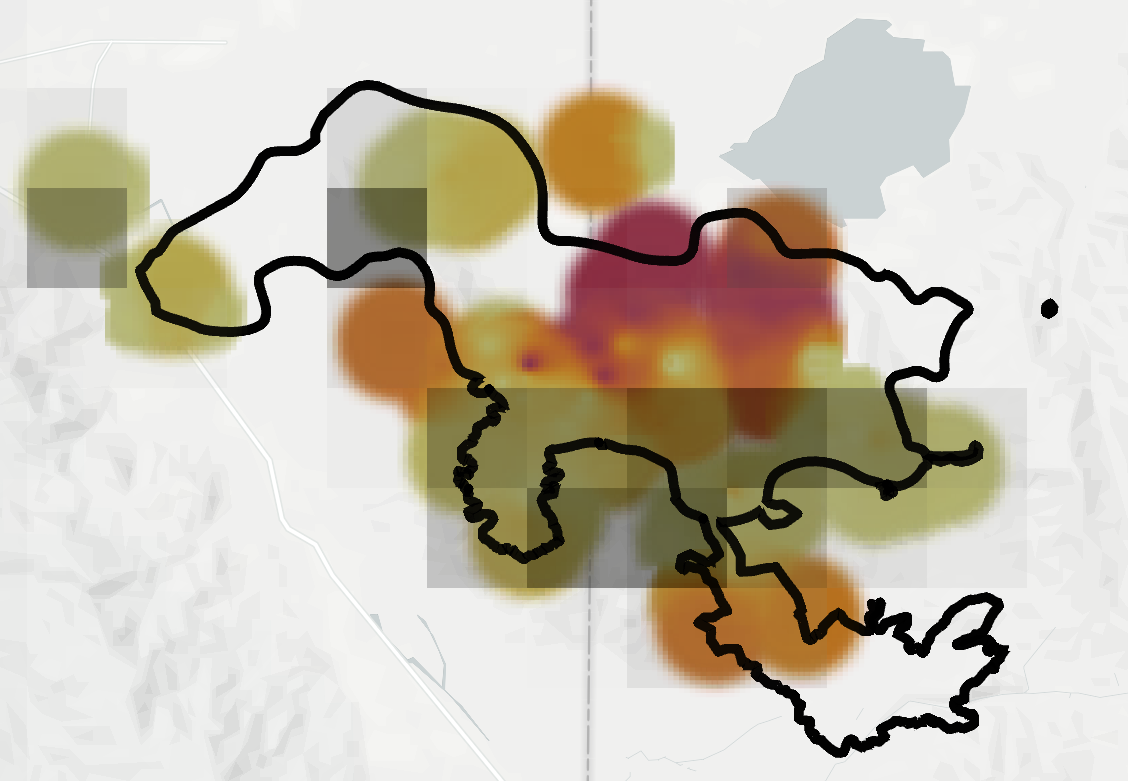
\includegraphics[height=2in]{images/remote_sensing/idw_casestudy_p2_r1_8.png}
        \caption{IDW results with $p=2$, $r=1.8\mathrm{km}$. The next available perimeter is overlaid.}
        \label{idw_result_2}
    \end{subfigure}
     \caption{Using Inverse Distance Weighting to characterize fire behavior. The color map (non-VSUP version) is introduced in Figure~\ref{demo_2}, with yellow corresponding to lower activity and purple corresponding to higher activity.}
     \label{idw_ref}
\end{figure*}

%``there’s a limited budget for perceptual discriminability''

%quantization error vs. perceptual error
Extrinsic techniques are used in fewer of the studies surveyed in~\cite{Kinkeldey2014b}, but are recommended in cases where color is already used to depict values, such as in map-based visualizations~\cite{Kinkeldey2014a}. The authors of~\cite{Kinkeldey2014a} implement grid-based uncertainty for maps using lines depicted with varying amounts of visual noise. They find that how users perceive the uncertainty depends strongly on the number of levels. This can be ameliorated somewhat by maximizing relative differences between encodings, but complex ``mixed'' uncertainty information, as in our application, makes this hard. Grid-based methods can also vary the size of the grid to indicate uncertainty level, such as using a tessellated quadtree in~\cite{Kardos2007}.

\begin{center}
    \begin{tabu} {p{2cm}|p{8cm}X[l]}
        Intrinsic & Use when uncertainty is a property of each item \\
        \midrule
        Extrinsic & Use when uncertainty is more accurately defined over a region  \\
    \end{tabu}
\end{center}

We use intrinsic methods to depict satellite detections, but switch to a grid-based visualization once the data are interpolated, because this step introduces more complex color encoding. Because the interpolated images are complex, we aim for a simpler grid-based uncertainty visualization than the examples above. Our implementation includes a grid with cells of fixed pixel size, showing more detail as a user zooms in. Each cell is colored with a grayscale value corresponding to the aggregated relative interpolated uncertainty in that area (see Figure~\ref{demo_3}).

%discuss:
%- smoke analogy (grid-based method!) doesn’t make sense for the individual detections, since superimposing a grid would be arbitrary.
%- another principle we use: one scale (color) per unique data scale; this goes for values and their uncertainties.
%- what does each view/encoding show us?
%talk about the use of opacity: here, to (kind of) indicate uncertainty in the %``where''

%**NOTE that, when we fuse data and some footprints have a confidence value but no measurement value, it’s hard to depict faithfully in the VSUP

%used a perceptually uniform color scale, which seems to make the best VSUPs
%additionally, we should be visualizing `what’ and `where’ for our selected time window; in this step, `where’ gets a lot more uncertain.)

\subsection{Validation}
Quantifying success for an IDW or KDE result is difficult for several reasons. One simple approach is to compare interpolated fire activity with changes in perimeters. However, we are not making predictions, only summarizing the detected activity. Therefore, there is no ``ground truth'' to compare to. Whether the important features are captured may require expert users to determine. Additionally, perimeters are often made available significantly later (12-14 hours) than the time they reflect, so comparison with perimeters will be especially limited in real-time analysis.

However, there are varying degrees of success, and the summary does not need to be perfect to be helpful. According to our primary emergency management collaborator, knowing the direction of the fire and which general areas to send supplies to are some of the most important factors for rapid decision-making. We can rely on visual analysis to see whether our results accurately reflect
the relative levels of activity within a fire. For visual comparison, we obtain historical fire perimeters from the Geospatial Multi-Agency Coordination (GeoMAC) (www.geomac.gov).

For more thorough validation, we plan to survey emergency management practitioners in a future study, assessing how our visualization approach would impact their decision-making in historical wildfire scenarios. 

\section{Case Studies}
The case studies focus on the Long Valley Fire in California and Nevada during July 2017.

%\subsection{Fusion} 
%do uncertainties have good agreement? (i.e. clouds/smoke have clear patterns?)
%External sources of uncertainty, such as clouds or smoke obscuring satellite detections, should consistently affect observations from both MODIS and GOES satellites. Where images of the fused data agree on areas of high uncertainty, clouds or smoke may be the cause. Disagreements in the fused image, however, likely originate from other causes (see Figure ??). Adjusting the uncertainty scalings, and inspecting the resulting fused visualization, can inform how to interpret the satellite detections. [for example, ... ]

\subsection{Interpolation}
\label{interpolation}

Uncertainty-aware visualization can help improve the algorithms we use to interpolate the detections. One set of detections and their uncertainties are shown in Figure~\ref{fuse_detections}. There are three areas of activity in the lower right part of the current perimeter. The middle cluster contains detections from two different satellites, though the lower-resolution detection is also highly uncertain. The middle and right clusters each contain 6-7 higher-resolution detections with roughly similar, low uncertainty distributions. The left-most cluster contains the most detections from both satellites, with fewer low-confidence detections. Additionally, two medium-high confidence detections from one satellite lie outside the current perimeter near the cluster. 

An IDW interpolation of these detections, with the next available fire perimeter, is shown in Figure~\ref{idw_result_1}.  Of the three clusters identified near the perimeter in the first timestep, the left two turned out to indicate areas where the fire was expanding. Analyzing this outcome can help us optimize an interpolation of these data to be as informative as possible.

\begin{figure}[h!]
    \begin{subfigure}{0.48\textwidth}
    \centering
    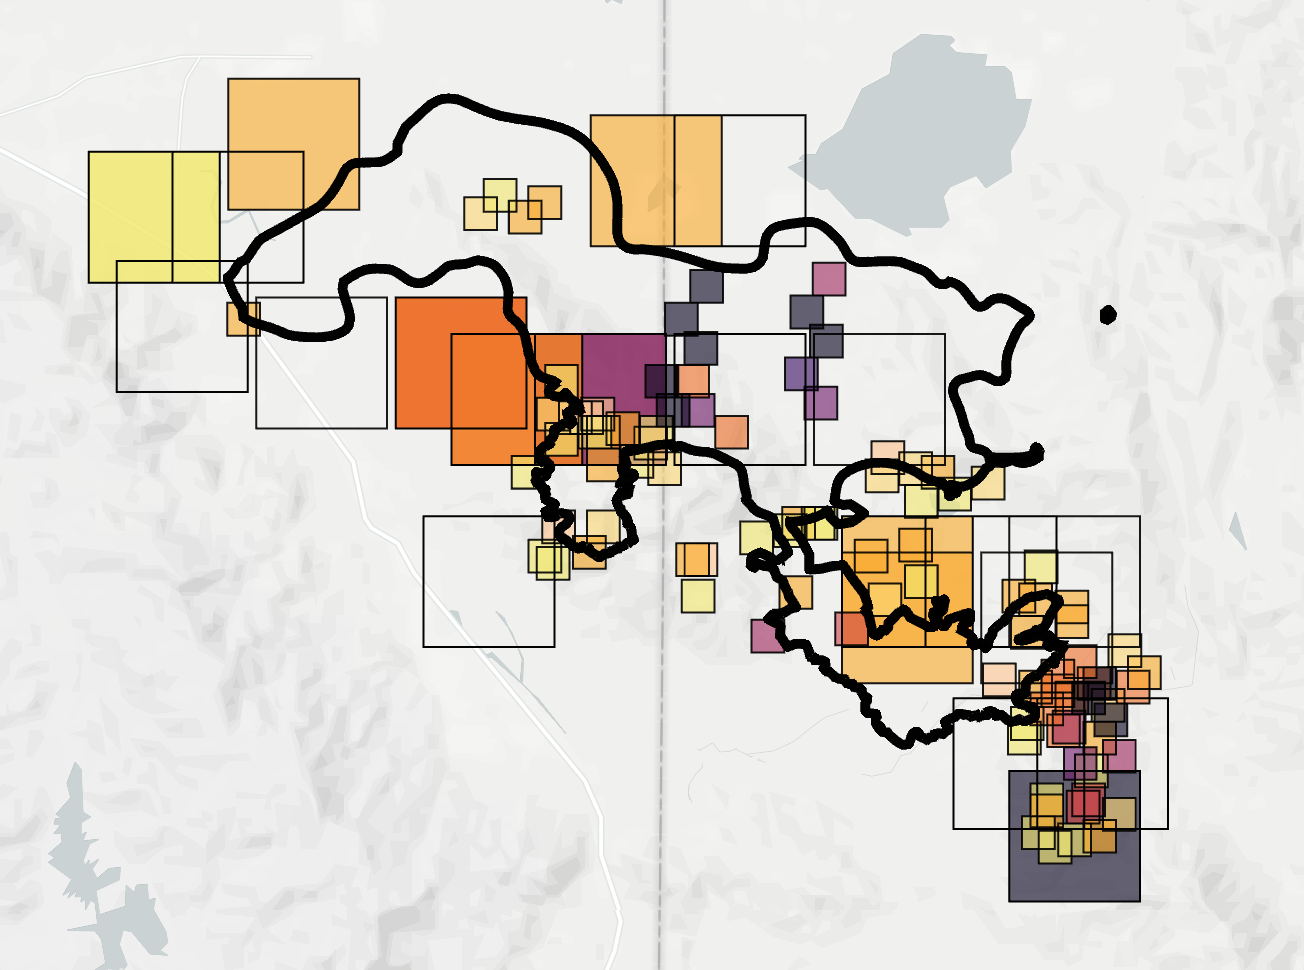
\includegraphics[width=\textwidth]{images/remote_sensing/kde_reference.png}
    \caption{Detections (with uncertainty encoded using a VSUP~\cite{VSUP}) for a later 12-hour span of the Long Valley fire.}
    \label{kde_ref}
    \end{subfigure}
    
    \begin{subfigure}[c]{0.48\textwidth}
    \centering
    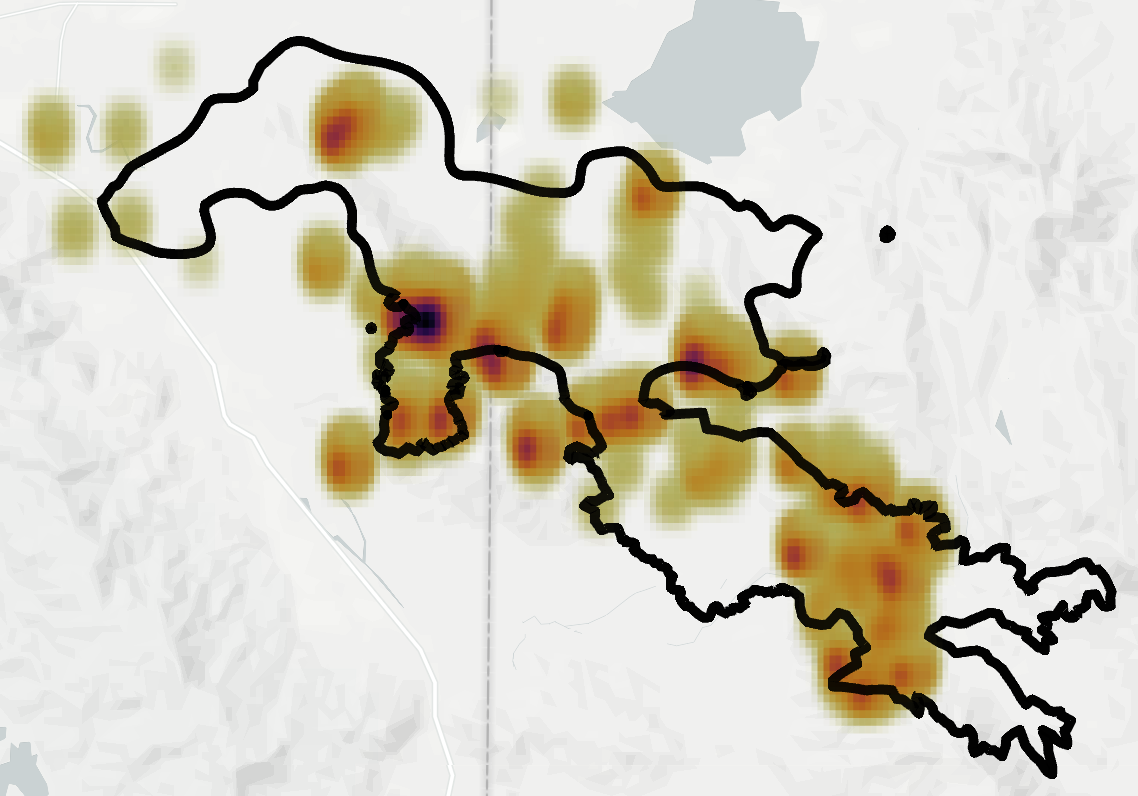
\includegraphics[width=\textwidth]{images/remote_sensing/bandwidth_a_next.png}
    \caption{KDE result showing the areas of heaviest activity. The next available perimeter is overlaid, showing the fire extending southeast.}
    \label{kde_a}
    \end{subfigure}
    
    \begin{subfigure}[c]{0.48\textwidth}
    \centering
    \includegraphics[width=\textwidth]{images/remote_sensing/adjusted_next.png}
    \caption{Adjusted KDE result to reflect ``smoothing'' the influence of the lower-resolution detections. This result more strongly predicts the fire's spread south and east.}
    \label{kde_b}
    \end{subfigure}
    \caption{Using Kernel Density Estimation to characterize fire behavior.}
\end{figure}

First, both of the leftmost clusters are somewhat loosely distributed, whereas the rightmost one is tightly centered on the existing perimeter. This tells us that perhaps more uncertain detections should ``spread'' their values over a larger radius than more certain detections do, but with less confidence. Also, maybe having one detection slightly beyond the border of the rest of the cluster is indicative of more movement. Because the detections in the right-most cluster were entirely in a tight group with relatively high confidence, the interpolated result should show a lower probability that those detections indicate spreading.

An adjusted interpolation result is shown in Figure~\ref{idw_result_2}. This result puts less emphasis on potential spread to the east, and indicates more variability in the detections that indicate expansion to the south. As opposed to the first result in Figure~\ref{idw_result_1}, analysts looking at this interpolation might not focus as many resources to the east side of the fire, and might focus more on the volatility in the southern direction.

\subsection{Density and Multiple Resolutions}
\label{kde}
We explore the use of Kernel Density Estimation (KDE) to find the areas of highest activity. For reference, the detections we analyze here appear in Figure~\ref{kde_ref}. The KDE calculation considers uncertainty by adjusting detection weights according to relative confidence levels. The result of one KDE implementation is shown in Figure~\ref{kde_a}. For example, the two faint orange, large footprints at the top of Figure~\ref{kde_ref} indicate low confidence, and accordingly, they are encoded as relatively insignificant in the KDE result. 

However, this approach only considers detection uncertainty, not the uncertainty that arises from combining detections with multiple resolutions. One way to address this in the KDE algorithm might be to scale the GOES (i.e., larger footprint) confidence values slightly downward, indicating that for these detections, we are less sure about the exact positions of their influence. The result of this uncertainty scaling adjustment is shown in Figure~\ref{kde_b}. The difference is subtle, but the adjusted scaling creates stronger emphasis on the southeast portion, where the fire growth is most extreme. (Another way to incorporate uncertainty from multiple resolutions, not shown here, might be to increase the bandwidth of the kernels corresponding to lower-resolution footprints.)

To continue fine-tuning the uncertainty encodings, one could use the separate and fused uncertainty views (Figures~\ref{demo_1},~\ref{demo_2}) to check how much the scaling is warping the underlying data. 


\section{Conclusions}
In order to move toward the goal of vastly improving satellite-assisted emergency management, we need to advance the capabilities of data mining and big data analysis platforms for geographical data~\cite{Voigt2016}. Applying data science techniques to sensor data, though, is fraught with difficulties, including (but not limited to) uncertainty. Visual analytics, using an approach like ours, could provide a helpful tool as data scientists and emergency managers work together to improve analytic and predictive capabilities from satellite (and other) data. A tool such as ours could provide a shared communication method that can be useful for people with both types of expertise.

This visualization approach was motivated by the early stages of our collaboration with local emergency managers. To create usable decision support tools for emergency managers, we next need to conduct studies of usability and decision-making potential with our approach. Additionally, we can conduct a much wider survey of the possible data analysis approaches for satellite detection data and how visualization can assist in those analyses. Finally, the lessons learned should be applicable to emergency management and disaster preparedness in domains outside of wildfires, such as floods, hurricanes, and earthquakes.

%% if specified like this the section will be committed in review mode
\acknowledgments{
This research is sponsored in part by the U.S. National Science Foundation through grant IIS-1320229  and the U.S. Department of Energy through grant DE-SC-0012610. The authors also thank Dana Carey, the Office of Emergency Services Coordinator for Yolo County, CA.
}
\chapter{Ongoing Work}

\section{Interpretable Clustering with User Feedback}
\subsection{Problem Statement}
\subsection{Defining a Space of Feature Representations}
\subsection{Learning Decision Trees for Interpretable Clusters}

\section{Remote Sensing Visualization with Transparent Belief Updating}

\section{Unified Workflow for Simulation Data}

\section{Unified Workflow for Sensing Data}

\section{Schedule}

\bibliography{ucdavisthesis_example}

% The UMI abstract uses square brackets!
% \UMIabstract[The UMI abstract is submitted online as plain text. It no longer has a word limit or specific formatting. Therefore, the UMIabstract command is now deprecated.]

\end{document} 